%% Copernicus Publications Manuscript Preparation Template for LaTeX Submissions
%% ---------------------------------
%% This template should be used for copernicus.cls
%% The class file and some style files are bundled in the Copernicus Latex Package, which can be downloaded from the different journal web pages.
%% For further assistance, please contact Copernicus Publications at: production@copernicus.org
%% https://publications.copernicus.org/for_authors/manuscript_preparation.html


%% Please use the following documentclass and journal abbreviations for preprints and final revised papers.

%% 2-column papers and preprints
%\documentclass[journal abbreviation, manuscript]{copernicus} % default
%\documentclass[gmd, preprint]{copernicus}
\documentclass[manuscript]{copernicus}


%% Journal abbreviations (please use the same for preprints and final revised papers)


% Advances in Geosciences (adgeo)
% Advances in Radio Science (ars)
% Advances in Science and Research (asr)
% Advances in Statistical Climatology, Meteorology and Oceanography (ascmo)
% Annales Geophysicae (angeo)
% Archives Animal Breeding (aab)
% Atmospheric Chemistry and Physics (acp)
% Atmospheric Measurement Techniques (amt)
% Biogeosciences (bg)
% Climate of the Past (cp)
% DEUQUA Special Publications (deuquasp)
% Drinking Water Engineering and Science (dwes)
% Earth Surface Dynamics (esurf)
% Earth System Dynamics (esd)
% Earth System Science Data (essd)
% E&G Quaternary Science Journal (egqsj)
% EGUsphere (egusphere) | This is only for EGUsphere preprints submitted without relation to an EGU journal.
% European Journal of Mineralogy (ejm)
% Fossil Record (fr)
% Geochronology (gchron)
% Geographica Helvetica (gh)
% Geoscience Communication (gc)
% Geoscientific Instrumentation, Methods and Data Systems (gi)
% Geoscientific Model Development (gmd)
% History of Geo- and Space Sciences (hgss)
% Hydrology and Earth System Sciences (hess)
% Journal of Bone and Joint Infection (jbji)
% Journal of Micropalaeontology (jm)
% Journal of Sensors and Sensor Systems (jsss)
% Magnetic Resonance (mr)
% Mechanical Sciences (ms)
% Natural Hazards and Earth System Sciences (nhess)
% Nonlinear Processes in Geophysics (npg)
% Ocean Science (os)
% Polarforschung - Journal of the German Society for Polar Research (polf)
% Primate Biology (pb)
% Proceedings of the International Association of Hydrological Sciences (piahs)
% Safety of Nuclear Waste Disposal (sand)
% Scientific Drilling (sd)
% SOIL (soil)
% Solid Earth (se)
% The Cryosphere (tc)
% Weather and Climate Dynamics (wcd)
% Web Ecology (we)
% Wind Energy Science (wes)

%% \usepackage commands included in the copernicus.cls:
%\usepackage[german, english]{babel}
\usepackage{tabularx}
\usepackage{tablefootnote}
%\usepackage{datetime2}  % \DMTnow
\usepackage[en-GB]{datetime2} % \usepackage[en-GB,en-US]{datetime2}
\DTMlangsetup[en-GB]{ord=raise,abbr,monthyearsep={,\space}}
% https://www.dickimaw-books.com/faq.php?itemlabel=datetime2adjustregional
%\usepackage{hyperref}
%\usepackage{cancel}
%\usepackage{multirow}
%\usepackage{supertabular}
%\usepackage{algorithmic}
%\usepackage{algorithm}
%\usepackage{amsthm}
%\usepackage{float}
%\usepackage{subfig}
%\usepackage{rotating}
%%\usepackage{xparse} %% required for multicite custom function
\usepackage[inkscapelatex=false]{svg} %% use SVG graphics
% https://forum.manjaro.org/t/getting-usepackage-svglatex-in-texstudio-to-work/140125/7 - texstudio

%% force \autoref capitalization
\def\sectionautorefname{Section}
\def\subsectionautorefname{Section}
\def\subsubsectionautorefname{Section}
\def\subsubsubsectionautorefname{Section}

%% define user commands
\newcommand{\mycomment}[1]{}
% autoref capitalisation
% https://tex.stackexchange.com/questions/34155/autoref-does-not-capitalize-initial-character-in-sentence-when-referencing-labe

% Takes a pair of citations with an optional prefix
% https://tex.stackexchange.com/questions/172699/several-citations-in-the-same-bracket
%\newcommand{\multicite}{ogog}{%
%    \citetext{%
%        \IfValueT{#2}{%
%            \IfValueT{#1}{\citealp[#1;]{#2}}%
%            \IfNoValueT{#1}{\citealp{#2}}%
%        }%
%        \IfValueT{#4}{%
%            ;
%            \IfValueT{#3}{\citealp[#3;]{#4}}%
%            \IfNoValueT{#3}{\citealp{#4}}%
%        }%
%    }
%}

% Define colours to capture author contributions
\def\cred#1{{\color{red}#1}}
\def\cblue#1{{\color{blue}#1}}


\begin{document}

\title{The Coupled Model Intercomparison Project (CMIP): Reviewing project history, evolution, infrastructure, and implementation}
\mycomment{
Veronika E alternate: The Coupled Model Intercomparison Project (CMIP): Reviewing project history, evolution, and infrastructure; it would be nice if the title could somehow include the word ``infrastructure'', as it is a big part of the paper. Maybe replace future with infrastructure? Karl: I like that idea
was: The Coupled Model Intercomparison Project phase 6 (CMIP6): A review of project evolution and future
Pete G alternate: The Coupled Model Intercomparison Project phase 6 (CMIP6) was made possible by an evolution of project implementation
Jiwoo alternate: The Coupled Model Intercomparison Project (CMIP): a review of project history, evolution and future
}

% \Author[affil]{given_name}{surname} % Author {first initial.}{last}
\Author[1]{Paul J.}{Durack} % ORCID 0000-0003-2835-1438
\Author[1]{Karl E.}{Taylor} % 0000-0002-6491-2135
\Author[1]{Peter J.}{Gleckler} % 0000-0003-2816-6224
\Author[2]{Gerald A.}{Meehl} % 0000-0002-8760-9534
\Author[3]{Bryan N.}{Lawrence} % 0000-0001-9262-7860
\Author[1]{Curt}{Covey} % 0000-0002-0016-7199
\Author[4]{Ronald J.}{Stouffer} % 0000-0002-7900-6290
\Author[5,6]{Guillaume}{Levavasseur} % 0000-0002-0801-0890
\Author[5,7]{Atef}{Ben-Nasser} % 0000-0001-6948-8735
\Author[8,a]{Sebastien}{Denvil} % 0000-0002-6715-3533
\Author[9]{Martina}{Stockhause} % 0000-0001-6636-4972
\Author[3,10]{Jonathan M.}{Gregory} % 0000-0003-1296-8644
\Author[11,12]{Martin}{Juckes} % 0000-0003-1770-2132
\Author[13]{Ian T.}{Foster} % 0000-0003-2129-5269
%---
\Author[1]{Sasha K.}{Ames} % 0000-0001-9981-2997
\Author[14]{Fabrizio}{Antonio} % 0000-0002-7693-0111
\Author[1]{David C.}{Bader} % 0000-0003-3210-339X
\Author[15]{John P.}{Dunne} % 0000-0002-8794-0489
\Author[16]{Daniel}{Ellis} % 0000-0001-6733-7028
\Author[17,18]{Veronika}{Eyring} % 0000-0002-6887-4885
\Author[19,b]{Sandro L.}{Fiore} % 0000-0002-8430-6087
\Author[5,7]{Sylvie}{Joussaume} % 0000-0002-1510-3964
\Author[20,12]{Philip}{Kershaw} % 0000-0002-7646-291X
\Author[c]{Jean-Francois}{Lamarque} % 0000-0002-4225-5074
\Author[d]{Michael}{Lautenschlager} % no ORCID
\Author[1]{Jiwoo}{Lee} % 0000-0002-0016-7199
\Author[1]{Chris F.}{Mauzey} % 0000-0003-1156-6774
\Author[10]{Matthew}{Mizielinski} % 0000-0002-3457-4702
\Author[14]{Paola}{Nassisi} % 0000-0003-2857-4391
\Author[14]{Alessandra}{Nuzzo} % 0000-0002-8801-6917
\Author[16]{Eleanor}{O'Rourke} % 0000-0002-0775-0811
\Author[e]{Jeffrey}{Painter} % 0000-0001-7920-4337
\Author[e]{Gerald L.}{Potter} % 0000-0003-0291-7229
\Author[5,6]{Sven}{Rodriguez} % 0009-0000-4283-3228
\Author[f]{Dean N.}{Williams} % no ORCID

%\Author[xx]{and past/present members of the}{WGCM Infrastructure Panel (WIP), CMIP Panel, and Earth System Grid Federation (ESGF)}
%\Author[30\textdagger]{others please}{add yourselves - will alphabetically reorder once final}
% Edits: Jerry, Bryan, Curt, Ron, Guillaume, Atef, Sebastien;
% Feedback: Jeff, Martin, Veronika, Martina, Dave, Gerry, Sandro, Alessandra
% Jerry: tracked changed edits
%\autoref{sec:cmip6InContext,sec:cmip6ProjectDesign}
% Bryan: tracked changed edits
%\autoref{sec:CFConventions,sec:earthSystemGridFederation,sec:ModelDocumentation}
% Curt: Written edits
% Ron: email edits
% Guillaume, Atef, Sebastien: https://docs.google.com/document/d/1bb_3GdAXgiPrcAIUZhydNbAXfcv9zkwuAFuVSLWkQ8E/edit
%\autoref{sec:CMIPDataReplication,sec:CMIPErrata}
% Martina: https://docs.google.com/document/d/1aQbZj6xQYr-5_Ub9tw9hucm6WzcPIImYMShONPYrpyo/edit
%\autoref{sec:IPCC-DDC,sec:DataCitation}
% Jonathan:
%\autoref{sec:CFConventions}
% Martin:
%\autoref{sec:CMIP6DR}

% \affil % Affiliations
\affil[1]{Program for Climate Model Diagnosis \& Intercomparison (PCMDI), Lawrence Livermore National Laboratory (LLNL), Livermore, California, USA}
\affil[2]{National Center for Atmospheric Research (NCAR), Boulder, Colorado, USA}
\affil[3]{NCAS, Department of Meteorology, University of Reading, Reading, UK}
\affil[4]{The University of Arizona (UA), Tucson, Arizona, USA}
\affil[5]{Institut Pierre Simon Laplace (IPSL), Paris, France}
\affil[6]{Sorbonne University (SU), Paris, France}
\affil[7]{Centre National de Recherche Scientifique (CNRS), Paris, France}
\affil[8]{European Centre for Medium-Range Weather Forecasts (ECMWF), Reading, UK}
\affil[9]{German Climate Computing Center (DKRZ), Hamburg, Germany}
\affil[10]{Met Office (MOHC), Exeter, UK}
\affil[11]{Kellogg College, University of Oxford, Oxford, UK}
\affil[12]{UK Research and Innovation (UKRI) Science \& Technology Facilities Council (STFC), Oxfordshire, UK}
\affil[13]{Argonne National Laboratory (ANL), Lemont, Illinois, USA}
%---
\affil[14]{CMCC Foundation - Euro-Mediterranean Center on Climate Change (CMCC), Lecce, Italy}
\affil[15]{Geophysical Fluid Dynamics Laboratory, National Oceanic \& Atmospheric Administration (NOAA-GFDL), Princeton, New Jersey, USA}
\affil[16]{CMIP International Project Office (CMIP-IPO); European Space Agency Centre for Space Applications \& Telecommunications (ESA-ECSAT), Oxfordshire, UK}
\affil[17]{Deutsches Zentrum f{\"u}r Luft- und Raumfahrt (DLR), Institut f{\"u}r Physik der Atmosph{\"a}re, Oberpfaffenhofen, Germany}
\affil[18]{University of Bremen, Institute of Environmental Physics (IUP), Bremen, Germany}
\affil[19]{University of Trento, Trento, Italy}
\affil[20]{Centre for Environmental Data Analysis (CEDA), RAL Space, Oxfordshire, UK}
%---
\affil[a]{formerly at: Institut Pierre Simon Laplace (IPSL)}
\affil[b]{formerly at: CMCC Foundation - Euro-Mediterranean Center on Climate Change (CMCC)}
\affil[c]{formerly at: National Center for Atmospheric Research (NCAR)}
\affil[d]{formerly at: German Climate Computing Center (DKRZ)}
\affil[e]{formerly at: Program for Climate Model Diagnosis \& Intercomparison (PCMDI)}
\affil[f]{formerly at: Earth System Grid Federation (ESGF), Livermore, California, USA}
%\affil[30]{Affiliation, location, country}
%\affil[\textdagger]{Formerly} %%\textdagger

%% The [] brackets identify the author with the corresponding affiliation. 1, 2, 3, etc. should be inserted.

%% If an author is deceased, please mark the respective author name(s) with a dagger, e.g. ``\Author[2,$\dag$]{Anton}{Smith}'', and add a further ``\affil[$\dag$]{deceased, 1 July 2019}.''

%% If authors contributed equally, please mark the respective author names with an asterisk, e.g., ``\Author[2,*]{Anton}{Smith}'' and ``\Author[3,*]{Bradley}{Miller}'' and add a further affiliation: ``\affil[*]{These authors contributed equally to this work.}.''

\correspondence{Paul J. Durack (durack1@llnl.gov)}
\runningtitle{MIP: History and evolution}
\runningauthor{Durack et al.}
\keywords{AMIP, CMIP, AMIP1, AMIP2, CMIP1, CMIP2, CMIP3, CMIP5, CMIP6, CMIP6Plus, climate, earth system, modelling, atmosphere, ocean, land, sea ice, land ice, model, intercomparison, science}


\received{}
\pubdiscuss{} %% only important for two-stage journals
\revised{}
\accepted{}
\published{}
%% These dates will be inserted by Copernicus Publications during the typesetting process.

\firstpage{1}
\maketitle
\enlargethispage{1cm}  %% extend vertical length of page so Correspondence can fit
\section*{Correspondence}
Paul J. Durack (pauldurack@llnl.gov)

{\cred{\textbf{A working draft document, dated \DTMnow} - 14th Jan 2025 pre-print can be downloaded \href{https://doi.org/10.5194/egusphere-2024-3729}{\underline{HERE}}}}
\vspace{0.5cm}

%\newpage   %% Force a new page start so the abstract is not cut in half
\begin{abstract}

The CMIP6 project was the most expansive and ambitious Model Intercomparison Project (MIP), the latest in a long history, extending back four decades. CMIP has captivated and engaged a broad, growing international community focused on improving our climate understanding. It has anchored our ability to quantify and attribute the drivers and responses of the observed climate changes we are experiencing today.

The project's profound impact has been achieved by combining the latest climate science and technology. This has enabled the production of the latest-generation climate simulations and disseminating their output, which has seen increased community attention in every successive phase. The review emphasizes the pragmatics of progressively scaling up efforts, the evolution of how the MIPs were implemented, and the coordinated international efforts to establish a minimal infrastructure to make that possible, most recently delivering CMIP6.
\vspace{0.25cm}


\mycomment{
\cred{
\begin{itemize}
  \item Project grew beyond the scope documented in Eyring et al., 2016, which originally defined 190 experiments across 21 MIPs
  \item Phases: planning 2013-2017, operational 2018-present 
  \item Realized potential of distributed Community MIPs - with CMIP an umbrella project for many different climate research threads
  \item Realization no one modelling system can accurately simulate Earth complexity, with approximations/parameterizations, multi-model approach cross-checks assumptions
  \item ``In the end, it is the contributing modelling groups that decide what experiments to prioritize and simulation data to provide for broader community consumption'' \citep{stouffer_cmip5_2017}
  \item Built long-standing contributor goodwill and data sharing culture: facilitating groups by providing compute time; tools to aid data creation to meet formats; developing hosting solutions allowing data collation/dissemination; generating projects allowing individual contributions to be uniquely identified, feeding into national and international/IPCC assessments preserving identities to ensure recognition received
  \item ``Infrastructure delivering the project has become as important as the science that it serves''
  \item Realized the potential of open-access data enabling science discovery and reproducibility
  \item CMIP6Plus and evolution planning underway
  \item Coordinated research led to common language and nomenclature development, enabling an international collaboration targeting the same scientific question with a myriad of modelling approaches following standard experimental and output protocols
  \item History led to community pile-on as MIP standards developed (since AMIP1 facilitated/enabled scientific collaboration)
  \item Economies of scale - set formats/infrastructure once, contribute science multiple times
  \item As MIP momentum has built, the total number of activities and the total number of experiments have grown, reflecting enhanced coordination and community buying into shared and standardized practices
  \item Aspiration to guide infrastructure development through logic that enables more comprehensive model and observational outputs to be uniquely and unambiguously identified, facilitating MIP contributors to generate and downstream data users to access and use these data
  \item Aiding broad community engagement and formalization of governance, allowing the development of Task Teams, Fresh Eyes (early career) to meet CMIP7 planning needs
  \item $\sim$35 MIPs self-identified - see MIP rego page \citep[LESFMIP;][]{smith_attribution_2022}, \citep[RAMIP;][]{wilcox_regional_2023}, \citep[CERESMIP;][]{schmidt_ceresmip_2023}, TIPMIP \citep[][]{winkelmann_tipping_2023}, TBIMIP \citep[][]{richter_tropical_2024}, ...
  \item facilitating national and international assessments, e.g. \url{https://www.strategie.gouv.fr/english-articles/value-climate-action}, \url{https://www.acs.gov.au/pages/national-climate-risk-assessment}, \url{https://www.bmuv.de/en/topics/climate-adaptation/overview-climate-adaptation/german-strategy-for-adaptation-to-climate-change}
\end{itemize}
} %% end\cred

% Planned submission Wednesday, 27 November 2024.

\cred{
Co-authors to engage
}

\cred{
\begin{itemize}
    \item \textbf{\sout{Jiwoo Lee}, \sout{Curt Covey}, \sout{Jeff Painter}, PCMDI}: (\autoref{sec:cmip6InContext}: A/CMIP history, \autoref{sec:CMIP6SupportingProjects-CoordEval}: Coordinated evaluation);
    \item \textbf{\sout{Martin Juckes, STFC}} (\autoref{sec:CMIP6DR}: Variable request and standard output);
    \item \textbf{\sout{Phil Kershaw}, Ag Stephens, Alan Iwi, Charlotte Pascoe, CEDA}: ESGF; \autoref{sec:earthSystemGridFederation}
    % ag.stephens@stfc.ac.uk, alan.iwi@stfc.ac.uk
    \item \textbf{\sout{Martina Stockhause, DKRZ}} (\autoref{sec:IPCC-DDC}: IPCC DDC; \autoref{sec:DataCitation}: Data citation);
    \item \textbf{\sout{Bryan Lawrence}, \underline{David Hassell}, UReading}; \textbf{\underline{Eric Guilyardi}, IPSL} (\autoref{sec:ModelDocumentation}: Model (and data) documentation);
    \item \textbf{\sout{Guillaume Levavasseur}, \sout{Atef Ben-Nasser}, IPSL} (\autoref{sec:CMIPErrata}: CMIP errata);
    \item \textbf{\sout{Sandro Fiore, CMCC/UTrento}} (\autoref{sec:CMIPDataDownloads}: Data downloads);
    \item \textbf{\underline{Helene Hewitt}, \underline{John Dunne}, CMIP Panel}: CMIP7 handoff;
    \item \textbf{\sout{Vaishali Naik}}: (\autoref{sec:CMIP6SupportingProjects-input4MIPs} forcing);
    \item \textbf{\sout{Sebastien Denvil}, \underline{Ruth Petrie}, CDNOT}: (\autoref{tab:tab1-MIPsThroughTime}/ESGF)
\end{itemize}
}

\cred{
Co-authors/Reviewers to engage: Mon 18 Nov
}

\cred{
\begin{itemize}
    \item \textbf{\sout{Jerry Meehl} \sout{Ron Stouffer}} (CMIP Panel, long-term leadership);
    \item \textbf{\sout{Curt Covey}, \sout{Gerry Potter}, \sout{Dave Bader}}, Ken Sperber, Ben Santer, Charles Doutriaux, Tom Phillips (DoE/PCMDI);
    \item \textbf{\sout{Dean Williams}, \sout{Bryan Lawrence}, \sout{Jonathan Gregory}} (\autoref{sec:CMIPSupportingOrgsAndInfra}: ESGF/CF);
    \item \textbf{\sout{Vaishali Naik}, \sout{Jean-Francois Lamarque}, \sout{Veronika Eyring}}; (\autoref{sec:CMIP6SupportingProjects-input4MIPs}: forcing data CMIP5 through CMIP6);
    \item \textbf{\sout{Eric Guilyardi}, \sout{Dean Williams}, \underline{Balaji V.}, \underline{Luca Cinquini}, \underline{Ruth Petrie}, Mark Elkington, Michael Lautenschlager}: WIP Panel
    \item \cblue{\textbf{Paul:}} \textbf{\sout{Curt Covey}, \sout{Jerry Meehl}, \sout{Ron Stouffer}, \sout{Veronika Eyring}, \sout{Jean-Francois Lamarque}, Cath Senior, Greg Flato, Sandrine Bony, Bjorn Stevens}: CMIP Panel
    \item \cblue{\textbf{Paul:}} \sout{Sasha Ames}, \sout{Guillaume Levavasseur}, \sout{Sylvie Joussaume}, \sout{Phil Kershaw}, \textbf{\underline{V. Balaji}, \underline{Ben Evans}, \underline{Stephan Kindermann}, \underline{Forrest Hoffman}, Ghaleb Abdulla, \underline{Michael Lautenschlager}, Laura Carriere, Tom Landry, Robert Ferraro}: ESGF-XC; \textbf{Jay Hnilo, Tsengdar Lee, Annarita Mariotti}: ESGF-SC;    
\end{itemize} 
}
}

%{Compiled: \DTMnow}

\end{abstract}

%\copyrightstatement{US Department of Energy (DoE) research is considered public domain and can be freely used. When using DoE-supported research, proper attribution to the ``US Department of Energy'' and the supported authors is requested.} %% This section is optional and can be used for copyright transfers.
% https://www.energy.gov/web-policies

\introduction  %% \introduction[modified heading if necessary]

The Model Intercomparison Project (MIP) concept, a well-worn terminology in climate science, has existed for many decades. Among other things, the MIP era has delivered two critical advancements to climate science. The first is that modelling groups contributing to any MIP have agreed to make their model output available to be scrutinized by the research community. Before the advent of MIPs, this was generally not the case, with model analysis typically performed by individual modelling groups or close collaborators. The second, contributing to a MIP means agreeing to adhere to a defined experimental design, meaning simulation data could be directly compared.

Scientists, stakeholders, and policymakers often refer to the acronyms of the Coupled Model Intercomparison Project (CMIP) and Intergovernmental Panel on Climate Change (IPCC) interchangeably. However, this incorrectly reflects their independence, which is scientifically and organizationally separate. Historically, CMIP phases were implemented before IPCC phases, which assessed CMIP-enabled climate science. The MIPs further inspired international effort coordination, leading to considerable science collaboration that has enabled breakthroughs, including the building consensus that human influence is ``\textit{unequivocal}'' in driving the observed climate changes we are experiencing today \citep[see \autoref{fig:fig6-MIPImpact};][]{eyring_human_2021}. More comprehensive international coordination has marked their development as a way to systematically evaluate observed climate changes, generate plausible future projections driven by varying futures of human development, and assess the fidelity of global climate models (GCMs) and Earth System Models (ESMs) to reproduce past changes and gauge their responses and sensitivities to realistic and idealised climate forcing. The multi-model approach to climate change assessment is now routine, with documented and reproducible experimental protocols and input ``forcing'' datasets facilitating standardised simulations that can be directly compared across models and with observations to ascertain the externally-forced signal from noise and identify robust model responses versus outliers and anomalies that are not representative of our real world best estimates.

To provide context for the most recent phase \citep[CMIP6;][]{eyring_overview_2016} and the planning of the project’s future, we discuss the efforts dating back to the MIP origins and their contribution to making climate community collaboration what it is today. Small teams or individuals initiated many of the steps taken. While evidence of this history is scattered in the literature, we attempt to bring them together to tell a coherent story of how CMIP got to where it is today. Our emphasis details the pragmatics of what it took to progressively scale up efforts, most recently delivering CMIP6. Thus, this review describes the evolution of how the MIPs were implemented and the coordinated efforts to establish a minimal infrastructure to make that possible.

In \autoref{sec:cmip6InContext}, we discuss MIP phases from 1990 to the present. In \autoref{sec:cmip6ProjectDesign}, we highlight the CMIP6 experimental design, and in \autoref{sec:CMIPSupportingOrgsAndInfra}, the supporting organizations and infrastructure. We then describe CMIP6 supporting projects in \autoref{sec:CMIP6SupportingProjects}, \autoref{sec:CMIP6Impact} attempts to quantify the project's impact, and \autoref{sec:CMIP6Completion} summarises the state of CMIP6, its planned completion and ongoing progress. In \autoref{sec:Summary}, we look forward to the upcoming CMIP7 phase and highlight ongoing activity development.

\mycomment{
%%##### COMMENTS %#####
Mention CMIP6 Community MIPs - mentioned in CMIP5 section.
% Homogenize
Durack+Tayloretal_CMIP6POverview_GMD-CMIP6SpecialIssue
https://docs.google.com/document/d/1Bxu2djLsB0blUUjr4qtwNpZWqMFXkTQRY8kOR_EJvlA/edit?skip_itp2_check=true&pli=1
%#####
}


\section{CMIP6 in context with the past}
\label{sec:cmip6InContext}

CMIP6 is the latest in a long history of internationally coordinated climate modelling intercomparison projects. The activities grew out of self-organizing communities that built collaborations around science questions and the recognition that systematic multi-model evaluation was needed to build confidence in climate models as effective tools for climate change prediction.

The scientific motivation for early studies can be linked to coordinated activities organized by the US Department of Energy (DoE), Carbon Dioxide Research Division. In the early 1980s, the DoE CO$_{2}$ Climate Research Plan was established \citep{riches_co2_1983}, which laid out an ambitious proposal to model, detect, and observe CO$_{2}$-induced global and regional climate changes, building on a growing international body of climate science extending back to early seminal works \citep[e.g.,][]{arrhenius_xxxi_1896,chamberlin_attempt_1899,charney_carbon_1979}. The program commissioned a set of six state-of-the-art reports \citep[e.g.,][]{maccracken_projecting_1985} highlighting uncertainties in the current-generation atmospheric general circulation models (GCMs), their simplifications and parameterizations, well ahead of the Intergovernmental Panel on Climate Change (IPCC) program which was endorsed by the World Meteorological Organization (WMO) and United Nations Environment Programme (UNEP) in December 1988.

This led to a coordination of international efforts, first establishing the Intercomparison of Radiation Codes used in Climate Models project (ICRCCM) in 1982 \citep{luther_intercomparison_1988,ellingson_intercomparison_1991}, which evolved into a World Climate Research Program (WCRP) and International Radiation Commission joint working group in 1984. The early work highlighted enormous longwave clear sky discrepancies across codes, of order 30-70 W m\textsuperscript{-2}. It led to the recommendation that models needed to be validated against observations to prove their utility, and led to the follow-on Spectral Radiance Experiment \citep[SPECTRE;][]{ellingson_icrccm_1990} targeted at collecting the necessary observations and co-sponsored by US National Aeronautics and Space Administration \citep[NASA;][]{ellingson_spectral_1996}. Over 22 participants submitted 29 calculation sets to the project, with 7 GCM configurations contributing \citep{ellingson_atmospheric_2016}. The observational design and much of the SPECTRE proposal were subsequently reused to establish the US DoE Atmospheric Radiation Measurement Program \citep[ARM;][]{us_department_of_energy_atmospheric_1990}, initiated in January 1989. Off the back of this early science momentum, in 1984, the DoE initiated the first international GCM intercomparison project to understand the significant differences across CO$_{2}$-forced simulations at the time, the first MIP, FANGIO and its descendants AMIP and CMIP \citep[see \autoref{sec:amip1And2};][]{ellingson_atmospheric_2016}.

These early projects and their evolution to the present day are described in the following sections.

\mycomment{
%%##### COMMENTS %#####
1955-65: Establishment of Atmospheric General Circulation Modelling
http://pne.people.si.umich.edu/sloan/1955_65.html
Establishment of the IPCC UNEP 70th plenary meeting 6 December 1988
https://documents.un.org/doc/resolution/gen/nr0/530/32/img/nr053032.pdf?OpenElement
%#####
}


\subsection{Atmospheric Model Intercomparison Project phases (AMIP1/2)}
\label{sec:amip1And2}

Intercomparison of near-term weather, as simulated with different atmospheric models, occurred soon after the first global models were developed in the 1950s \citep[e.g.,][]{gates_ams_1992,edwards_history_2011}. These activities became more coordinated in the early-1970s through the guidance of the Working Group on Numerical Experimentation (WGNE), which was formed in 1967 under the international Global Atmospheric Research Program (GARP), a precursor to the World Climate Research Programme \citep[WCRP;][]{gates_ams_1992}. The first internationally coordinated climate model experimentation occurred in the late 1980s with the scientifically targeted Feedback ANalysis of GCMs and In Observations (FANGIO) project. FANGIO was explicitly designed to look at feedback mechanisms, defining a sea surface temperature perturbation that prescribed a defined climate change. This project attracted contributions from 19 distinct atmospheric model configurations, and concluded that the cloud feedbacks across models was the major cause of the differences in modelled climate sensitivity \citep{cess_methodology_1988, cess_interpretation_1989, cess_intercomparison_1990, cess_first_1991}.

The nascent community progress quickly expanded into the first phase of the Atmospheric Model Intercomparison Project \citep[AMIP, hereafter referred to as AMIP1;][]{gates_amip_1992}, which was organized under the WGNE purview to help identify systematic errors, narrow the range of model results, and assist in prioritizing model development to reduce those errors. The acronym AGCM (Atmospheric General Circulation Model) was coined to define model configurations for AMIP, with many of the contributing model configurations also including simplified land-surface representations \citep[e.g.,][]{budyko_heat_1961,manabe_climate_1969,vargas_godoy_global_2021}.

AMIP1 provided a community AGCM experimental protocol with time-varying boundary conditions (later referred to as ``forcing'') of sea surface temperature (SST) and sea-ice for the 1979-1988 period, in addition to the recommended solar constant (1365 W m\textsuperscript{-2}) and carbon dioxide concentration \citep[345 ppm;][]{gates_amip_1991}. It augmented contributing atmospheric model configurations to 27, with 26 community ``diagnostic subprojects'' established to analyze the simulations \citep{gates_amip_1995}.

The project expanded the required model output from simple global and zonal means for the perpetual July experiment requested in FANGIO to monthly mean time series in three dimensions (120 covering the 10-year AMIP1 period). For many participating models, AMIP1 was the first opportunity to run their model longer than one annual cycle, with computer time provided by the Program for Climate Model Diagnosis and Intercomparison (PCMDI; see \autoref{sec:CMIPSupportingOrgsAndInfra}).

Early AMIP1 results were assessed in the IPCC First Assessment Report \citep[FAR;][]{gates_validation_1990}. The successes of AMIP1, including the entrainment of a broader analysis community to assist in model evaluation, motivated the modelling community to revisit the exercise to determine if and how models were improving. To do so, a second phase was established (AMIP2), including an expanded experimental design with improved boundary conditions \citep{liang_pcmdi_1997, taylor_pcmdi_2000}. The AMIP2 requested model ``Standard Output'' (see \autoref{tab:tab1-MIPsThroughTime} and \autoref{sec:CMIP6DR}) was increased considerably beyond AMIP1, with selected higher frequency data to facilitate process-level analysis. In preparation for AMIP2, an AMIP Panel established by the WGNE reviewed 38 diagnostic subproject proposals \citep{gleckler_amip_2001}, ultimately leading to comprehensive and systematic model evaluation. As with AMIP1, the AMIP2 community analysis was assessed in the IPCC Second Assessment Report \citep[SAR;][]{gates_climate_1996}, with a focus on assessing mean errors and multi-model consistency across the archive \citep{gates_amip_1995}.

The core AGCM experiment pioneered by AMIP1/2 is now a de facto modelling community benchmark experiment included in each subsequent phase (e.g., \autoref{tab:tabAppA1-MIPExperiments}).


\subsection{Coupled Model Intercomparison Project phases (CMIP1/2/2+)}
\label{sec:cmip1And2And2Plus}

In parallel, work continued at modelling centres to expand complexity to incorporate a dynamic ocean, amongst other climate system components, which had begun in the late 1960s and early 1970s \citep[e.g.,][]{manabe_climate_1969-1,bryan_global_1975,manabe_global_1975}. The AMIP1/2 AGCM experimental protocols, forced with fixed SST and sea-ice, could not simulate future (or past) climate changes. The recognition that climate change cannot be fully simulated without properly considering interactions with other major systems, such as the ocean, led to the establishment of the WCRP Steering Group on Global Coupled Models (SGGCM) in November 1990 \citep{meehl_role_2023}.

Over the following years, the activity entrained more oceanographers working in parallel on ocean model development, encapsulated by work hosted by the WCRP CLImate VARiability and Predictability (CLIVAR) project (the CLIVAR Working Group on Ocean Model Development (WGOMD) was subsequently established at the second WCRP Working Group on Coupled Modelling (WGCM) meeting in Melbourne, 1998). The growing coordination led to the Coupled Model Intercomparison Project (CMIP) acronym being defined and the first phase, CMIP1, designed after a workshop at Scripps Institution of Oceanography in October 1994 \citep{meehl_global_1995}. The acronym AOGCM (Atmosphere-Ocean General Circulation Model) was coined to define model configurations for this project.

At the same time, the SGGCM established a small CMIP Panel responsible for planning and providing scientific direction for CMIP, and PCMDI committed to hosting the model output. CMIP1 was focused on collecting data and documenting features of AOGCMs of present-day fixed climate, loosely following the AMIP1 protocol and available forcing data (pdcntrl; see \autoref{sec:secAppA1-MIPExperiments}, \autoref{tab:tabAppA1-MIPExperiments}). The new MIP data resource led to considerable community attention and model evaluation with the building archive \citep{lambert_cmip1_2001,raisanen_co2-induced_2001,villwock_6th_2003}.

In September 1995, the CLIVAR decadal-centennial variations and anthropogenic climate change (DecCen/ACC) Numerical Experimentation Group (NEG-2) was established. SGGCM transitioned into CLIVAR NEG-2, which defined an ambitious program of modelling studies, including CMIP \citep{coughlan_report_1996,villwock_what_1996}. The project gathered momentum quickly, with a broad expansion in community-proposed diagnostic subprojects leveraging science insights from the growing archive, and a second phase, CMIP2, was planned by the CMIP Panel as part of CLIVAR NEG-2, and announced in January 1997 \citep{meehl_intercomparison_1997,meehl_coupled_2000}. CMIP2 broadened the science remit, expanding the focus to include a pre-industrial ($\sim$1860) control (picntrl) and transient climate change experiments with CO$_{2}$ increasing at 1\% per year \citep[1pctCO2, see \autoref{tab:tabAppA1-MIPExperiments};][]{covey_overview_2003,meehl_cmip_2003,villwock_6th_2003}.

In parallel to the CMIP growth, there was a recognition that coordinating this activity required a dedicated working group. In April 1997, the WGCM was created at a CLIVAR Scientific Steering Group (SSG) meeting in Washington DC, and the membership of CLIVAR NEG-2 transitioned to WGCM to meet the growing project needs \citep{detemmerman_clivar_1997} this brought the project structure and hierarchy in line with what we have in place today.

As in AMIP, the CMIP model output received considerable attention with the resulting CMIP1 papers assessed, like AMIP, in the IPCC SAR \citep{gates_climate_1996} and IPCC Third Assessment Report \citep[TAR;][]{mcavaney_model_2001}.

With the growing interest in available model data, a recognition was made that the ``standard output'' collected to date was only a small subset of model data produced. For the preceding phases, for most variables, time-averaged quantities were collected. In contrast, the time-varying monthly mean information available for a handful of fields (surface temperature, precipitation, and sea level pressure) enabled far broader scientific investigations.

Recognizing this opportunity, an augmented phase CMIP2+ was identified and announced in May 2000 \citep{villwock_6th_2003, meehl_cmip_2003, meehl_overview_2005}, with a subset of CMIP1/2 contributing modelling groups augmenting their existing data contributions with considerably more variable and time coverage, including daily data, if available \citep{achutarao_pcmdi_2004}.

CMIP2+ enabled research beyond the scope possible with CMIP1 and CMIP2, most notably a comprehensive appraisal of climate models for the US DoE \citep{achutarao_pcmdi_2004}. However, it soon became apparent that contributors and users would greatly benefit from detailed model output specifications--including uniform data formats and standard variable names, units, dimensions, etc.

At the same time, the culture of climate change research had evolved to make open data sharing an expected practice. These two considerations led to the next phase of CMIP, which the WGCM CMIP Panel formulated, and PCMDI officially agreed to support and host the multi-model data. CMIP3 was formally endorsed by the WGCM members (representing contributing modelling centres) in October 2003.

\mycomment{
%%##### COMMENTS %#####
Curt C to provide a sentence or two about the dramatic growth of the registered subprojects that had been the standard engagement way in AMIP1/2, CMIP1/2 and how that led to the opening up of the CMIP3 archive to open-access FTP, and no registered subprojects? - If I have that right? (already above)
Meehl, 2019 AGU WCRP40 presentation https://www.wcrp-climate.org/images/AGU2019/presentations/Symposium/11-Meehl_WCRP40.pdf
ETH Zurich CMIP1/2 data pools
https://data.iac.ethz.ch/atmos/index.html#/data/cmip2 - 3 GB, 526 files
WGOMD establishment after WGCM-2 in Melbourne Oct 1998 - see https://eprints.soton.ac.uk/30149/1/040_wgcm4.pdf#Page=9 /sect3.5 also JSC-21 also see https://www.wcrp-climate.org/modelling-wgcm-publications
CMIP1/2/2+ announcement emails for timing - https://web.archive.org/web/20040827091054/http://www-pcmdi.llnl.gov/cmip/
Also PMIP 1991 - prescribed SSTs AGCMs \citep{braconnot_paleoclimate_2011} \textbf{(Karl to help here)}
Also AMIP2 proceedings, Gleckler et al 2005 - https://pcmdi.llnl.gov/mips/amip/amip2\_workshop\_proceedings.pdf#page=11 - https://www.osti.gov/biblio/15014509
And Potter 1999 - new strategy beyond AMIP - https://www.osti.gov/biblio/791127
%#####
}


\subsection{Coupled Model Intercomparison Project phase 3 (CMIP3)}
\label{sec:cmip3}
\mycomment{
%%##### COMMENTS %#####
Dave B 241120: the CMIP3 section understates the transformational data availability and distribution change.
Susan Solomon, WGI head, asked WGCM chairs John Mitchell and ?? (maybe J. Meehl) to prepare an archive of standard model experiments for use by the, and this is critical, the WG1 community. As you would have expected, WGCM then asked PCMDI to take the lead. After talking to Dean, I responded “yes” with two requirements – the data needed to be in a standardized format before being sent to PCMDI, and the users were expected to be familiar with the data and its format.
Before CMIP3, output format standardization (Karl and Peter G.) and setting up the ESGF data server to have all CMIP3 data online and in one place (Dean, Bob, and Jenny) were not done in AMIP or CMIP. 
The WGCM’s best guess was that 50 users would access the data, and the data volume would be $\sim$17 TBytes. You know the rest of the story.
%#####
}

The considerable growth in coordinated MIPs continued throughout the early 2000s and led to the development of what became known as the third phase of CMIP, CMIP3 \citep{meehl_wcrp_2007}. In the early stages, activities that came to define the project were more identified by discrete subprojects, targeting science questions of ocean realism in comparison to observations \citep[e.g.,][]{orr_ocean_1999, dutay_evaluation_2002,dutay_evaluation_2004}, and climate change detection and attribution research targeting the ``historical'' period \citep[e.g.,][]{hegerl_20c3m_2003}. Subsequently, many of the initial activities evolved into a more coordinated collection of experiments, which entrained an even greater number of contributing modelling groups (\autoref{fig:fig1-MIPGrowth}).

The project saw a step-change across numerous facets, driven by growing and emerging science themes (such as climate change commitment) and an increasing appetite from a growing community to access these model data. All contributing models were coupled, simulating the atmosphere, ocean, sea-ice, and in some cases, the first dynamic land components. By this phase, the flux adjustment, used by many CMIP1/2 contributing models, was largely unnecessary for most contributing AOGCM configurations \citep[e.g.,][]{covey_overview_2003,durack_ocean_2012}. There was also a dramatic scientific expansion from the fixed pre-industrial control (picntrl) and idealized 1 percent compounding CO$_{2}$ (1pctto2x, 1pctto4x) CMIP2 experiments to include for the first time a ``Twentieth-century'' simulation (``20th Century Climate in Coupled Models,'' 20C3M; $\sim$1860-1999), extending from the mid-19th to late 20th centuries, and directly comparable to the growing observational record \citep[][\autoref{tab:tabAppA1-MIPExperiments}]{meehl_wcrp_2007}.

The 20C3M experiment, along with parallel 21st century future projection simulations as documented in the Special Report on Emission Scenarios \citep[SRES 2000-2100;][]{nakicenovic_summary_2000} was a CMIP step-change, for the first time providing model data that could be directly compared to the growing observational datasets, and outlining a project design that would be replicated to great effect in subsequent phases (to become the DECK and ScenarioMIP in CMIP6). Partial motivation for the 20C3M experiment was to address the growing science around climate change detection and attribution \citep[DandA; e.g.,][]{santer_detection_1996-1,hegerl_20c3m_2003} a research focus that was rapidly expanding since the ``..\emph{discernable} human influence on global climate'' statement was published in the IPCC SAR \citep{santer_detection_1996}.

During the planning phase, there was also the explicit recognition that identified unforced model internal variability needed to be better understood, and multi-member ensembles (or runs) were encouraged to enable variability quantification \citep{meehl_wcrp_2007}. The project also began to include more experiments, targeting specialized interests proposed by others, expanding CMIP's scientific horizons.

In 2003, for example, the Cloud Feedback MIP (CFMIP) introduced an instantaneous CO$_{2}$ doubling experiment (2xco2) and a control (slabcntl), both relying on an ocean with a well-mixed ``slab'' layer but without representation of the deeper ocean \citep{manabe_co2-climate_1979}, which was included as part of the official CMIP3 experiment suite \citep[see also \autoref{tab:tabAppA1-MIPExperiments};][]{mcavaney_cloud_2003,webb_cloud_2017}.

The concept of committed warming was also addressed systematically for the first time in CMIP3 experiments with stabilized CO$_{2}$ that were run from the end of the SRES scenarios in 2100 out to 2200, and in some cases to 2300. The idea that even if CO$_{2}$ concentrations were stabilized, the system would continue to warm came to be recognized as a central property of the climate system for temperature as well as sea level rise \citep{meehl_how_2005}. Additionally, the Paleoclimate MIP phase 2 (PMIP2) was underway - PMIP had been operating in parallel to the A/CMIP phases since 1991 \citep{villwock_6th_2003,braconnot_paleoclimate_2011,joussame_pmip_2021}.

These were just a few of the internationally coordinated activities of the time. At a combined WGCM and International Geosphere-Biosphere Programme (IGBP) Global Analysis Interpretation and Modeling (GAIM) meeting in Canada in 2002, the combined leadership recognized community confusion at the rapid MIP proliferation. To better communicate and coordinate activities, a catalogue of MIPs was created on the CLIVAR website, with additions and corrections requested to be sent to the WGCM, GAIM, and CLIVAR Project Office leads. The last update listed more than 30 unique activities, in addition to their AMIP and CMIP precedents \citep{meehl_catalogue_2003} and this list continues to be available on WCRP webpages today.

Like their A/CMIP counterparts, the CMIP3 model output saw even more attention than previous phases. CMIP3 marked the beginning of a historical new phase of climate science research, whereby state-of-the-art climate model output was made widely available to anyone, ranging from students to senior researchers. Thus, CMIP3 started the modern MIP era of open internet access to multi-model climate data. The CMIP3 results, in addition to the body of literature that current and earlier phases of model simulation archives had facilitated, became the foundation of the IPCC Fourth Assessment Report \citep[AR4;][]{meehl_global_2007,randall_climate_2007}, which culminated with the award to the IPCC of the 2007 Nobel Peace Prize \citep{kerr_nobel_2007}.

\mycomment{
%%##### COMMENTS %#####
CLIVAR MIPs list circa 2005 - lots ~30
http://web.archive.org/web/20050319232556/http://www.clivar.org/science/mips.htm
This omits the CMIP Coordinated Experiment focus which were all announced in 2002 - https://web.archive.org/web/20040827091054/http://www-pcmdi.llnl.gov/cmip/ - subsequently known as CMIP3
Also https://pcmdi.llnl.gov/mips/cmip/ann_20c3m.html
Also PCMDI provided disks to modelling groups who copied data and posted them back - Meehl et al., 2003
Meehl & Hibbard, 2007: A STRATEGY FOR CLIMATE CHANGE STABILIZATION EXPERIMENTS WITH AOGCMs AND ESMs https://www.agci.org/wp-content/uploads/imported-files/2022/07/06S1_WhitePaper.pdf
C4MIP ~2002 https://web.archive.org/web/20040804013119/http://www.c4mip.cnrs-gif.fr/protocol.html
%#####
}


% https://www.overleaf.com/learn/latex/Inserting_Images
% https://matplotlib.org/stable/users/explain/figure/backends.html#selecting-a-backend
% https://medium.com/@aaron_imn/a-quick-guide-to-use-scalable-vector-graphics-svg-on-overleaf-ca69448f7177
\begin{figure*}
    \centering
    %\includegraphics[width=1\linewidth]{fileName.png}
    \includesvg[width=\textwidth]{250501T214501_Fig1.svg}
    \caption{Experiments, models, institutions, and countries contributing to completed Model Intercomparison Project (MIP) phases, from 1989 to today. The project's growth over the most recent phase reflects a growing community appetite for the latest climate data to inform decision-making, a distant evolution from the climate science origins of AMIP1. See \autoref{tab:tabAppA1-MIPExperiments} for an expansion of the experiment lists.}
    \label{fig:fig1-MIPGrowth}
\end{figure*}


\subsection{Coupled Model Intercomparison Project phase 4 (CMIP4)}

Though the specified CMIP3 experiments were mostly completed by early 2007, the urgent science questions involved with emerging climate change DandA research subsequently compelled the modelling groups to quickly formulate and run so-called single-forcing experiments that were particularly in demand.

These single-forcing experiments held all but one of the 20C3M forcings fixed through the 20th century (e.g., WMGHGs-only, sulphate aerosols-only), and were informally undertaken by several modelling groups. Since these were a relatively small set of experiments being run quickly to rapidly provide output to the growing DandA community, the CMIP Panel decided that a new CMIP phase was not warranted. Therefore, these runs were never formally contributed to a managed multi-model CMIP archive but were an addendum to the CMIP3 experiment suite \citep{stouffer_cmip5_2017}. However, these single-forcing simulations constituted a unique and compelling multi-model dataset that was referred to informally by WGCM membership as ``CMIP4.'' These single-forcing runs became the precursor to the CMIP6 Detection and Attribution Model Intercomparison Project \citep[DAMIP;][]{gillett_detection_2016} that built off early work focused on resolving the regional patterns of greenhouse gas and sulphate aerosol forcing \citep{taylor_response_1994, santer_towards_1995, hegerl_optimal_2000, gillett_detecting_2002, hegerl_20c3m_2003}.

As planning began for the experiments targeting the next phase of CMIP, whose model simulations would be assessed in the IPCC Fifth Assessment Report (AR5), it made sense to align the numbering of the next CMIP phase and IPCC report, CMIP5 and AR5 respectively. This additionally also avoided unnecessary confusion with the developing coordinated carbon-cycle modelling activities, with the Coupled Climate-Carbon Cycle Model Intercomparison Project (C4MIP) an active collaborative project of the WGCM and the IGBP that had been running in parallel to the prior CMIP phases \citep[e.g.,][]{fung_full-form_2000, cox_modelling_2002, friedlingstein_climatecarbon_2006}. C4MIP was one of numerous parallel efforts leveraging the science coordination nurtured by the growing MIP community.

\mycomment{
%%##### COMMENTS %#####
Old text
While no formal phase was identified CMIP4, some CMIP3 follow-on simulations focused on climate change detection and attribution, specifically single-forcing experiments that held all but one of the 20C3M forcings fixed, were undertaken by several modelling groups. However, these were never formally contributed to a managed multi-model CMIP archive \citep{stouffer_cmip5_2017}. The early effort was a precursor to the CMIP6 Detection and Attribution Model Intercomparison Project \citep[DAMIP;][]{gillett_detection_2016}, building off early work focused on resolving the regional patterns of greenhouse gas and sulphate aerosol forcing \citep{taylor_response_1994, santer_towards_1995, hegerl_optimal_2000, gillett_detecting_2002, hegerl_20c3m_2003}. As planning began for the experiments targeting the next IPCC Fifth Assessment (AR5), aligning the CMIP and the IPCC report phases was an additional motivation to skip the CMIP4 identifier. This additionally also avoided unnecessary confusion with the developing coordinated carbon-cycle modelling activities, with the Coupled Climate-Carbon Cycle Model Intercomparison Project (C4MIP) an active collaborative project of the WGCM and the IGBP that had been running in parallel to the prior CMIP phases \citep[e.g.,][]{fung_full-form_2000, cox_modelling_2002, friedlingstein_climatecarbon_2006}. C4MIP was one of numerous parallel efforts leveraging the science coordination nurtured by the growing MIP community.
CMIP4 comment - https://www.wcrp-climate.org/images/modelling/WGCM/WGCM17/WGCM17_report.pdf#Page=8
%#####
}


\subsection{Coupled Model Intercomparison Project phase 5 (CMIP5)}
\label{sec:cmip5ProjectDesign}

Late in CMIP3, during the IPCC AR4 process, it became clear that a profound climate change science paradigm shift would happen. The end of CMIP3 and the publication of the IPCC AR4 in 2007 saw the end of 20 years of relatively coarse grid AOGCMs, run with climate change non-mitigation scenarios. The new scientific paradigm that was emerging had three elements. First, decadal climate prediction began to use climate models that had been initialized to predict near-term climate variability over the next decade. Second, Earth System Models (ESMs) with coupled carbon cycle components were being formulated to study longer-term feedbacks past mid-century with new mitigation scenarios. Third, new tangible linkages throughout the climate science community (WCRP, IGBP, IPCC Working Group II [WG2: Impacts, Adaptation, and Vulnerability], and IPCC Working Group III [WG3: Mitigation of Climate Change]) were required to advance the science. Consequently, a landmark Aspen Global Change Institute (AGCI) session, which reflected this new paradigm, was convened in August 2006, to formulate CMIP5 with participants consisting of climate modellers, chemistry and aerosol modellers, land surface modellers, biogeochemistry modellers, Integrated Assessment Model (IAM) scientists, and Impacts-Adaptation-Vulnerability (IAV) researchers.

Several ``firsts'' emerged from the 2006 AGCI session that formulated the CMIP5 experiment design \citep{hibbard_strategy_2007}. CMIP5 marked the first time that the future climate change problem was divided into near-term and long-term timescales, reflecting a science shift with the emergence of decadal climate prediction and the needs of the stakeholder community for near-term climate change information. This outcome led to a subsequent 2008 AGCI workshop where the experiment design for coordinated decadal climate prediction experiments for CMIP5 was formulated, launching a new area of climate science \citep{meehl_decadal_2009}. CMIP5 was the first time ESM experiments were included in a CMIP phase, reflecting the rise of the carbon cycle being included as standard AOGCM components. The CMIP5 planning process marked the first time the Earth System Modelling (ESM) Community connected with the Integrated Assessment Modelling (IAM) community to agree on new future emission scenarios \citep{moss_towards_2008}.

Thus, the marked expansion of activities over preceding decades and an ever-expanding data user base led to a considerable project augmentation for CMIP5 \citep{meehl_introduction_2011}. By this stage, many climate research subcommunities had identified MIPs as an effective way to scientifically collaborate, addressing the dual purposes of answering scientific questions through coordinated experimentation and identifying opportunities for model improvement by identifying common errors and biases across the multi-model ensembles. The developing data standards and delivery infrastructure also considerably aided collaboration, easing access to obtaining and using CMIP output (see \autoref{sec:CMIPSupportingOrgsAndInfra}).

For CMIP5, the ``core'' experiments included CMIP simulations AMIP, piControl, historical (20C3M), 1pctCO2 (previously 1pctto2x, 1pctto4x), and an instantaneous CO$_{2}$ quadrupling experiment (abrupt4xCO2) included, targeting model behaviour assessment and climate sensitivity, preempting the CMIP6 ``DECK.'' In addition, the success and attention of the three future-focused SRES projections included CMIP3 led to an augmentation and four of the next-generation Representative Concentration Pathway (RCP) scenarios being identified for inclusion in CMIP5 \citep{moss_next_2010}.

The importance of the carbon cycle through land and ocean biogeochemistry had also been recognized, which led to several experiments being included forced with CO$_{2}$ emissions (rather than the imposed atmospheric concentrations of the preceding phases) which depended on ESM configurations to contribute \citep{hibbard_strategy_2007,meehl_introduction_2011}. In addition, anthropogenic aerosol emissions had also been identified as important climate drivers, and were generated and used by a number of modelling groups in model configurations including more complex atmospheric chemistry \citep[e.g.,][]{lamarque_historical_2010}.

After considerable input and iterations with the international climate science community, the CMIP5 experiment design was approved by the WGCM in 2008 \citep{taylor_overview_2012}. The CMIP5 project design evolution already reflected the more formal MIP structure defined in the following CMIP6 phase (see \autoref{sec:cmip6ProjectDesign}, \autoref{tab:tabAppA1-MIPExperiments}). Projected future scenarios rcp45 and rcp85 were defined \citep{stouffer_cmip5_2011}, with second tier scenarios rcp26 and rcp60 also included \citep[precursors to CMIP6 ScenarioMIP experiments;][]{hibbard_primer_2011}.

CFMIP follow-on experiments included patterned SST experiments sst2030, amip4xCO2, amipFuture, amip4K, along with the aquaplanet experiments aquaControl, aqua4xCO2, and aqua4K \citep{bony_cfmip_2011}. PMIP follow-on paleoclimate experiments included midHolocene, last glacial maximum (lgm) and past1000 \citep{braconnot_paleoclimate_2011}. The project also included experiments targeting short-lived climate forcers sstClimAerosol and sstClimSulfate \citep{boucher_climate_2011}, precursors to CMIP6 AerChemMIP, and the carbon-cycle focused experiments esmrcp85, esmFixClim1, esmFixClim2, esmFdbk1 and esmFdbk2 \citep{friedlingstein_climate-carbon_2011}, precursors to CMIP6's C4MIP.

The addition of near-term or initialized prediction experiments was also new to CMIP, with these short-running experiments focused on predicting climate states from the next few years through to a couple of decades \citep{meehl_decadal_2009,doblas-reyes_cmip5_2011}. These were identified by sets of initialised hindcast experiments (decadalXXXX and noVolcXXXX) with start years back to at least 1970 (many groups provided coverage back to 1959) to evaluate 10-year prediction skill, as well as near-term future predictions (to at least 2015), precursors to the CMIP6 DCPP activity.

\mycomment{
%%##### COMMENTS %#####
Map CMIP5 experiments to CMIP6 MIPs
https://github.com/PCMDI/CMIP5_CVs/blob/main/src/writeJson.py
https://docs.google.com/document/d/1bUwK6G_fVZO53UjLZbQUOuBP47PsT8lqKKhL1pjRnKg/edit
%#####
}


%https://tex.stackexchange.com/questions/343028/vertical-centering-of-all-columns-in-tabularx-environment 
\begin{table*}[htp]
\renewcommand{\arraystretch}{1.5}  % two-column
\scriptsize
\centering
\caption{The Model Intercomparison Projects (MIPs), through time}
\resizebox{\textwidth}{!} {
\begin{tabularx}{0.9\textwidth} {
  | >{\raggedright\arraybackslash}X
  | >{\centering\arraybackslash}X
  | >{\centering\arraybackslash}X
  | >{\centering\arraybackslash}X
  | >{\centering\arraybackslash}X
  | >{\centering\arraybackslash}X
  | >{\centering\arraybackslash}X
  | >{\centering\arraybackslash}X
  | >{\centering\arraybackslash}X
  | >{\centering\arraybackslash}X | }
\hline
\textbf{Planning begins} & \textbf{1989} & \textbf{1993} & \textbf{1995} & \textbf{1997} & \textbf{2003} & \textbf{2008} & \textbf{2013} & \textbf{2022}\\ \hline
\textbf{Project} & AMIP1 & AMIP2 & CMIP1 & CMIP2/2+ & CMIP3 & CMIP5 & CMIP6 & CMIP6+\\ \hline
\textbf{Experiment count} & 1 & 1 & 1 & 2 & 12 & 37 & 322 & $\sim$\\ \hline
\textbf{``historical'' period} & 1979-1988 & 1979-2001 & $\sim$ & $\sim$ & $\sim$1860-1999 & 1850-2010 & 1850-2014 & 1850-2022\\ \hline
\textbf{Data volumes} & $\sim$1 GB{}\textsuperscript{\textdagger} & $\sim$500 GB{}\textsuperscript{\textdagger} & $\sim$1 GB{}\textsuperscript{\textdagger} & $\sim$500 GB{}\textsuperscript{\textdagger} & 39 TB & 1.5 PB\textsuperscript{\textdaggerdbl} & >16 PB\textsuperscript{\textdaggerdbl} & $\sim$5 PB\\ \hline
\textbf{Standard output variables/ Tables} & 32/4$^{1}$ & 114/8$^{2}$ & 23/5$^{3}$ & 28/5$^{4}$ & 143/6$^{5}$ & 986/18$^{6}$ & 2062/44$^{7}$ & \cred{$\sim$/77}\\ \hline
\textbf{Host infrastructure} & PCMDI FTP & PCMDI FTP & PCMDI FTP & PCMDI FTP & PCMDI FTP; ESG-CET & ESGF, 30 nodes & ESGF, 30 nodes & ESGF\\ \hline
\textbf{Data formats} & Fortran formatted binary & Fortran formatted binary, GRIB {$\rightarrow$} P-DRS & GRIB {$\rightarrow$} P-DRS & GRIB {$\rightarrow$} P-DRS & CF netCDF-3 & CF netCDF-4 ``classic'' & CF netCDF-4 & CF netCDF-4\\ \hline
\textbf{Data licenses} & Registered subprojects & Registered subprojects & Registered subprojects & Registered subprojects & Registered subprojects/Open & Open & Open, CC-BY 4.0/CC0 & Open, CC-BY 4.0/CC0\\ \hline
\textbf{Operations begin} & \textbf{1989} & \textbf{1996} & \textbf{1996} & \textbf{1999} & \textbf{2004} & \textbf{2011} & \textbf{2018} & \textbf{2024}\\ \hline
\end{tabularx}
} % /resizebox
\label{tab:tab1-MIPsThroughTime}
\footnotesize{Notes: Sources for ``Experiment count'' are documented in \autoref{sec:secAppA1-MIPExperiments} and \autoref{tab:tabAppA1-MIPExperiments}. \autoref{fig:figB1-MIPDataGrowth} provides a visual representation of the growth of data volumes.

{}\textsuperscript{\textdagger}Volume estimates are difficult to quantify, as the provided source and the final archived data differ. GRIB and similar precursor formats were reprocessed to netCDF-3.

{}\textsuperscript{\textdaggerdbl}Volume estimates are are for unique project data only. For ESGF federated projects, data was replicated across multiple nodes. Current replicated totals are 5.3 and 27.5 PB for CMIP5 and CMIP6 projects respectively (see \autoref{sec:CMIPDataDownloads}).

Sources for ``Standard output variables/Tables'' noted by superscripts (1-7) are documented in \autoref{sec:secAppB1-MIPStandardOutput} and \autoref{tab:tabAppB1-MIPStandardOutput}.

CC = Creative Commons copyright licenses; CC-BY 4.0 = Creative Commons Attribution 4.0 International; CC0 = Creative Commons Public Domain Dedication; for more information, see \url{https://creativecommons.org/share-your-work/cclicenses/}.

CF = NetCDF Climate and Forecast Metadata Conventions \citep{eaton_netcdf_2024}. P-DRS = PCMDI Data Retrieval and Storage software library, a precursor to NetCDF. FTP = File Transfer Protocol, a common data transfer protocol. GRIB = General Regularly-distributed Information in Binary format, a precursor to NetCDF, which is still used by the weather community today.}
\end{table*}
% https://www.overleaf.com/learn/latex/Footnotes
%\footnotemark[1]; \footnotetext[1]{AMIP1: Gates, 1991: https://doi.org/10.5281/zenodo.12109765}
\mycomment{
%%##### COMMENTS %#####
Also WGNE diagnostics, which likely built the original AMIP output list - https://web.archive.org/web/19970825000822/http://www-pcmdi.llnl.gov/amip/output/outlist.html and https://pcmdi.llnl.gov/mips/amip/OUTPUT/WGNEDIAGS/
%#####
}


\section{The CMIP6 Project Design}
\label{sec:cmip6ProjectDesign}

Given the success of the 2006 AGCI session in formulating CMIP5, it was decided to convene an AGCI session in 2013 to plan CMIP6 and bring together climate scientists, IAM modellers, and IAV researchers recognizing the breadth of science represented and the broad and growing community of contributors and users these activities were serving. The 2013 CMIP6 planning workshop reflected the rapid advances in climate science three years before the IPCC Sixth Assessment Report (AR6) schedule was announced in 2016, with a CMIP6 anticipated start date of 2015 extending through 2020. Even though it was unclear in 2013 whether there would even be an AR6, the CMIP6 schedule reflected the state of the science, and was also designed to provide advanced planning in case yet another IPCC assessment cycle commenced, to avoid last-minute demands on the modelling groups to run a lot of experiments over a short period.

As with all previous CMIP phases, an initial exercise was performed to gauge community interest and to assess whether the modelling groups wanted another CMIP phase \citep{stouffer_cmip5_2017}. This is because CMIP is a community-driven activity, and there is no CMIP without contributing modelling groups engagement and support. If the groups did not believe CMIP science was worth the effort, CMIP would end. The AGCI CMIP6 planning workshop led to a new framing for CMIP in response to community input whereby it was desired that CMIP6 be a more continuous and distributed activity \citep{meehl_climate_2014} with coordinated experiments for decadal climate prediction experiments formulated at a second AGCI workshop \citep{meehl_decadal_2014}.

The proposed experiment design led to broad community consultation involving the modelling centres whose simulations are the tangible substance of CMIP, and the broad and growing communities that rely on CMIP model output for their work \citep{eyring_overview_2016}. The formal development of a core suite of experiments was the result, focused on model evaluation, connecting the activity to the preceding CMIP and AMIP phases. These experiments are referred to as the CMIP DECK (Diagnostic, Evaluation, and Characterization of Klima; ``klima'' being the German word for ``climate''). The four primary DECK experiments, which provided continuity with the experimental protocol of preceding phases, were named amip, 1pctCO2, abrupt-4xCO2, and piControl. These, along with a historical simulation (1850-2014) and ESM variants of the control and historical experiments (esm-piControl, esm-hist), were the CMIP6 contributing modelling group entry cards \citep{eyring_overview_2016}. The reason for selecting these experiments was that those simulations are typically run by modelling groups during the model development cycle and, therefore, are not only valuable for benchmarking model performance but also for comparing different model versions. These were previously considered CMIP5 ``core'' experiments \citep{stouffer_cmip5_2011}.

The interest in CMIP6-Endorsed MIPs continued, and the initially endorsed number was 21 \citep[\autoref{tab:tab2-CMIP6MIPs};][]{eyring_overview_2016}. It was recognized that better coordination was needed to align the growing parallel and sometimes overlapping activities with an awareness of the demands imposed on modelling group resources. In planning CMIP6, the CMIP Panel distributed an open call for scientifically-focused ``community'' MIP proposals in April 2014 to encourage and enhance synergies across activities to address this concern. To reduce duplication and burden on contributing modelling groups, a further standardization around the common standards and infrastructure developed and delivered in CMIP5 was recommended \citep{eyring_overview_2016}. The revised MIP proposals were reviewed in the 2015 Northern Hemisphere summer to prioritize activities that addressed the WCRP Grand Challenges in climate science.

A key feature of the new distributed structure of CMIP6, in response to community and modelling group feedback, was that modelling group participation in CMIP6 was totally elective. The only requirement for participating in CMIP6 was that each group had to run the DECK experiments. After that, a modelling group could pick from the menu of MIPs and choose to run either none, all, or any number in between. On the WGCM and CMIP Panel side, a MIP could only be approved if a minimum of eight modelling groups committed to running the specified experiments in a given MIP. Once again, this was totally elective on the part of the modelling groups, thus removing the pressure to run and contribute to all experiments like groups had felt obligated to in CMIP5.

Embodying the federated design of MIPs and autonomy, after the \citet{eyring_overview_2016} CMIP6 overview paper was published, MIP growth and additional experiment registrations were received, augmenting the experiment count from 190 to well over 200 experiments \citep{balaji_requirements_2018}. The project growth continued in the following years with two new CMIP6-Endorsed MIPs, the Climate Dioxide Removal \citep[CDRMIP;][]{keller_carbon_2018} and Polar Amplification \citep[PAMIP;][]{smith_polar_2019} registered in 2018 (see \autoref{tab:tab2-CMIP6MIPs}). During the process of the IPCC AR6 assessment, the development of the COVID pandemic and some additional science questions led to a further augmentation of CMIP6 official experiments, with the Zero Emissions Commitment MIP \citep[ZECMIP;][]{jones_zero_2019} and COVIDMIP \citep{lamboll_modifying_2021} being defined, and their experiments were folded into C4MIP and DAMIP, respectively (\autoref{tab:tab2-CMIP6MIPs}). In addition, in early 2020 some sensitivity experiments were also added to the DECK and ScenarioMIP \citep{durack_cmip6_2024}, enabling a single modelling group to contribute simulations comparing the impact of changed climate forcing from CMIP5 to CMIP6 in a single model large ensemble \citep[e.g.,][]{fyfe_significant_2021,holland_new_2024}.

\mycomment{
%%##### COMMENTS %#####
https://github.com/WCRP-CMIP/CMIP6_CVs/issues/805 Proposed CMIP5-era experiment_ids for CMIP and ScenarioMIP
%#####
}

By March 2020, the CMIP6 project included 322 experiments, contributed across 22 MIPs (\autoref{tab:tab2-CMIP6MIPs}). Compared to the prior phases, this order of magnitude growth marked enhanced participation and complexity (\autoref{fig:fig1-MIPGrowth}), reflecting an expansion of climate science and the successful federation of the project structure and management.

CMIP6 also embodied changes that occurred as the climate community itself evolved. In early phases, model simulation and analysis were carried out within or in collaboration with a small subset of individual groups. Today, modelling groups develop models and routinely release state-of-the-art model output for public scrutiny, with most of the analysis taking place outside the contributing centres. As such, CMIP planning now involves climate modelling groups, the communities that comprise MIPs and their science foci, and the community of scientists and stakeholders analyzing results. These perspectives are routinely included in ongoing consultation and next-phase planning \citep{stouffer_cmip5_2017}.

While community consultation underpins the CMIP project planning and development to answer pertinent science questions of the day, in the end, as noted above, it is the contributing modelling groups that decide what experiments to prioritize and simulation data to provide for broader community consumption. Subsequently, expanding research and stakeholder communities determine what aspects of available model data will be analysed. The CMIP project's central goal is to advance scientific understanding of the Earth system and its responses to ongoing natural and anthropogenic forcing agents. It aims to provide a valuable and tangible resource for national and international climate assessments, including the United Nation's IPCC reports and the Global Stocktake \citep{stouffer_cmip5_2017}.


% https://www.overleaf.com/learn/latex/Tables
% https://www.overleaf.com/learn/latex/Positioning_images_and_tables
% Build history from https://nbviewer.org/github/durack1/MIPPlots/blob/main/CMIPCitationImpact.ipynb

\begin{table*}[htp]
\renewcommand{\arraystretch}{2} % expand table to page size - https://tex.stackexchange.com/questions/8652/what-does-t-and-ht-mean
\scriptsize
\centering
\caption{The CMIP6-Endorsed Model Intercomparison Projects (MIPs), their science focus, and citation}
%\resizebox{\textwidth}{!} {
\begin{tabularx}{1\textwidth} {
  | >{\centering\arraybackslash\hsize=.04\hsize}X 
  | >{\centering\arraybackslash\hsize=.12\hsize}X 
  | >{\centering\arraybackslash\hsize=.29\hsize}X 
  | >{\centering\arraybackslash\hsize=.37\hsize}X 
  | >{\centering\arraybackslash\hsize=.18\hsize}X | }
\hline
\textbf{Count} & \textbf{MIP identity} & \textbf{MIP Description} & \textbf{Science focus} & \textbf{Citation} \\ \hline
1 & AerChemMIP & Atmospheric Aerosols and Chemistry & Short-lived climate forcers & \citet{collins_aerchemmip_2017} \\ \hline
2 & C4MIP & Climate-Carbon Cycle & Carbon cycle & \citet{jones_c4mip_2016} \\ \hline
3 & CDRMIP & Carbon Dioxide Removal & Carbon dioxide removal & \citet{keller_carbon_2018} \\ \hline
4 & CFMIP & Cloud Feedback & Cloud feedbacks & \citet{webb_cloud_2017} \\ \hline
5 & CMIP & Diagnostic, Evaluation and Characterisation of Klima (DECK) & Core evaluation, link model evolution across A/CMIP eras & \citet{eyring_overview_2016} \\ \hline
6 & DAMIP & Detection and Attribution & Climate change detection and attribution & \citet{gillett_detection_2016} \\ \hline
7 & DCPP & Decadal Climate Prediction Project & Initialized climate prediction & \citet{boer_decadal_2016} \\ \hline
8 & FAFMIP & Flux-Anomaly Forced & Idealised forced ocean responses & \citet{gregory_flux-anomaly-forced_2016} \\ \hline
9 & GeoMIP & Geoengineering & Geoengineering intervention & \citet{kravitz_geoengineering_2015} \\ \hline
10 & GMMIP & Global Monsoons & Monsoon climatology, variability, prediction and projection & \citet{zhou_gmmip_2016} \\ \hline
11 & HighResMIP & High Resolution & High resolution (<50 km) & \citet{haarsma_high_2016} \\ \hline
12 & ISMIP6 & Ice Sheet & Ice sheet (Greenland \& Antarctica) & \citet{nowicki_ice_2016} \\ \hline
13 & LS3MIP & Land Surface, Snow and Soil moisture & Land-only simulations & \citet{van_den_hurk_ls3mip_2016} \\ \hline
14 & LUMIP & Land Use & Land-use and land-cover change & \citet{lawrence_land_2016} \\ \hline
15 & OMIP & Ocean & Ocean-only simulations (physics) & \citet{griffies_omip_2016} \\ \hline
- & OMIP & Ocean & Ocean-only simulations (biogeochemistry) & \citet{orr_biogeochemical_2017} \\ \hline
16 & PAMIP & Polar Amplification & SST, sea-ice roles in polar warming & \citet{smith_polar_2019} \\ \hline
17 & PMIP & Paleoclimate & Climate of the deep past & \citet{kageyama_pmip4_2018} \\ \hline
18 & RFMIP & Radiative Forcing & Radiative forcing, transfers and model responses & \citet{pincus_radiative_2016} \\ \hline
19 & ScenarioMIP & Scenarios & Future climate change projections & \citet{oneill_scenario_2016} \\ \hline
20 & VolMIP & Volcanic forcing & Volcanic forcing climate responses & \citet{zanchettin_model_2016} \\ \hline
\multicolumn{5}{l}{\textbf{\autoref{tab:tab2-CMIP6MIPs} continued overpage..}}\\
\end{tabularx}
\footnotesize{Notes: MIPs 1 through 20 above are registered in the CMIP6 Controlled Vocabulary (CMIP6\_CVs) GitHub repository, the primary source of CMIP6 registered information. Due to inflexible infrastructure, experiments defined by MIPs 21 and 22 were registered under an existing MIP (C4MIP and DAMIP, respectively).}
\end{table*}

% Split table over multiple pages
\addtocounter{table}{-1}
\begin{table*}[htp]
\renewcommand{\arraystretch}{2}
\scriptsize
\centering
\caption{The CMIP6-Endorsed Model Intercomparison Projects (MIPs), their science focus, and citation (continued)}
\begin{tabularx}{1\textwidth} {
  | >{\centering\arraybackslash\hsize=.04\hsize}X 
  | >{\centering\arraybackslash\hsize=.12\hsize}X 
  | >{\centering\arraybackslash\hsize=.29\hsize}X 
  | >{\centering\arraybackslash\hsize=.37\hsize}X 
  | >{\centering\arraybackslash\hsize=.18\hsize}X | }
\multicolumn{5}{l}{\textbf{MIPs (added as an existing MIP subactivity)}} \\ \hline
21 & C4MIP: ZECMIP & Zero Emissions Commitment & CO$_{2}$ emissions and remaining carbon budget & \citet{jones_zero_2019} \\ \hline
22 & DAMIP: COVIDMIP & Modifying emissions to account for COVID-19 & Updated GHG, aerosols, ozone, and optical properties in response to COVID-19 lockdowns & \citet{lamboll_modifying_2021} \\ \hline
\multicolumn{5}{l}{\textbf{Diagnostic MIPs (requesting output from CMIP6 experiments, but having no MIP child experiments, and no data published to the ESGF CMIP6 project)}} \\ \hline
 & WCRP CORDEX & WCRP COordinated Regional Downscaling EXperiment & Regional downscaling related variable request & \cite{gutowski_jr_wcrp_2016} \\ \hline
 & DynVarMIP & Dynamics and Variability & Momentum and energy transport and model bias related variable request & \citet{gerber_dynamics_2016} \\ \hline
 & SIMIP & Sea-Ice MIP & Sea-ice related variable request & \citet{notz_cmip6_2016} \\ \hline
 & VIACSAB & Vulnerability, Impacts, Adaptation and Climate Services Advisory Board & Climate change impacts related variable request & \citet{ruane_vulnerability_2016} \\ \hline
 \textbf{Count} & \textbf{MIP identity} & \textbf{MIP Description} & \textbf{Science focus} & \textbf{Citation} \\ \hline
\end{tabularx}
%} % /resizebox - expands table to larger page format (margin tweaks)
\label{tab:tab2-CMIP6MIPs}
\footnotesize{Notes: MIPs 1 through 20 above are registered in the CMIP6 Controlled Vocabulary (CMIP6\_CVs) GitHub repository, the primary source of CMIP6 registered information. Due to inflexible infrastructure, experiments defined by MIPs 21 and 22 were registered under an existing MIP (C4MIP and DAMIP, respectively).}
%\cred{Add number of experiments defined per MIP to meet 322 total?}
\end{table*}


\section{CMIP supporting infrastructure and organisations}
\label{sec:CMIPSupportingOrgsAndInfra}

The early FANGIO success and the developing appetite to improve climate change understanding led to the establishment by the US DoE of the Program for Climate Model Diagnosis and Intercomparison (PCMDI) at Lawrence Livermore National Laboratory (LLNL) in 1989. PCMDI was created to develop improved methods and tools for the diagnosis, validation, and intercomparison of global climate models. LLNL was selected to host the PCMDI to leverage the co-location of the US DoE National Energy Research Supercomputer Center (NERSC) computing resource (1974-1996) and the pre-existing DoE-supported atmospheric climate modelling efforts that were already underway \citep[e.g.,][]{maccracken_projecting_1985,potter_celebrating_2011}.

The existence of the NERSC high-performance computing infrastructure delivered a significant opportunity to the program, enticing 12 international modelling groups to participate in AMIP1 and providing compute cycles to run their codes to develop simulations. These groups ran the ten simulation years (1979-1988), storing their output on the same system \citep{gates_amip_1991, gates_amip_1992}. By 2000, there was a recognition that supporting infrastructure, data standards, software, and hardware development was essential for project success. The infrastructure facilitated data delivery and was becoming heavily relied upon to serve the growing MIP-contributing communities and downstream users. As such, ``MIP'' infrastructure was now of equal importance to the parallel intercomparison, science coordination, and experimental protocol activities that it served, with the ``I'' in the MIP acronym interchangeable across \textit{intercomparison} and \emph{infrastructure} terms \citep{gleckler_amip_2001}.

Before CMIP5, PCMDI and its collaborators managed all the data distribution responsibilities for AMIP and CMIP (see \autoref{sec:earthSystemGridFederation}). Early in CMIP5 planning it became clear that PCMDI could not manage the expected number of data producers and consumers alone. PCMDI requested help from the Global Organisation of Earth System Science Portals \citep[GO-ESSP; see][]{williams_earth_2009}, to help design and deliver a globally distributed data infrastructure. The resulting internationally-federated infrastructure became the Earth System Grid Federation (ESGF), with the name itself an evolution, like the software, of the preceding DoE ``Earth System Grid'' initiative \citep[see \autoref{sec:earthSystemGridFederation};][]{williams_earth_2009}.
The advancement was made possible by developments worldwide in high-speed research networks and grid infrastructure \citep{baxevanidis_grids_2002}.

With scale and the advent of the ESGF, the entire CMIP process began to depend more on the underpinning technical infrastructure (which, as is covered below), expanded well beyond the ESGF data publication and dissemination alone. To coordinate infrastructure development and delivery, the WGCM established the WGCM Infrastructure Panel (WIP) in 2014, working in parallel and in collaboration with the CMIP Panel, facilitating the production and consumption of CMIP data products. The WIP maintains the necessary standards and policies for model data sharing and ensures that the various infrastructure components are integrated and function smoothly. Its work was critical to the success of CMIP6.

For CMIP5, and since, many independently-funded efforts contributed to the supporting infrastructure. Amongst them, key roles were played by the Climate and Forecast (CF) Metadata Conventions (\autoref{sec:CFConventions}), used to standardize the content of model output files, and the CMIP Controlled Vocabularies (CVs; \autoref{sec:CMIPCVs}), which defined a limited set of terms used to describe and uniquely identify datasets and to aid in searching for data of interest. These standards are now integral to interpreting and accessing the growing model data archives. PCMDI developed software (the Climate Model Output Rewriter; CMOR) to impose the use of these conventions and vocabularies in data production, and the process of putting data into the right format with the correct information became known as ``CMORization'' whether or not CMOR was used. 

Data conforming to the necessary standards can be published into the ESGF, which is findable and accessible worldwide. A subset of the CMIP archive is also replicated at the IPCC Data Distribution Centre (IPCC DDC; \autoref{sec:IPCC-DDC}), where augmented with extra metadata, it is expected to be preserved and made available indefinitely. 

Additional initiatives to collect and organize model and experiment documentation (see \autoref{sec:ModelDocumentation}), to establish a data citation service (issuing DOIs for published datasets; \autoref{sec:DataCitation}), and to make errata information about the data (\autoref{sec:CMIPErrata}) all also fell under the purview of the WIP.

%\cred{Is there anything useful in \citet{balaji_requirements_2018}, \citet{petrie_coordinating_2021} \url{http://web.archive.org/web/20180731130715/http://go-essp.gfdl.noaa.gov/}}


\begin{figure*}
    \centering
    \includesvg[width=\textwidth]{250501T214501_Fig2.svg}
    \caption{Growth of the CMIP6 project over time, with data sizes (PB) identified by colours for each of the CMIP6 endorsed MIPs (see \autoref{tab:tab2-CMIP6MIPs}) from the initial date of data publication (9th May 2018) through to the latest publication (17 April 2025). The legend denotes MIP project sizes in Terabytes (TB). The largest data contributions in CMIP6 are from the CMIP (light blue) and ScenarioMIP (dark grey) activities, comprising 8.4 PB of the >15 PB total. Data growth fluctuated throughout the project's life, with current 2024 publication rates of 2.1 PB/yr (prorated). This compares to previous years: 0.8 in 2023, 3.3 in 2022, 1.8 in 2021, 3.1 in 2020, 3.3 in 2019, and 0.1 PB in 2018.}
    \label{fig:fig2-CMIP6DataGrowth}
\end{figure*}


\subsection{Climate and Forecast (CF) Metadata conventions}
\label{sec:CFConventions}
%\cred{\textbf{Attn: David H.}}

By the early 1990s, interest in sharing the output of climate models with researchers outside the originating groups gained momentum. This led to greater attention to clearly defining the model output quantities, ensuring that datasets were self-describing to avoid misinterpretation, standardising their digital formats to ease data transfers and use, and documenting the model configurations that produced the data. In parallel, there were computer science developments focused on generating digital formats that met the needs of growing meteorological data streams, with an aspiration to develop portable and self-describing file formats (where data and metadata that described it were co-contained in files). These developments led to numerous early releases of the network Common Data Format (netCDF) through the late 1980s and early 1990s. In May 1997, netCDF 3.3 was released, which included a new type-safe interface for the C and Fortran languages. In March 2001, netCDF 3.5.0 was released, which integrated a new Fortran90 interface, making this library suitable for integration with climate model libraries primarily written in Fortran \citep{university_corporation_of_atmospheric_research_netcdf_2021}. netCDF was explicitly designed to meet the goal of self-describing data, to be used in conjunction with community-developed conventions in development, and to facilitate progress; the Unidata Program Center (Unidata, US) hosted a directory of these evolving efforts.

In parallel to the netCDF digital format and language interface development, the ability to store rich, self-describing metadata within the file led to considerable work on data conventions. Of climate data relevance, the first was developed by the Cooperative Ocean/Atmosphere Research Data Service (COARDS), a US National Oceanic and Atmospheric Administration (NOAA) and US university cooperative aimed at sharing and distributing global atmospheric and oceanographic research datasets. COARDS 1.0 was released in February 1995 and laid out data variable conventions such as assigning spatial dimension/coordinate attributes (height, latitude, longitude) and data variable attributes (long\_name, missing\_value, units), in addition to some required global attributes (e.g., title) providing descriptive context for the data. Much of the COARDS work aided the Ferret visualization and analysis environment development, with Ferret 4.0 released in March 1995 \citep{noaa_pmel_version_1995}. This data standardisation aided the coordination of software efforts, reducing parallel development into a couple of well-supported packages targeting the evolving COARDS conventions.
\mycomment{
%%##### COMMENTS %#####
https://ferret.pmel.noaa.gov/Ferret/documentation/coards-netcdf-conventions
Also NCAR CSM - see http://cfconventions.org/conventions.html
%#####
}

By 1997, the large and growing MIP archives had accumulated tens of thousands of output files from dozens of model configurations. The diverse and growing international community interested in analyzing and applying results from the models was hampered by the diversity of data formats, structures, and nomenclatures that climate modelling centres had adopted. There would be obvious benefits in standardizing the data. To fill the void, the Gregory, Drach, and Tett \citep[GDT v1.4;][]{gregory_gdt_1999} standards were first introduced in June 1997. The GDT standard expanded markedly on COARDS, focusing on better enabling GCM output to be self-describing and to conform to standard conventions. These conventions enabled the explicit definition of the location and sizes of the grid cells, coordinates specified by tuples [CF ``formula\_terms''], multiple coordinate systems for a given data variable [CF ``grid\_mapping''], provisions for time series and vertical profiles at points and trajectories [CF ``discrete sampling geometries''], and metadata describing subgrid variation [CF ``cell\_methods''].

In parallel with the development of GDT, work had been going on the National Center for Atmospheric Research (NCAR, US) on the Community Climate System Model (CCSM) netCDF Conventions (CCSM netCDF Conventions). Both conventions were superseded following a meeting in December 1999 at NCAR, when it was decided to merge these efforts, leading to a collaboration of a larger group of authors who began work developing what became known as the NetCDF Climate and Forecast (CF) Metadata Conventions. Building on and going far beyond COARDS, GDT, CCSM netCDF Conventions, and similar efforts, version 1.0 of the CF Conventions was released in October 2003 \citep[e.g.,][]{eaton_netcdf_2024}.

Subsequently, the CF conventions were adopted by CMIP, starting in phase 3. Since that time, CF gained in popularity across climate sciences and beyond. By 2006, the contributor community was rapidly growing, and a formal governance structure was established in response \citep{lawrence_maintaining_2006}. Today, an ever-expanding group of volunteers maintains and continues to augment these conventions (see \url{https://cfconventions.org}). The evolution (while maintaining backward compatibility) has been ongoing through several releases, the latest being version 1.12-draft. The stability of CF, the vibrant community supporting it, and the development of software that can interpret CF data have been foundational to the widespread use of CMIP data.

From the inception of CF, in parallel with the elaboration of the conventions, work has proceeded on compiling the CF standard name table. Originating in the ``quantity'' concept of the preceding GDT conventions \citep{gregory_gdt_1999}, a standard name is a self-explanatory phrase identifying a particular geophysical quantity. CF currently defines about 4900 standard names. Standard names have become an element of CMIP controlled vocabularies, work which began with AMIP1, and were formalised during CMIP3 (see \autoref{sec:CMIPCVs}).

\mycomment{
%%##### COMMENTS %#####
https://www.unidata.ucar.edu/software/netcdf/conventions.html
https://www.unidata.ucar.edu/software/netcdf/coords/proposals.html
COARDS 1995 - https://web.archive.org/web/20100527095818/http://ferret.wrc.noaa.gov/noaa_coop/coop_cdf_profile.html
GDT 1997
https://www.unidata.ucar.edu/mailing_lists/archives/netcdfgroup/1997/msg00080.html
https://www.unidata.ucar.edu/software/netcdf/coords/0054.html 1997
https://web.archive.org/web/20100610102527/http://www-pcmdi.llnl.gov/drach/GDT_convention.html 1999
https://web.archive.org/web/20040604041414/http://www-pcmdi.llnl.gov/drach/netCDF.html
CF 2003 - https://cfconventions.org/Data/cf-conventions/cf-conventions-1.11/cf-conventions.html#_version_1_0_28_october_2003 
%#####
}


\subsection{Controlled Vocabularies (CVs)}
\label{sec:CMIPCVs}
\mycomment{
%%##### COMMENTS %#####
\textbf{Attn: IPSL folks; MIP era realm evolution, dovetailing Variable request section}
Google docs yet to be finalized
CMIP6 global atts - https://docs.google.com/document/d/1h0r8RZr_f3-8egBMMh7aqLwy3snpD6_MrDz1q8n5XUk/edit
CMIP6 output metadata reqs - https://docs.google.com/document/d/1os9rZ11U0ajY7F8FWtgU4B49KcB59aFlBVGfLC4ahXs/edit
XML filenames/exps across eras - https://docs.google.com/document/d/1bUwK6G_fVZO53UjLZbQUOuBP47PsT8lqKKhL1pjRnKg/edit
CMIP5 standard output update - https://docs.google.com/document/d/1qOrdq6YOv8Tyx_NuqfKEw_EFBX_cvp8WTmRDzfuqn5s/edit
%#####
}

As coordinated international climate science activities grew from AMIP1 and 2 through the early CMIP phases, it was recognized that imposing increasingly detailed requirements on the data reported would facilitate its use and increase its value. Early on, it was decided that rather than store multiple variables in a single file, the model output should be organized such that each file contained a single variable. This was done to reduce data download volumes since most analysts of the CMIP data were expected to consider only a small number of variables.
%\cred{(Ref?)}.

Beginning with CMIP3, each requested variable was assigned a unique name (e.g., “ts” for surface temperature and “pr” for precipitation rate), and all data were written compliant with the CF conventions \citep[e.g.,][]{taylor_pcmdi_2009}. Additionally, the names of the coordinates and their ordering were standardized, and certain CF optional attributes were made mandatory \citep[e.g., ``cell\_methods'';][]{eaton_netcdf_2024}. Standardisation simplified analysis codes, which could now ingest data produced by multiple models in a common way. In addition, specific metadata were required to be recorded in each file identifying the source of the data (institution, model name, version) and experiment conditions (e.g., experiment name). Thus, the detailed specifications for CMIP3 \citep[see][]{taylor_pcmdi_2005} imposed uniformity on the format and structure of the data and metadata that facilitated its use.

The first collection of controlled vocabularies (CVs) was also introduced in CMIP3 \citep[e.g.,][]{taylor_pcmdi_2005}. In its simplest form, a CV lists the terms used to describe a specific dataset attribute. In CMIP3, there were CVs for variable names (e.g., ``pr'', ``tas'', ``ua'', this subsequently evolved into ``standard output'' see \autoref{sec:CMIP6DR}), experiments (e.g., ``amip'', ``picntrl'', ``SRESB1''), institutions and models (e.g., ``BCC-CM1'', ``GFDL-CM2.1'', ``UKMO-HadGEM1''), and table names (e.g., ``O1'', ``A1'', ``A2'', ``A3'', see \autoref{tab:tabAppB1-MIPStandardOutput}). The table names identified collections of variables reported at a common ``frequency'' (1 = monthly, 2 = daily, 3 = 3-hourly) and were all associated with either the atmosphere (A) or ocean (O). The CVs were used to construct the directory structure for the data archive, with output from different experiments, models, and variables placed in separate sub-directories. The structure ensured that although the loosely defined template for naming files would not ensure name uniqueness across the entire CMIP3 archive, it would ensure that the names were unique within each lowest-level sub-directory.

The increased uniformity of the CMIP3 data requirements facilitated subsequent research. Still, it burdened modelling groups, who were required to rewrite their data in a new way and a format unfamiliar to some. To assist groups in complying with the model output requirements, the Climate Model Output Rewriter software \citep[CMOR1;][]{taylor_cmor_2006} along with the CMIP3-CMOR-Tables \citep{doutriaux_cmip3_2005} were developed and made available. In the tables, the 143 requested variables (see \autoref{tab:tab1-MIPsThroughTime}) were grouped so variables likely to be processed under a common procedure appeared together (e.g., ocean and atmosphere variables were found in separate tables). The detailed data specifications and the clearly defined variables were documented in the CMIP3-CMOR-Tables and an ``output requirements'' document \citep{taylor_pcmdi_2005}. Once the modelling groups prepared their output according to the specifications, it was collected and organized on the PCMDI computing system in an easily searchable directory structure. The data could be searched and downloaded directly via anonymous FTP or the ESG web-based data service.

In CMIP5, the trend toward further standardization continued as the project expanded to include additional specialized MIPs, 26 modelling groups, and 37 experiments (\autoref{tab:tab1-MIPsThroughTime}, \autoref{fig:fig1-MIPGrowth}). The original CMOR1 FORTRAN software was revised and recast as C code with FORTRAN and Python interfaces \citep{doutriaux_cmor_2011}. New CMIP5-CMOR-Tables \citep{doutriaux_cmip5_2013} were defined to accommodate the dramatic increase in the variables requested, which now totalled 986 (see \autoref{tab:tab1-MIPsThroughTime}). The data requirements were inherited mainly from CMIP3 but were augmented with additional required attributes, some with values drawn from CVs (e.g., ``frequency'' and ``modelling\_realm'').

A major advance in enabling communication among the various components of software infrastructure supporting CMIP5 was the development of a ``Data Reference Syntax'' \citep[DRS;][]{taylor_pcmdi_2012}. The DRS relied on several dataset descriptors and associated CVs that uniquely defined each dataset contributing to the CMIP5 archive. For example, the DRS elements were used to define the CMIP5 directory structure and to construct filenames that were guaranteed to be unique across the entire archive. The DRS was also essential for communication and sharing among the data nodes, which comprised a now federated ESGF data distribution infrastructure \citep[\autoref{sec:earthSystemGridFederation};][]{williams_earth_2011}. The DRS dataset descriptors were supplemented with dataset version information assigned during the data preparation and ESGF publication processes, which greatly aided the replication of datasets across the major federated ESGF data nodes.

For CMIP6, the evolution of the data standards, CVs, and supporting infrastructure continued as the project ballooned in size to include 22 specialized ``endorsed MIPs'' (now referred to as ``Community MIPs''), 49 contributing modelling groups, and 322 experiments (\autoref{tab:tab2-CMIP6MIPs}, \autoref{tab:tab1-MIPsThroughTime}, \autoref{fig:fig1-MIPGrowth}). Due to the broadening of model diversity and configurations and the concomitant increase in variables of interest, a new approach to defining the data request was tried whereby the needed variables were placed in a database that could be accessed via an API or displayed in different human-readable forms (see \autoref{sec:CMIP6DR}). In total, 2062 variables were requested across all experiments, and these were all transferred into the CMIP6-CMOR-Tables \citep{nadeau_cmip6_2017} and were relied on by a revised CMOR3 \citep{mauzey_cmor_2024} (also see \autoref{tab:secAppF1-CMIP6DataPrep}).

As new services that provided centralized access to extensive model documentation (see \autoref{sec:ModelDocumentation}) and enabled formal data citation (see \autoref{sec:DataCitation}) began supplementing CMIP's basic service of providing access to CMIP data through ESGF and the IPCC DDC (see \autoref{sec:earthSystemGridFederation} and \autoref{sec:IPCC-DDC}), the CVs became more critical for maintaining consistency across the infrastructure components. The earlier practice of publishing simple human-readable lists of descriptors to identify CMIP datasets had resulted in different parts of the infrastructure replicating this CV information in different specialized formats more suitable for specific purposes. In some cases, the information needed to populate a CV was gathered independently by different components of the infrastructure (e.g., the acronyms used to identify each CMIP experiment), which led to some inconsistency in CV content that hampered transparency and communication across the infrastructure and sometimes confused users of the CMIP data. Consequently, the WIP decided that for CMIP6, a reference repository of CVs would be established, and all infrastructure components would rely on this reference source \citep{durack_cmip6_2024}. The CVs were in JavaScript Object Notation (JSON) files, which humans and machines read easily. Building on the CVs relied on in CMIP5, a few new ones were added. Still, the main advance was providing a definitive source for defining the terms used to uniquely identify CMIP6 datasets and managing them transparently on GitHub.

\mycomment{
%%##### COMMENTS %#####
old text
As coordinated international climate science activities grew from AMIP1/2 through the early CMIP phases, a parallel growth and refinement of work around the supporting infrastructure and data standards produced relatively stable conventions and common nomenclatures to describe and uniquely identify the various model outputs.

By CMIP3, more than a dozen modelling groups had participated in multiple earlier phases of AMIP and CMIP (\autoref{fig:fig1-MIPGrowth}). The regular contributions of these groups, identified by acronyms naming their institutions and models, identified reasonably consistent file names, which usually included a version number, led naturally to adopting these identifiers to distinguish among the participating models in a way that maintained some continuity across phases. In addition, an abbreviated name was assigned to each of the experiments, now numbering 12 (see \autoref{tab:tab1-MIPsThroughTime}), and the identification of these activities as collections of MIPs (e.g., AMIP, CFMIP, CMIP, PMIP) also allowed experiment acronyms to be created which through NetCDF conventions, allowing for unique identities, filenames, and metadata to be defined. For CMIP3, development of the CMOR1 software \citep{taylor_cmor_2006} along with the CMIP3-CMOR-Tables \citep{doutriaux_cmip3_2005}, organized the 143 variables requested (see \autoref{tab:tab1-MIPsThroughTime}), greatly facilitated the standardization of file metadata that is now common, allowing CMIP3 documentation requirements to be specified \citep{taylor_pcmdi_2005}. For the first time, this enabled modelling groups to describe their data following the guidance and for this data to be organized on the PCMDI computing systems by contributing model, experiment, variable, and CMOR table \citep{doutriaux_cmip3_2005}, which considerably aided the automated replication and organization of the archive.

This process continued in CMIP5, with an increase to 26 modelling groups and an expansion in sub-MIPs leading to 37 experiments making up the phase (\autoref{tab:tab1-MIPsThroughTime}, \autoref{fig:fig1-MIPGrowth}). For CMIP5, the CMOR2 software was developed \citep{doutriaux_cmor_2011} along with the CMIP5-CMOR-Tables \citep{doutriaux_cmip5_2013}, which captured a dramatic increase in the variables requested, now totalling 986 (see \autoref{tab:tab1-MIPsThroughTime}). CMOR2 expanded the standardized metadata that was written to output files, building on the improvements in CMIP3 \citep{taylor_pcmdi_2010}, and in addition imposed standard filenames and directory structures \citep{taylor_pcmdi_2012}, which further aided unique data identities and was necessary to facilitate the growing archives across the now federated ESGF data distribution infrastructure (see \autoref{sec:earthSystemGridFederation}). This phase also incorporated dataset version information, assigned during the data preparation and ESGF publication process, allowing errors to be identified and associated with a data version, greatly aiding more systematic replication and dataset status identity. 

For CMIP6 this evolution continued, with the development of CMOR3 \citep{mauzey_cmor_2024}. The dramatic project expansion with federated sub-MIPs led to a ballooning project, increasing to include 49 contributing modelling groups and 322 experiments (\autoref{tab:tab1-MIPsThroughTime}). Due to the broadening of model diversity and configurations used across this large experimental expansion, a dedicated data request was needed, tying variables requested by MIP/experiment (see \autoref{sec:CMIP6DR}). In total, 2062 variables were requested across all experiments, encoded into the CMIP6-CMOR-Tables \citep{nadeau_cmip6_2017}. Like the phases before it, this led to a further expansion of identifiers and metadata \citep{taylor_pcmdi_2018}, aiding unique data identities and the routine replication of data across the now large international ESGF federation. In addition to CMOR, the community has developed several additional software packages and tools to aid MIP data preparation (see \autoref{tab:secAppF1-CMIP6DataPrep}).

old notes
For CMIP6, as work on numerous parts of the infrastructure began, their collation of CMIP6 project information occurred independently from one another (ES-Docs, CMIP6 Data Request, and WIP CVs). There was agreement at a WIP meeting in June 2016 (here) that core CMIP6 information needed to be centralized in a single authoritative format for all downstream infrastructure to use, which by that time included the CMIP6 Data Request, ES-Docs, DKRZ Citation Service, ESGF and the modelling-group-serving CMOR and cmip6-cmor-tables. In November 2016, the WIP initiated the first instance of the centralized CVs and developed as the CMIP6_CVs - https://github.com/WCRP-CMIP/CMIP6_CVs. Previous to this, the CMIP6 Data Request (Martin), ES-Docs (Eric Guilyardi and team) and the WIP (Balaji and Karl) had been collating information from the CMIP Panel and MIP Chairs directly. There had been no direct information collation from modelling groups, however, discussions with the CMIP Panel Chair had been ongoing. Once there was a WIP agreement to centralize this information, the activity_id’s, experiment_id’s, institution_id’s and source_id’s were defined (see initial release here), which became the centralized and managed source of information about the CMIP6 project phase, and began the process of harmonizing activity_id/MIP and experiment_id’s across the infrastructure. This also allowed the late registration of new MIPs (CDRMIP and PAMIP in April 2018) and amendments and augmentations to existing MIP experiments, to weed out duplication and more tightly refine the experiment list.

In parallel Martin was working on the CMIP6 Data Request, which began from the information contained in the cmip5-cmor-tables (with familiar table names, e.g., CMIP5_Amon), and built up the CMIP6 variable list which $\sim$doubled over eras (CMIP5 986 to CMIP6 2062). To enable modelling groups to encode their simulation data into the CMIP6 format, CMOR3 was developed with the first 3.0-alpha released on 1 Feb 2016, which required the cmip6-cmor-tables to be defined before this was usable. The cmip6-cmor-tables were first released in June 2017 (here) aligning with version 01.00.11 of the CMIP6 Data Request, with work starting on the CMIP6 Data Request translation in January 2016 (here).

For CMIP6Plus (in preparation for CMIP7) the planning has been to address issues raised with the CMIP6 infrastructure (a high-level overview of the issues are outlined in the CMIP6Plus whitepaper here. Numerous other feedback has been collected over the past years, with some more complete than others, e.g., feedback from CERFACS, CNRM, and IPSL here). We have recognized repeating issues over CMIP phases that are far better addressed modularly. After broad consultation, the approach being prototyped through CMIP6Plus_CVs (https://github.com/WCRP-CMIP/CMIP6Plus_CVs) is now in place. The CVs Drop-in, held online on the 8 November 2023 summarised the plans and progress (slides here, other materials here, drop-in report here, recording ?here?). It was an open opportunity for feedback across everyone interested in contributing. Indeed both GitHub repositories are open access, with anyone with a GitHub account able to clone the repo, create issues or submit a pull request with content.
%#####
}


\subsection{Variable request and standard output}
\label{sec:CMIP6DR}
\mycomment{
%%##### COMMENTS %#####
Consider realm/frequency evolution across mip eras. RE: realm evolution, started in CMIP3 with tables (A1, O1, etc), built around the history files, from model components - so all ocean history files contained ocean, and sea ice variable, etc - Karl to augment; RE: frequencies, 3D fields, vs 2D fields were separated across tables as these had different temporal requests, to keep request sizes down; \autoref{tab:tab1-MIPsThroughTime} and \autoref{tab:tabAppB1-MIPStandardOutput}.
Old: A critical component MIP experimentation is specifying what simulation output to save. It is a trade-off between the efforts required by modelling groups to fulfill a request, available storage, and existing and potential future science needs. Despite advancing technology, saving everything (i.e., all prognostic variables at every timestep) has never been realistic. In AMIP1/2, CMIP1/2/2+/3/5, consideration was made in consultation with MIP chairs and modelling groups about what questions or analyses will be pursued with a given simulation that dictates how much data is saved.
As MIPs emerged, more scientists began analyzing simulations, and it was not always clear a priori what would be studied.
%#####
}

For any simulation, models produce fields of climate- and weather-relevant information covering temporal scales from minutes to centuries. Not all information of conceivable interest can be archived due to resource constraints regarding post-processing effort and available storage. Experiment planners must anticipate how essential each model-produced field will be for achieving its objectives and decide whether the fields should be reported at annual, monthly, daily, or sub-daily time-intervals. The challenge is to limit the ``standard output'' requested from a model experiment to the minimum required and then request, at a lower priority, other variables of interest that are not critical to achieving the primary objectives.

In the pre-MIP era (see \autoref{tab:tab1-MIPsThroughTime}), the FANGIO experiments were focused almost entirely on a single objective: to determine whether clouds were responsible for the range of global climate sensitivities found in models. The narrow objective meant that the required output was limited to a few fields and, primarily, to their global means.

When AMIP was proposed, the potential scope of objectives expanded considerably, spanning both time-scales and spatial scales, driven by a growing contributor community. The most popular and readily analysed climate variables were monthly means. Still, even in the early days of AMIP1, scientists were interested in process-level analyses to understand model responses, which required daily or even higher temporal frequency fields.

In AMIP1, storage and resource limitations were a primary concern in defining the ``standard output'' list. The requested output was agreed upon following extended discussion and negotiation involving the WCRP WGNE, PCMDI, contributing modellers, and other keenly-engaged scientists. Enough temporal mean data was saved to serve the numerous subprojects that were subsequently established to systematically evaluate a diversity of model characteristics \citep{gates_amip_1995}. 

Seeing the interest in AMIP grow, modelling groups realized it would be beneficial to expand the set of model outputs requested to enable a broader range of analyses. Thus, in AMIP2, the standard output more than tripled (from 32 to 114; \autoref{tab:tab1-MIPsThroughTime}) and for the first time included 6-hourly data, which was particularly useful in studying weather phenomena. In addition, the monthly mean covariances needed to evaluate a model's Lorenz energy cycle were reported. These covariances enabled the intended analysis \citep{boer_energy_2008}, but modelling groups felt that given their limited use, the effort required in computing them was unwarranted. Since AMIP2, covariances have not been part of the routine output request and have only been saved for targeted studies.

Compared with AMIP2, CMIP1's standard output list was modest, with just 23 variables requested (\autoref{tab:tab1-MIPsThroughTime}). The sole CMIP1 experiment was a control run focusing on mean climatology, and most variables requested were summer and winter mean fields. There were, however, three multi-year monthly mean surface fields requested: surface air temperature, precipitation, and mean sea level pressure. As in AMIP, the scientists directly involved in organizing CMIP1, primarily the members of the SGGCM/WGCM (see \autoref{sec:cmip1And2And2Plus}) and PCMDI, decided which variables would be archived. Also, as in AMIP, the initial standard output list would inevitably grow over subsequent phases as its scientific impact became apparent.

Although CMIP2 saw only a tiny increase in CMIP's scope, in CMIP3, the number of experiments and the standard output requested increased by more than a factor of five. CMIP3 output was expected to serve an increasingly wide diversity of scientific analyses, and the historical and future scenario experiments would begin serving those studying climate impacts. For such purposes, the variables of most interest to those developing models were augmented with variables characterizing changes near the surface and climate ``extreme indices'' that might be used to assess impacts. Like the AMIP2 covariance statistics, the requested extreme indices proved challenging to compute and were eliminated from subsequent standard output lists. This set a good precedent for subsequent phases. Still, culling variables from the standard output based on usage statistics should perhaps be pursued more vigorously in future phases even though data popularity is only one of several criteria that must be considered. 

As in earlier phases, the CMIP Panel and PCMDI coordinated the effort to define the CMIP3 output, but input was sought from those with specialized scientific expertise in areas such as clouds (e.g., regarding model variables required for the International Satellite Cloud Climatology Project [ISCCP] simulator needed by those involved in the Cloud Feedbacks Model Intercomparison Project [CFMIP]) or impacts (e.g., regarding extreme indices).

CMIP5 represented a second step change in the size and complexity of the standard output request. The number of experiments tripled to 37, and the number of different variables increased by a factor of 6 to 986 (\autoref{tab:tab1-MIPsThroughTime}). For the first time, CMIP attempted to coordinate the experiments designed by multiple, independently managed MIP communities \citep[and all experiments were briefly described by the CMIP5 overview paper,][also see \autoref{tab:tabAppA1-MIPExperiments}]{taylor_overview_2012}. As in CMIP3, a common set of standards was imposed on model output. A single comprehensive list of variables was compiled and organized into 6 tables and 13 sub-tables \citep[\autoref{tab:tab1-MIPsThroughTime}, \autoref{tab:tabAppB1-MIPStandardOutput};][]{taylor_pcmdi_2013}.

For each MIP experiment defined, whole groups of variables were requested by specifying a subset of the defined tables; all the variables in a requested table were expected to be reported for specified portions of each simulation (most commonly the entire simulation). Each table contained variables that, with rare exceptions, were all produced by a single model component (e.g., atmosphere, ocean, sea ice, or land) and reported at a single frequency (e.g., 3-hourly, daily, monthly). CFMIP had an interest in many specialized variables from a small subset of the MIP experiments, and five special tables were defined to meet CFMIP's unique needs (divided into ten sub-tables; \autoref{tab:tabAppB1-MIPStandardOutput}). All CMIP5 variable tables were accessible as spreadsheets or as machine-readable text files. The mapping of experiments to the tables/variables that were requested could only be done by a person reading the spreadsheet, which poorly served automated data preparation job streams.

For CMIP6, fewer limits were imposed on what experiments and which variables requested would be accommodated. Models were also increasingly becoming more comprehensive, evolving, and improving with fewer physical parameterisations and incorporating atmospheric chemistry and biological components necessary to quantify carbon cycle changes. With more experiments and scientists with varied interests involved and using the downstream data, the requested output became transformed from being defined by a limited but dedicated group of experts guided by the CMIP Panel and PCMDI to one involving more extensive community consultation led by the UK Centre for Environmental Data Analysis (CEDA) and taking input from the contributing Endorsed MIP Co-chairs. The CMIP Panel and those preparing the standard output list sought engagement with those studying the impacts of climate change and planning adaptation strategies. That broad community was represented by a Vulnerability, Impacts, Adaptation and Climate Services Advisory Board \citep[VIACS AB;][]{ruane_vulnerability_2016}, which requested that some 477 variables be saved from specific CMIP6 experiments. The standard output list and the mapping of subsets of that list to particular CMIP6 experiments became known as the ``Data Request'' \citep{juckes_cmip6_2020}. The rapid and accelerating growth of MIPs (\autoref{tab:tab2-CMIP6MIPs}) and experiments defined across the phases doubled the total variables requested to 2062 (\autoref{tab:tab1-MIPsThroughTime}). 

The ambitious CMIP6 data request was largely successful because the number of variables contributed by at least three modelling groups more than doubled from about 670 in CMIP5 to 1500. Still, it is disappointing that two or fewer groups provided some 562 CMIP6 requested variables, and no one provided 185. Although in CMIP5, there were also many under-reported variables, the fraction of these rose in CMIP6: variables reported by no model increased from 4\% in CMIP5 to 9\% in CMIP6, and the fraction reported by fewer than two groups increased from 22\% to 27\%. A partial explanation for this may be found in the tight timelines imposed on CMIP6 and the complexity of the task of the data request, which was coordinating requested contributions from models that themselves were becoming more comprehensive in replicating Earth processes. This meant that no single individual from a modelling centre or anyone of the experts coordinating CMIP infrastructure could provide a careful, comprehensive review of the data request. Consequently, several variables that were difficult to produce or thought by modelling groups to be of insufficient interest to warrant inclusion, cannot be found in the data archive. Given the CMIP5 and CMIP6 record of under-reported variables and given that the value of an intercomparison involving results from two or fewer modelling centres is limited, it is suggested that future data requests devote more effort determining which variables are likely to be under-reported so that those variables can be eliminated from the request. This would avoid the extra efforts undertaken by exceptional groups to honour the request. More generally, a clear communication of the importance of each variable and why it is being requested would, perhaps, animate modelling groups to contribute a larger fraction of the requested variables. 

%\cred{\textbf{Figure capturing requested vs. realized/published data across CMIP3/143 vs ?, CMIP5/978, CMIP6/2062 - can be lifted from the *-cmor-tables/ESGF indexes directly}}

\mycomment{
%%##### COMMENTS %#####
The CMIP6 ``data request'' \citep{juckes_cmip6_2020} was the most comprehensively outlined preceded by three decades of evolution in climate model understanding. This history underpinned the development of the standard experimental protocols 
\citet{gates_amip_1991} - AMIP1
\citet{gates_amip_1993} - AMIP History Archive
\citet{gates_amip_1994} - AMIP Ensemble
\citet{gleckler_amip_1996} - AMIP 7 monthly mean and six-hourly output, plus ensembles/AMIP 2
\citet{gleckler_amip_1996-1} - AMIP number 8, STANDARD OUTPUT low and high frequency (6-hr)
https://pcmdi.llnl.gov/mips/amip/OUTPUT/WGNEDIAGS/index.html
\citet{taylor_pcmdi_2009}
\citet{taylor_pcmdi_2013}
\citet{juckes_baseline_2025}
FANGIO not multi-year (perpetual July)/January; AMIP1 success, multi-year SST/sea-ice (Russians and Chinese); AMIP2 next-level output, more high-frequency data, mean products (covariances; u/v-prime overbar - on the fly calculation) monthly mean timeseries (Boer \& Lambert 2008, clim dyn - relationship to Lorenz energy cycle)
CMIP2: https://pcmdi.llnl.gov/mips/cmip2/
CMIP3: https://pcmdi.llnl.gov/mips/cmip3/experiment.html
CMIP5: https://pcmdi.llnl.gov/mips/cmip5/requirements.html
%#####
}


\subsection{The Earth System Grid Federation (ESGF)}
\label{sec:earthSystemGridFederation}
%\cred{\textbf{Attn: UK/EU Phil K., Ag S., Alan I., Stephan K.; Aust Ben E.;}}

While addressing current climate science questions through coordinated experimentation has been CMIP's core focus, facilitating data access and use by a rapidly expanding international community has also been a central project priority. As data standards and controlled vocabularies were being defined and with standard output being requested, a system was developed to host, manage, and make available the data.

For AMIP1/2 and early CMIP phases, the requested standard output was shipped from modelling centres on hard drives or, in some cases, transmitted via FTP to PCMDI. To facilitate management and analysis, PCMDI developed data formats and software packages for storing and visualizing gridded climate data. Rather than attempt to read data stored in several different native formats and structures, the contributed data was rewritten into the PCMDI ``standard'' DRS \citep[Data Retrieval and Storage;][]{drach_data_1995} format, a netCDF file format precursor, and these data were made available to AMIP subproject registrants through a PCMDI file transfer protocol (FTP) server \citep[see \autoref{tab:tab1-MIPsThroughTime};][]{gates_amip_1995}.

By 2000, there was recognition in the US that connecting parallel climate science activities and the associated data archives across institutes could maximize independently funded project investments. Besides the PCMDI single-site archive of internationally-contributed AMIP and CMIP data, other institutes were beginning to share data proactively. Activities of this kind were underway at the National Center for Atmospheric Research (NCAR, US) with the Community Climate System Model (CCSM) and the Carbon-Land Model Intercomparison Project (C-LAMP) hosted at Oak Ridge National Laboratory (ORNL, US), and copies of data produced by several projects were hosted on the NERSC system at the Lawrence Berkeley National Laboratory (LBNL, US; 1996-). These groups began collaborating to develop a federated US infrastructure supporting data sharing and archival. 
Because this infrastructure built on Globus-based ``data grid'' technologies \citep{foster_globus_1997,chervenak_data_2000}, it became known as the ``Earth System Grid'' \citep[ESG I;][]{bernholdt_earth_2007}. 

In 1998, the initial funding for the ESG I was provided by a short-lived DoE Next Generation Internet award \citep{hammond_doe_1999}; 
the effort quickly gathered momentum with support from the DoE Scientific Discovery through Advanced Computing (SciDAC) program in 2002 in a second phase \citep[ESG II;][]{williams_earth_2009}. By late 2004, ESG II began distributing the CMIP3 data in preparation for the IPCC Fourth Assessment Report (AR4). By the conclusion of CMIP3 in 2009, the 39 TB archive of model data (see \autoref{tab:tab1-MIPsThroughTime}) had accumulated an order of magnitude more downloads \citep[470 TB;][]{ananthakrishnan_building_2007, williams_earth_2009}. Throughout the project's lifetime, the hardware hosting the CMIP3 archive had occasional failures, and there was a recognition that the centralized dependence on a single operational system was unsustainable in the long term, particularly with the growing demand to access and download these data.

By 2006, planning for the IPCC Fifth Assessment Report (AR5) was underway, and with it, CMIP5 (\autoref{sec:cmip5ProjectDesign}). The previous ESG successes led to the development of the next-generation Earth System Grid Center for Enabling Technologies \citep[ESG-CET;][]{williams_earth_2007}, which involved an expanded collaboration of institutions including Argonne National Laboratory (ANL, US), Los Alamos National Laboratory (LANL, US), National Oceanographic and Atmospheric Administration Pacific Marine Environmental Laboratory (NOAA-PMEL, US) and the University of Southern California Information Sciences Institute (US) \citep{ananthakrishnan_building_2007}, supported by the US DoE Offices of Advanced Scientific Computing Research (ASCR) and Biological and Environmental Research (OBER). In addition to continuing ESGF development, the collaboration performed work on optimizing data movement performance \citep{kettimuthu_lessons_2010}.

By 2008, infrastructure planning for CMIP5 had commenced, and the need for a global data infrastructure was clear because PCMDI could not manage the volume of data and community of users, even with ESG-CET support. Recognition was building that there might be opportunities to connect the somewhat US-centric ESG-CET with complementary efforts elsewhere \citep[e.g.,][]{williams_doe_2011,williams_earth_2009,williams_earth_2011}. An agreement was signed in December 2008 between PCMDI, the British Atmospheric Data Centre (BADC and, subsequently, CEDA, UK), and the World Data Centre for Climate, German Climate Computing Centre (WDCC DKRZ, Germany), committing to development and support of the international Earth System Grid Federation (ESGF), which would, as a primary responsibility, serve the needs of CMIP and related activities. The two European centres were leads of the IPCC Data Distribution Centre (IPCC DDC; \autoref{sec:IPCC-DDC}), collating and archiving the climate model data to prepare previous IPCC Assessment Reports. The ESGF goal was to develop a distributed federated architecture with dedicated storage resources at each of the three centres to facilitate the publication of CMIP5 model data at the most convenient location. This data could then be replicated across the federation, allowing the users to download or access CMIP5 data from whatever ESGF node served them best \citep{williams_earth_2011}. In addition to the three core centres, additional ESGF nodes were established at the National Computational Infrastructure (NCI, Australia), the National Aeronautics and Space Administration Jet Propulsion Laboratory (NASA-JPL, US), NERSC (LBNL, US), ORNL, and NCAR. During peak interest in CMIP5, the ESGF had 30 active nodes publishing data from contributing modelling groups \citep[see \autoref{tab:tab1-MIPsThroughTime};][]{williams_global_2016}.

In 2013, as CMIP6 planning commenced, the international ESGF collaboration leaders became concerned that it would be difficult to meet the expectations placed on it to deliver a federated robust operational system for supporting an archive of CMIP data that would serve without interruption many hundreds of users and perhaps several thousands. To scope how the expectations might be met, the WIP prepared a series of white papers describing not only the requirements for ESGF but for the many related services (including documentation and citation) that would interact with it \citep{balaji_requirements_2018}. The challenge facing ESGF developers was that there were no expectations that funding to support an operational system would materialize. Despite this, the ESGF leadership together with the WIP formed a CMIP Data Node Operations Team (CDNOT), which would provide a means of testing the next generation ESGF software and facilitate communication between the software development team and those who were implementing the software at sites (nodes) around the world \citep{petrie_coordinating_2021}. 

In the first half of 2018, the CDNOT organized a series of five ``data challenges'', designed to ensure that all the ESGF sites participating in the distribution of CMIP6 data would be ready to accept CMIP6 data. As the data challenge activity advanced through its phases, an increasingly complex software ecosystem was tested, and the data volumes the system was required to handle expanded. Such a systematic approach to preparing the quasi-operational software support for CMIP was a major advance. It enabled ESGF to successfully test and install its software at sites maintained by those not directly involved in its development. This work ensured a smoother provision of services once CMIP6 data became available for dissemination.

The fully federated ESGF system, now supported by several independently funded groups, has successfully published, and now serves, over 27 PB of CMIP6 data (and in excess of 32 PB when considering CMIP6, 5 and 3 project data). Still, it was recognized that, on a tight timeline, ESGF would be expected to serve a CMIP7 phase that was already being planned. A major review of the software system was undertaken with a fundamental reassessment of its requirements, which would guide the development of a new overall system architecture \citep{kershaw_esgf_2020}. The redesign was initiated due to challenges around maintaining its existing software and the changing technological landscape. The plans arising from the review were a simplified deployment system, the adoption of broader community standards to facilitate integration with other systems, and the replacement of the data search service.

In 2019, the US DoE funded a new ``Earth System Grid Federation 2 US'' (ESGF2-US) project to support work by DoE national laboratories on the next ESGF phase. As part of the ESGF2-US activity, staff at ANL, LLNL, and ORNL established new ESGF nodes at ANL and ORNL and replicated 7.3 PB of CMIP data holdings from LLNL to ANL and ORNL, an activity described in \cite{lacinski_automated_2024}.


%\cred{Karl to describe CMIP6 era of ESGF (I'VE NOW PROVIDED 3 DRAFT PARAGRAPHS): The ESGF success in delivering CMIP5 led to the CMIP6 planning that began in 2013. \citep{petrie_coordinating_2021} lays out the CMIP6-era infrastructure in detail - summarising that information in 1-2 paras would be perfect. It also lays out how the data challenges, etc, went - fortify the CMIP5-era systems to make CMIP6 a success WGCM17? Also \citep{kershaw_esgf_2020} which laid out plans for an architecture overhaul, post CMIP6-era infrastructure}

\mycomment{
%%##### COMMENTS %#####
CMIP6 current nodes - https://aims2.llnl.gov/nodes - 30
Very early CMIP5 http://web.archive.org/web/20111015000202/http://pcmdi3.llnl.gov/esgcet/home.htm 7 nodes ESG-CET + BADC, WDCC, NCI
ESG-CET NCAR, LLNL, ORNL https://extranet.gfdl.noaa.gov/~vb/curator/AR5-20071017/ESG-CET200710.pdf Oct 2007
2013 Aspen workshop - https://www.wcrp-climate.org/images/modelling/WGCM/WGCM17/WGCM17_report.pdf;
Middleton, Foster, and Williams et al., 2006: Earth System Grid II final report 2001-2006 SCIDAC https://www.osti.gov/servlets/purl/1113798 https://doi.org/10.2172/1113798
%#####
}


\subsection{The IPCC Data Distribution Centre (IPCC DDC)}
\label{sec:IPCC-DDC}
%\cred{\textbf{Attn: Martina S.;}}

The Intergovernmental Panel on Climate Change Data Distribution Centre (IPCC DDC) was established in September 1997, at the Thirteenth session of the IPCC in the Maldives. The stated goal was to reduce the barriers to accessing and using CMIP future scenario datasets, with a particular focus on serving the needs of the IPCC WG2. Since its initiation, this scope has expanded to provide a long-term, persistent archive of the datasets used by IPCC authors indefinitely, ensuring reproducibility.

Since its inception, the IPCC DDC has evolved with numerous contributing institutions and partnerships. In the initial phase, a partnership was arranged between the German Climate Computing Center (DKRZ) and the UK Climate Research Unit (CRU), with the Finish Meteorological Institute (FMI) to contribute guidance and training. The DKRZ took responsibility for the CMIP model data, and began archiving the AMIP and CMIP model data used in the prior IPCC Assessment Report (SAR, 1995). This work continued in the early 2000s in preparation for the IPCC TAR, with atmospheric near-surface variables collected, aggregated, and disseminated through DKRZ infrastructure \citep{stockhause_twenty-five_2022}.

The scope expanded during the IPCC TAR and following the AR4 period, with additional IPCC WG1 requests to augment the DKRZ archive to include most of the CMIP3 archive, including the new SRES future projection simulations that were made available at the time (see \autoref{sec:cmip3}). The British Atmospheric Data Centre (BADC) took over the UK contribution formerly provided by CRU. In parallel, the remit of the IPCC DDC expanded to meet the augmented needs of the WG2 and WG3, with a requirement to collate the growing socio-economic data and scenarios that were being developed and underpinned the development of the SRES scenario suite for CMIP3 \citep{nakicenovic_summary_2000}. This led to the expansion of IPCC DDC partners, including the US Center for International Earth Science Information Network (CIESIN), based at Columbia University. 

Work continued over the AR5 cycle, with the far larger CMIP5 project design (see \autoref{sec:cmip5ProjectDesign}) leading to two orders of magnitude growth in the DKRZ reference archive size, comprising 1.7 PB and 910,000 datasets at completion, in contrast to 1500 datasets and 1 TB, and 400 datasets and 10 GB for AR4 and SAR/TAR respectively \citep{stockhause_twenty-five_2022}. During this phase, an augmentation of the data quality control procedures was implemented, and Digital Object Identifiers (DOIs) were assigned, making these data citable \citep{stockhause_quality_2012}.

For the AR6 cycle, a considerable augmentation occurred. With the recent development of the Findability, Accessibility, Interoperability, and Reusability guidelines \citep[FAIR;][]{wilkinson_fair_2016}, the additional aim of enhancing the transparency of the AR6 report, especially the traceability of the figures, was added and implemented \citep{stockhause_data_2019}. Building on the CMIP5 success, DOIs were issued for CMIP6 datasets upon publication to the ESGF (see \autoref{sec:DataCitation}). This citation information was embedded alongside the data, made available in the ESGF search results, and used for the CMIP6 data subset preserved in the DDC long-term archive \citep{stockhause_cmip6_2017}.

The CMIP6 data augmentation is also linked with improved transparency across observational data products used to produce analyses and figures in the AR6 report.

\mycomment{
%%##### COMMENTS %#####
Notes in https://gmd.copernicus.org/articles/15/6047/2022/, https://datascience.codata.org/articles/10.5334/dsj-2019-020, https://docs.google.com/document/d/1aQbZj6xQYr-5_Ub9tw9hucm6WzcPIImYMShONPYrpyo/edit?tab=t.0; Stockhause et al 2024, PLOS Climate might need to be added
https://web.archive.org/web/20051118060835/https://sedac.ciesin.columbia.edu/ddc/
https://sedac.ciesin.columbia.edu/ddc/
%%#####
}


\subsection{Infrastructure for the European Network for Earth System Modelling (IS-ENES)}
\label{sec:IS-ENES}

In parallel to the building coordination across institutions and agencies in the US (see \autoref{sec:earthSystemGridFederation}), a similar coordinated approach was being developed in Europe across CMIP contributing institutions and agencies. The InfraStructure for the European Network for Earth System modelling (IS-ENES) consortium was officially established in March 2009 supported by the European Commission Capacities Programme.

Over three phases of the project, extending from 2009 through 2023, the project coordinated the activities of 30 contributing institutions across 15 countries Many of these projects led or collaborated on the activities summarised in the preceding and following sections (e.g., \autoref{sec:CFConventions} through \autoref{sec:CMIP6DR}, \autoref{sec:ModelDocumentation} through \autoref{sec:CMIPDataDownloads}, and \autoref{sec:CMIP6SupportingProjects-CoordEval}).

IS-ENES aimed to coordinate European activities across climate modelling, computer science, data management, climate impacts, and climate services and was responsible for much of the coordinated infrastructure work that led to the delivery of the European contribution to the CMIP5 and CMIP6 phases. It led to the development of common models and tools and the efficient use of High-Performance Computing across contributing infrastructure. The project also paved the way for exploiting model data by the Earth system science community, the climate change impact community, and the climate service community, with much of this work continuing through original member institutions today.


\subsection{Model (and data) documentation}
\label{sec:ModelDocumentation}
%\cred{\textbf{Attn: David H., Eric G., Balaji}}

Before model intercomparisons were firmly established community exercises, high-level model documentation was intermittently provided in peer-reviewed publications, with more detailed institutional gray literature reports commonplace. Early in AMIP, it was recognized that improved documentation could help analysts better interpret their results. A first attempt to coordinate model documentation was made available for the AMIP1 simulations on the PCMDI website \citep{phillips_documentation_1996}.

During the planning for CMIP5, the WGCM endorsed an attempt to formally collect model documentation under the auspices of the European ``Metafor'' project, initiated in 2008 \citep{guilyardi_cmip5_2011,lawrence_describing_2012}. Building on work for the US ``Curator'' project, which began in 2005 \citep{dunlap_earth_2008}, a complex metadata system was designed and built to capture provenance activities in the entire process, from experiment design through model description and execution to data delivery. 

The system provided was delivered late and was complex to use, so the system maintainers entered much of the information after CMIP5 rather than the modelling groups during the project. The resulting model descriptions were used for the IPCC AR5 model evaluation chapter \citep{flato_evaluation_2013}. Many technical lessons were learned during this period, and a new system was designed and built for CMIP6. Unfortunately, it was also delivered late, although the construction of experiment documentation proved helpful \citep{pascoe_documenting_2020}.

Without comprehensive model documentation, important initiatives to understand the impact of model structure on simulated climate variability and change have had to rely on a painstaking and incomplete analysis of the available public information \cite[e.g.][]{boe_interdependency_2018} or post-hoc analysis of results \citep[e.g.,][]{masson_climate_2011,knutti_climate_2013}. The need for an improved and simpler system, delivered early so that documentation can be populated during the data publication process to ESGF, is clear.

\mycomment{
%%##### COMMENTS %#####
The importance of such documentation is still recognised, and so for CMIP7, a simpler process that can be deployed early, easily maintained alongside existing CVs, and should be easier to populate has been designed. This ``Essential Model Documentation'' will be required before data can be published into the CMIP7 component of the ESGF.
David noted WIP telco 241022: CMIP5/Metafor \citep{guilyardi_cmip5_2011} overly constrained [drop down boxes]; CMIP6/ES-Docs \citep{pascoe_documenting_2020} too loosely constrained; CMIP7 EMD this should hopefully hit the sweet spot; Note comprehensive model documentation allows for more quantitative use of data; model genealogy \citep[e.g.,][]{masson_climate_2011,knutti_climate_2013} can be incorporated into multi-model assessment
Ron S: The notable MOM ocean model documentation needs to be noted here. It was the first complete model documentation I know and is still the best.
https://extranet.gfdl.noaa.gov/~vb/talks/curator-metafor-cmip5.pdf - CURATOR NSF funded METAFOR precursor
https://www.gfdl.noaa.gov/modeling-systems/fre/curator/
%%#####
}


\subsection{Data citation}
\label{sec:DataCitation}
%\cred{\textbf{Attn. Martina S.}}

With exponential growth in the climate community using data, the archive of CMIP model output over phases, and the expanding list of CMIP MIPs and their experiments (see \autoref{tab:tab1-MIPsThroughTime}, \autoref{tab:tab2-CMIP6MIPs}), the need to more explicitly assign credit to modelling groups, in addition to uniquely identifying model data used for downstream analyses, tracking errata, and enabling reproducible science, was needed. Indeed, this was the main request of the modelling groups after CMIP5 \citep{williams_5th_2016}.

For CMIP5, the three primary ESGF nodes at PCMDI (US), DKRZ (Germany), and CEDA (UK), shared the hosting role for the CMIP5 archive - distributed across nodes and not complete at any one centre (\autoref{sec:earthSystemGridFederation}). Data federation led to a more complex task of uniquely identifying datasets and their downstream downloads and broader use. To solve this problem, DKRZ led an effort to both quality control and assign Digital Object Identifiers (DOIs) to CMIP5 datasets \citep[\autoref{sec:IPCC-DDC};][]{stockhause_quality_2012}, delivered alongside the long-term archival as part of the IPCC Data Distribution Centre \citep[IPCC DDC, \autoref{sec:IPCC-DDC};][]{stockhause_twenty-five_2022}. However, these DOIs were maintained in the IPCC DDC long-term archive managed by the DKRZ, and were not made available alongside the data that was hosted and made available for download on the ESGF.

Following CMIP5, for CMIP6, a more ambitious plan was established to meet the needs of IPCC DDC archived data and the evolving data real-time \citep{stockhause_cmip6_2017}. Considering the CMIP project evolution across phases and the federated design that underpinned CMIP6 \citep[see \autoref{sec:cmip6ProjectDesign};][]{eyring_overview_2016}, data citation needed to account for model configurations that were targeted across the 22 MIPs that published data to the project (\autoref{tab:tab2-CMIP6MIPs}). The DKRZ, began a process to identify and generate CMIP6 DOIs that provided two levels of citation support, leveraging the CMIP6 Controlled Vocabularies \citep[see \autoref{sec:CMIPCVs};][]{durack_cmip6_2024}. One targeted the upper level, a single model (source\_id) for a unique MIP (activity\_id) configuration published in the ESGF CMIP6 archive, and another at the lower experiment (experiment\_id) level, allowing users to attribute the dataset used more tightly - identifying a unique dataset matching a model, MIP and experiment.

To date, 2727 CMIP6 DOIs have been generated, with the first issued in June 2018 to the first CMIP6 dataset published in May 2018 (see \autoref{fig:fig2-CMIP6DataGrowth}). In addition, DKRZ also provided DOI support for the input4MIPs project, minting 210 DOIs for the forcing datasets being used by modelling groups to meet CMIP6 experimental protocols (see \autoref{sec:CMIP6SupportingProjects-input4MIPs}). Currently, more than 6700 recorded citations have been made against these ESGF datasets, approximately the same counts recorded against the CMIP6 overview paper \citep[see \autoref{sec:CMIP6Impact};][]{eyring_overview_2016}.

\mycomment{
%%##### COMMENTS %#####
https://www.ipcc-data.org/sim/gcm_monthly/AR5/WG1-Archive.html
https://www.wdc-climate.de/ui/statistics?type=cmip6_doi_registration
https://commons.datacite.org/repositories/8orcv25 - Master overview 6720 citations
https://www.wdc-climate.de/ords/f?p=127:2 - CMIP6 data references
https://www.wdc-climate.de/ui/cmip6?input=CMIP6.ScenarioMIP.NOAA-GFDL.GFDL-CM4.ssp585
https://www.wdc-climate.de/ui/cmip6?input=input4MIPs.CMIP6.CMIP.PCMDI
%#####
}


\subsection{Data replication}
\label{sec:CMIPDataReplication}
%\cred{\textbf{Attn: Guillaume L./Atef B.N./Sebastien D.}}

Since the establishment of the federated ESGF system for CMIP5, users have been able to access data through multiple ways. Either through direct downloads using the web-based search interface, or through command-line tools using standard HTTP or, more recently, using the Globus GridFTP protocol XXXX, enabling high-throughput and reliable transmission of large data volumes---precisely what is needed considering the petabyte scale of recent projects (\autoref{tab:tab1-MIPsThroughTime}; also see \cite{lacinski_automated_2024} for a case study of Globus transfer capabilities for large-scale data replication).

As the data archives and their construction became more clearly defined through the modern phases (see \autoref{sec:CFConventions} through \autoref{sec:earthSystemGridFederation}), the need for more systematic and reusable tools was required, making data easy to download, and replicate across primary ESGF nodes facilitating the federated CMIP5 and CMIP6 archives.

To serve these needs, the ``synchronize data'' (or, more familiarly, ``Synda'') software, developed by the Institut Pierre-Simon Laplace (IPSL) in 2011, was created to facilitate large-scale ESGF data downloads \citep{denvil_synchronize_2020}. This tool aimed to solve an ESGF evolving software usability problem, which made data discovery and download challenging. Synda, enabled IPSL to create a mirror of the CMIP5 data serving numerous IPCC authors within Europe who had access to the IPSL systems. When the ESGF software began production in late 2011, with a new SOLR-based index and the esg-search API (\url{https://esgf.github.io/esg-search}), synchro-data was updated, becoming Synda by mid-2012.

Challenges accessing CMIP-scale data are rooted in the limitations of traditional download methods, such as manual downloads, point-and-click interfaces, or interactive ``wget'' scripts. Throughout CMIP5, Synda continuously evolved to address efficient large-scale downloads and meet the demands of high-volume scientific workflows. A key Synda innovation was tracking download histories and only downloading new files matching a predefined query. This allowed the primary ESGF replication nodes, and many institutional infrastructures to replicate CMIP data subsets efficiently. With the addition of GridFTP protocol support, Synda became the official software used by the ESGF Tier 1 nodes, enabling cross-continental CMIP replication and improving archive accessibility.

By 2023, much of Synda’s code had become obsolete and needed deep refactoring. The IPSL released the ``esgpull'' successor in early 2024 \citep{rodriguez_esgf_2024}. This tool offers similar functionality with lower latency based on asynchronous technologies and streamlined implementation. It facilitates data managers seeking to replicate data across ESGF nodes and regular users searching and downloading specific datasets. ``esgpull'' was also integrated into the data synchronisation workflow between ESGF and the subset of climate projections provided to Copernicus Climate Change Service (C3S).


\subsection{Data downloads}
\label{sec:CMIPDataDownloads}
%\cred{\textbf{Attn: Sandro F., Alessandra N., Fabrizio A., Paola N.}}

As the infrastructure collating and serving the building multi-model archives became better coordinated, questions began to be raised, how much data was there, how was it distributed across contributing experiments, and by download requests, what were users targeting for download. For CMIP3, this was simple, as a single location and ESG II system hosted the complete archive (see \autoref{sec:earthSystemGridFederation}), statistics were readily available for both the total project data volume (see \autoref{tab:tab1-MIPsThroughTime}) and for total downloads (see \autoref{fig:fig5-MIPDownloads}), which by the end of the project in 2009 (first data publication occurred in late 2004, \autoref{tab:tab1-MIPsThroughTime}) were well more than an order of magnitude larger than 39 TB total project footprint \citep[470 TB;][]{ananthakrishnan_building_2007,williams_earth_2009}.

As the ESGF federated design was realised, in preparation for CMIP5 (see \autoref{sec:earthSystemGridFederation}), the added complexity - no one ESGF node would initially host the data, and users downloading data could download from any node, not just a single one - brought a new challenge for CMIP infrastructure, how best to quantify project size by modelling group contributions, and the user demands. This new challenge was a focus of discussions at the just commenced annual ESGF international Face-to-Face meetings, and by late 2011, the need for a dashboard documenting the number of published data, downloads and user metrics identified as a high priority improvement for the coming months \citep{williams_doe_2011}.

With the support of IS-ENES (see \autoref{sec:IS-ENES}) in collaboration with DoE, ESGF contributors from the Italian CMCC Foundation (Euro-Mediterranean Center on Climate Change) developed a metrics and dashboard capability \citep[e.g.,][]{fiore_climate_2019}. By 2015, the first version of the ESGF dashboard was live, providing project statistics for CMIP5, in addition to the smaller supporting projects obs4MIPs (see \autoref{sec:CMIP6SupportingProjects-obs4MIPs}) and CORDEX-CMIP5 \citep{williams_5th_2016}. This service captures a comprehensive set of data usage and archive metrics for a single ESGF node, and at the cumulative federation level. The data usage information provides the number of successful downloads and distinct downloaded files, with a granularity that enables an interrogation of these metrics by project, variable, institution, model, and experiment. In addition, data archive information is available per project, quantifying the total number of published datasets, data volume, and granular information related to the CMIP project's contributing models and institutions.

Today, the CMCC ESGF Dashboard continues to provide metrics across the ESGF projects: CMIP6, CMIP5, CORDEX-CMIP5, input4MIPs (see \autoref{sec:CMIP6SupportingProjects-input4MIPs}) and obs4MIPs \citep{fiore_climate_2019}. The service collates project data and downloads statistics from a subset of the total contributing nodes across projects (see \autoref{tab:tab1-MIPsThroughTime}). For the CMIP5 project, 7 ESGF nodes are currently reporting data and download statistics, and for CMIP6, 9 nodes are reporting, with temporal coverage from 2018 through to the present. This is a subset of the total 30 nodes currently (CMIP6) or were (CMIP5) publishing data to the archive.

The CMCC-provided dashboard statistics (2018-), in addition to archived ESG II statistics from the single LLNL/PCMDI CMIP3 project portal (2004-2009), have been used in the preparation of \autoref{fig:fig5-MIPDownloads}.

\mycomment{
%%##### COMMENTS %#####
Imperfect:
CMIP3, single node, single report, 2004-2008
CMIP5, 30 nodes, 7 reporting statistics (all CMIP6 data node), 2018-present (missing 2010-2015, 2015-2018)
CMIP6, 30 nodes, 9 reporting statistics, 2018-present
Number of downloads (how time split across files matters), or per GB downloads
%%#####
}


\subsection{MIP errata}
\label{sec:CMIPErrata}
%\cred{\textbf{Attn: Guillaume L., Atef B.-N.}}

The growing coherence across successive CMIP archives allowed for more complete data tracking and the development of an errata list documenting user-reported problems. For CMIP3 and CMIP5, user reports via email were captured by PCMDI, and the tabulated information was hosted on an external-facing website and reported to the relevant modelling centre. The slow process yielded a collated error list representing issues across the archive, which led to several data revisions (see \autoref{tab:tabAppC1-MIPErrata}). For CMIP3, user-reported errors led to the retraction of all simulations from a single modelling centre, as a significant bug was found in the model formulation, rendering its output obsolete.

Simultaneously, many modelling centres maintained their inventories of problems affecting their outputs, ranging from minor issues to critical errors that could compromise data usability. However, these inventories were not always public, and when they were, they were often not easily accessible and regrettably not co-located with the user-reported issues.

Building on its experience in organising and tracking issues with its datasets, the Institut Pierre-Simon Laplace (IPSL) decided after CMIP5 to develop an errata database, providing a standardised interface to document both user-reported and modelling centre-reported issues. In late 2013, a proof-of-concept was developed and proposed to the ESGF community. To enhance documentation, the initial version of an operational errata system was implemented within the ES-DOC (Earth System Documentation; see \autoref{sec:ModelDocumentation}) ecosystem in 2015 \citep{pascoe_documenting_2020}.

This service was significantly enhanced for CMIP6, leveraging the Controlled Vocabularies \citep[see \autoref{sec:CMIPCVs};][]{durack_cmip6_2024}. In June 2018, a new version hosted at IPSL was launched, designed to be project-agnostic and support CMIP6, CMIP5, CORDEX-CMIP5, and input4MIPs data from the outset. The service introduced a centralized hub for documenting issues, with a standardised issue creation form to ensure consistently harmonised reporting across modelling centres. This standardisation, combined with automated data checks and integration with third-party tools such as quality assurance systems and persistent identifier frameworks, made the service highly interoperable and adaptable to various workflows. In addition, the system also allowed for the issue severity to be identified, partitioning minor metadata issues from more severe problems that could impact a downstream analysis. For CMIP6, more than 460 issues have been identified to date, with more than half of these resolved by the responsible modelling group by providing additional metadata or rectifying and recreating the errored dataset.

While the service gained traction, its adoption was somewhat limited compared to the scale of CMIP6 datasets, particularly concerning the number of retracted versions (less than a quarter of the modelling groups taking part in CMIP6 used the errata). This outcome reflects the voluntary nature of errata documentation and the time constraints faced by those responsible for its implementation (typically data managers within modelling centres).

Further developments led to the release of version 2.0 in July 2023. This version introduced the ability for all users to contribute errata entries for issues identified in the CMIP and CORDEX data catalogues, with submissions moderated by the corresponding data providers/modelling group representatives. By incorporating crowdsourcing, this approach aims to enhance coverage across the data pool while ensuring documentation quality through moderation.


\section{CMIP6 supporting projects}
\label{sec:CMIP6SupportingProjects}
In addition to the core infrastructure that has delivered past CMIP phases, several uniquely identifiable supporting projects have developed over the past decades. Below is a brief overview of a number of the more clearly defined activities that have served CMIP6 or preceding MIP phases.


\subsection{input4MIPs: climate forcing for MIP experiments}
\label{sec:CMIP6SupportingProjects-input4MIPs}

As the scientific scope and experiment count broadened through MIP phases (\autoref{fig:fig1-MIPGrowth}, \autoref{tab:tab1-MIPsThroughTime}), the need for climate ``forcing'' datasets to guide simulation evolution continued to increase. For the initial AMIP1 experiment (1979-1988; AGCM), greenhouse gas concentration and solar irradiance were preset as fixed fields (CO$_{2}$ 345 ppm, and 1365 Wm$^{-2}$ respectively), with time-varying sea surface temperature (SST) and sea ice boundary conditions imposed. As model and experiment complexity increased, more and more complex suites of forcing agents needed to be collated for modelling centre use.

AMIP2 incorporated additional greenhouse gases, ozone, aerosols, and more complex interactive land components \citep[e.g.,][]{gleckler_amip_1996-1,liang_pcmdi_1997}. In CMIP1 and CMIP2/CMIP2+, an interactive ocean and sea-ice removed the need for SST and sea-ice boundary forcing, extending the experiment end date to 2001 (see \autoref{tab:tab1-MIPsThroughTime}).

With the definition of the CMIP3 20C3M/historical experiment \citep[$\sim$1850-2000;][]{meehl_wcrp_2007}, considerable augmentation occurred, with the first historical period datasets hosted by PCMDI alongside existing early AMIP/CMIP data. These data mainly addressed the SRES future scenarios \citep[2001-2100/2200/2300;][]{nakicenovic_summary_2000}, but did include a small number of historical period forcings including those that had already been collated for the AMIP2 experiment period (1979-2001; \autoref{tab:tab1-MIPsThroughTime}). Additional forcing needs were met independently by each contributing modelling group and model configuration.

For CMIP5, increased model complexity (many models included atmospheric chemistry by this stage) necessitated a far more comprehensive approach to meet the historical experiment forcing needs \citep[1850-2005;][]{taylor_overview_2012}, and to share the workload, considerable coordination across modelling groups occurred. For anthropogenic emissions of short-lived climate forcers (SLCFs 1850-2000; e.g., CO, NOx, etc), dataset creation was led by NCAR, with contributions from a broad community including observationalists and climate modellers \citep{lamarque_historical_2010}. This effort was also extended to cover nitrogen and sulfur deposition over the historical and future period \citep[e.g.,][]{lamarque_multi-model_2013}. A similar community effort was taken with tropospheric and stratospheric ozone, led by the German Deutsches Zentrum f{\"u}r Luft- und Raumfahrt, Institut f{\"u}r Physik der Atmosph{\"a}re \citep[DLR;][]{cionni_ozone_2011}. Well-mixed greenhouse gas concentrations (WMGHGs; 1765-2300) were also community-developed, however, this dataset development was dovetailed with the generation of the RCP future scenario data extending out to 2300 and consequently also entrained and even broader Integrated Assessment Modelling (IAM) community tasked with scenario development \citep{meinshausen_rcp_2011}. The concentrations and the anthropogenic emission datasets were developed to span both the historical and future projection periods, which for the first time necessitated harmonizing these quantities across the historical-RCP 2005-2006 transition. Additional dataset development contributed to the project fell back to an existing community of researchers involved in forcing production for early phases.

However, during CMIP5, there was limited standardisation of forcing datasets, particularly those used in the historical and piControl experiments, which differed markedly across modelling groups due to the lack of a centralised and coordinated approach. As an example of forcing differences across the historical simulations, the NOAA-GFDL GFDL-CM3 \citep{donner_dynamical_2011} used solar variability \citep{frohlich_solar_2004}, volcanic stratospheric aerosol optical properties \citep{stenchikov_arctic_2006} and land-use changes \citep{hurtt_underpinnings_2006}. Whereas NASA-GISS GISS-E2 \citep{miller_cmip5_2014} used solar variability \citep{wang_modeling_2005}, with spectral variations \citep[][updated 2009]{lean_new_2003}, volcanic stratospheric aerosol optical properties \citep[][updated]{sato_stratospheric_1993}, and land-use changes \citep[1850-1900;][]{pongratz_reconstruction_2008} and HYDE3.0 \citep[e.g.,][]{klein_goldewijk_hyde_2011} thereafter.

For CMIP6, it was recognised that forcing dataset coordination was needed. The input datasets for model intercomparison projects (input4MIPs) ESGF project was established in 2016, and the collation of forcing data required for the CMIP6 DECK experiments commenced. In addition, the collation of additional data supporting 14 other Community MIPs was also published and made available to participating groups \citep{durack_toward_2018}. The input4MIPs project collated next-generation forcing datasets extending from 1850 to 2014 for SLCFs \citep{hoesly_historical_2018,feng_generation_2020}, biomass burning \citep[e.g., fire;][]{van_marle_historic_2017}, land use changes \citep{hurtt_harmonization_2020}, WMGHGs \citep{meinshausen_historical_2017}, volcanic stratospheric aerosol optical depth \citep[e.g.,][]{thomason_global_2018}, ozone \citep{checa-garcia_historical_2018}, nitrogen deposition \citep{hegglin_ccmi_2016}, solar irradiance \citep{matthes_solar_2017}, SSTs and sea ice boundary conditions \citep{durack_pcmdi_2018} and anthropogenic aerosol optical properties \citep[e.g.,][]{fiedler_anthropogenic_2019}.

\mycomment{
%%##### COMMENTS %#####
GMD CMIP7 Forcings Special Issue
Over the CMIP phases, ass these forcing datasets became more consistently and routinely produced, some operational weather centres started to pay attention. The European Centre for Medium-Range Weather Forecasts (ECMWF) has used CMIP-era forcing datasets in their ERA5 reanalysis configuration - ERA-Interim, extended to 2019, earlier than CMIP6? - Tim Stockdale/ECWMF); likely similar experience for other agencies JAXA, etc, can this be documented?
CMIP3 NOAA-GFDL experience
\citep{horowitz_global_2003} - MOZART model output - atmos chem/ozone
\citep{olivier_description_1996} - SLCFs/CEDS precursor EDGAR database
\citep{randel_stratospheric_1999} - ozone
\citep{lean_reconstruction_1995,lean_new_2003} - solar
\citep{sato_stratospheric_1993} - volcanic SAOD
\citep{stenchikov_radiative_1998} - volc update
\citep{hansen_efficacy_2005} - climate forcings
CMIP3
https://pcmdi.llnl.gov/mips/cmip/ann_20c3m.html
PCMDI IPCC 4AR simulations and forcing Curt/Karl;
https://web.archive.org/web/20040706074446/http://www-pcmdi.llnl.gov/cmip/
https://web.archive.org/web/20040827091054/http://www-pcmdi.llnl.gov/cmip/
CMIP5
https://pcmdi.llnl.gov/mips/cmip5/forcing.html
NOAA-GFDL history
https://office.wcrp-cmip.org/Products/Files/DocEditor.aspx?fileid=5963 - slide 8 (Vaishali)
Old information CMIP paths
/Users/durack1/sync/Docs/admin/LLNL/12/120607_PaulDurack_PCMDI-CMIP5DataMeeting_LLNL.pdf
/Users/durack1/sync/Docs/admin/LLNL/17/151202_covey1_CMIP1And2/151202_covey1-CMIP1Documentation.pdf
/Users/durack1/sync/Docs/admin/LLNL/17/151202_covey1_CMIP1And2/170530_gleckler1_CMIPPaths.pdf
%#####
}


\subsection{obs4MIPs: observations for model evaluation}
\label{sec:CMIP6SupportingProjects-obs4MIPs}

The fundamental role of large-scale, gridded observational products for climate model evaluation was recognized before the advent of organized MIPs. It became a crucial part of the AMIP1 \citep{gates_amip_1992} and AMIP2 \citep{gleckler_amip_1996-1} phases, with a heavy independence on the ECMWF and NCEP/NCAR reanalysis products at that time.

Modelling groups and analysts continue collecting observational data for their specific needs, typically ad-hoc, with limited coordination.

The observations for Model Intercomparison Projects (obs4MIPs) activity was established to facilitate model evaluation via the technical alignment of gridded observational products with CMIP standards (see \autoref{sec:CFConventions} and \autoref{sec:CMIPCVs}). It is accomplished by metadata/data integration across projects, facilitating side-by-side data delivery through ESGF (\autoref{sec:earthSystemGridFederation}). The project originated from a PCMDI and NASA collaboration \citep{gleckler_improving_2011} and was later internationalized by the WCRP Data Advisory Council \citep[WDAC;][]{teixeira_satellite_2014}. An international workshop helped identify critical pathways to improve the effort in preparation for CMIP6 \citep{ferraro_evolving_2015}. Many of these recommendations remain relevant and are being addressed today, for example, with the inclusion of higher frequency, process-relevant gridded data and in-situ station measurements, and a detailed obs4MIPs progress update during CMIP6 was published \citep{waliser_observations_2020}.

During the late stages of CMIP6, obs4MIPs was revitalized (https://pcmdi.github.io/obs4MIPs), with efforts striving to ensure that obs4MIPs can accelerate model evaluation, research, and development in future phases of CMIP and related modelling activities. 
%via support of the CMIP International Project Office (IPO)


\subsection{Coordinated climate model evaluation}
\label{sec:CMIP6SupportingProjects-CoordEval}

AMIP made model output available to analysts with diverse expertise, allowing for more varied and in-depth model evaluation. It established a benchmark against which new and possibly improved models could be evaluated, emphasizing the simulated mean climate and variability assessment on large to global scales. A primary goal was to systematically document errors across a suite of similar models, which had never been done before, and to advance and improve the simulation of physical processes and phenomena \citep{gates_ams_1992}. Recognizing the value of a community-based approach to routine model evaluation, the WGNE created the Standard Diagnostics of the Mean Climate, to be used in AMIP/CMIP, and in parallel, the Standard Diagnostics of Variability in use by numerical weather prediction \citep[e.g.,][p. 10]{wmo_world_climate_research_programme_report_2003}. The community definition of model evaluation diagnostics, naturally led to an augmentation of the standard output requested to meet these analysis needs (see \autoref{sec:CMIP6DR}).

By 1994, this philosophy was the explicit science driver behind CMIP1, ``intercomparison makes for a better climate model'' \citep{meehl_intercomparison_1997}. Since the early days, much progress has been made, with ``systematic community evaluation'' achieved across every MIP phase since FANGIO. The most prominent examples are the dedicated climate model evaluation chapters that have featured in every IPCC Assessment Report since the FAR in 1990, targeting evaluation of the model generation of the corresponding MIP phase \citep[e.g.,][]{gates_validation_1990,gates_climate_1996,mcavaney_model_2001,randall_climate_2007,flato_evaluation_2013,eyring_human_2021}. As model and evaluation complexity increased, so has the chapter content, expanding from 39 to 130 pages FAR to AR6 \citep{gates_validation_1990,eyring_human_2021}, or including the AR6 model annex \citep{gutierrez_models_2021} and supplementary \citep{eyring_human_2021-1}, 359 pages (noting AR6 Chapter 3 also covered climate change detection and attribution, which in previous reports had a dedicated chapter).

The development of internationally coordinated MIP activities naturally nurtured collaborative community evaluation by the active participants, a feature of many activities running parallel to CMIP (e.g., C4MIP, CFMIP, PMIP, etc; Carbon-Land Model Intercomparison Project (C-LAMP): \citeauthor{hoffman_results_2007}, \citeyear{hoffman_results_2007}; Ocean Carbon-Cycle Model Intercomparison Project (OCMIP): \citeauthor{orr_ocean_1999}, \citeyear{orr_ocean_1999}; \citeauthor{dutay_evaluation_2002}, \citeyear{dutay_evaluation_2002}, \citeyear{dutay_evaluation_2004}).

Outside the IPCC model evaluation chapters, the concept of coordinated evaluation by MIP non-participants was uncommon. With the open access and enhanced standardisation of CMIP3 (see \autoref{sec:cmip3}, \autoref{sec:CMIPSupportingOrgsAndInfra}), in addition to the availability of model simulations that were directly comparable to the coincident observational record, this led to more routine and comprehensive evaluation being undertaken. The project advancement nurtured a more diverse and extensive data user group engagement, leading to several seminal contributions that previously would not have been possible \citep[e.g.,][]{eyring_assessment_2006,gleckler_performance_2008,waugh_quantitative_2008} and which were heavily cited in the subsequent IPCC AR5 model evaluation chapter \citep{flato_evaluation_2013}.

Through CMIP5, this progress continued, with the aspiration of climate model systematic evaluation leading to the development of several dedicated analysis packages targeting the CMIP DECK \citep{eyring_towards_2016}. The ESMValTool \citep[Earth System Model Evaluation Tool;][]{eyring_esmvaltool_2016,righi_earth_2020,eyring_earth_2020} is a coordinated effort that supports the analysis and evaluation of Earth system models by collating a wide array of observational datasets and defining diagnostics that allows for the direct comparison of model simulation output with observations. This effort grew out of the precursor CCMVal-Diags \citep[Chemistry-Climate Model Validation Diagnostic tool;][]{gettelman_community_2012}, which had channelled earlier work \citep{eyring_assessment_2006,waugh_quantitative_2008} into reproducible analysis. The PCMDI Metrics Package (PMP) is another key tool, which built on the pioneering work from CMIP3 \citep{gleckler_performance_2008}, providing a standardized climate model evaluation framework, comparing their outputs with observations curated by the obs4MIPs project (\autoref{sec:CMIP6SupportingProjects-obs4MIPs}) across a range of space- and time-scales and variables focused on physical climate mean states and their modes of variability \citep{gleckler_more_2016,lee_systematic_2024}. The ILAMB (International Land Model Benchmarking) package grew out of the earlier C-LAMP activity \citep{hoffman_results_2007} and is focused on assessing the land surface sub-models, offering comprehensive diagnostics and benchmarking to evaluate land-atmosphere interactions \citep{collier_international_2018}. Additional packages that also facilitate and leverage community engagement include the climate process-oriented NOAA Model Diagnostic Task Force \citep[NOAA-MDTF;][]{neelin_process-oriented_2023}, NCARs Climate Variability Diagnostics Package \citep[CVDP;][]{phillips_evaluating_2014}, and the Norwegian Meteorological Institute's GCMeval Package \citep{parding_gcmeval_2020}, amongst numerous others (for a listing of numerous other packages see \url{https://wcrp-cmip.org/tools/}).

These and other community-developed tools \citep[e.g.,][]{hassler_systematic_2025} will play increasingly pivotal roles in ensuring climate models are useful tools for climate change prediction and continue to improve through rigorous and systematic community evaluation. It is likely, as the use of CMIP output continues to expand into climate change impacts and adaptation planning, that these tools will be more and more heavily utilized to evaluate simulation data fitness-for-purpose and potentially lead to more advanced methods for model selection and weighting \citep{eyring_taking_2019}.

\mycomment{
%%##### COMMENTS %#####
Hoffman, F.M., Hassler, B., Beadling, R., Blockley, E., Francis, F., Huang, B., Lee, J., Lembo, V., Lewis, J., Lu, J., Madaus, L., Malinina, E., Medeiros, B., Pokam, W., Scoccimarro, E., Swaminathan, R., and Marquez, A.L., 2024. Systematic Benchmarking of Climate Models: Methodologies, Applications, and New Directions. Geoscientific Model Development. [to be submitted soon]
The history continues back into the early 1990s, e.g., PILPS (The project for Intercomparison of land surface parameterisaton schemes PILPS) Henderson-Sellers et al., 1995, see 
https://www.wcrp-climate.org/modelling-wgcm-mip-catalogue/modelling-wgcm-mips-2/268-modelling-wgcm-catalogue-pilps
Also https://www.wcrp-climate.org/modelling-wgcm-mip-catalogue/modelling-wgcm-mips (18), and https://www.wcrp-climate.org/modelling-wgcm-mip-catalogue/modelling-wgcm-mips-2 (1:10, 2:10, 3:10, 4:7)
Jiwoo's original text - CMIP7 future focus, migrate to Dunne et al?
Model evaluation and benchmarking are crucial in assessing climate models, helping to quantify their performance and identify areas for improvement. Over the years, several tools have been developed to streamline this process, particularly in the context of the CMIP (Hoffman et al., 2024 [in prep]). The PCMDI Metrics Package (PMP) is one of the key tools, providing a standardized framework for evaluating climate models by comparing their outputs with observations from obs4MIPs across a range of variables focusing on physical climate and their variabilities \citep{gleckler_more_2016,lee_systematic_2024}. ILAMB (International Land Model Benchmarking) focuses on assessing land surface models, offering comprehensive diagnostics and benchmarking to evaluate their representation of land-atmosphere interactions \citep{collier_international_2018}. Similarly, the ESMValTool (Earth System Model Evaluation Tool) supports the analysis and evaluation of Earth system models by incorporating a wide array of observational datasets and diagnostics, enabling multi-model comparisons \citep{eyring_overview_2016}. These and other tools available in the community as reviewed by Hoffman et al. (2024) play pivotal roles in ensuring that models participating in CMIP meet rigorous scientific standards, facilitating ongoing model improvement and fostering transparency in model evaluation. Together, they have significantly advanced the field of climate model assessment, contributing to the evolution of CMIP phases by providing quasi-operational evaluation capabilities, for example, as demonstrated in the past IPCC AR reports \citep{mcavaney_model_2001,flato_evaluation_2013,eyring_human_2021}.
To leverage these tools more efficiently and immediately, the WCRP established the Climate Model Benchmarking Task Team to provide a systematic and rapid performance assessment of CMIP models, particularly for the expected CMIP7 participating models. The Task Team proposed the concept for a new Rapid Evaluation Framework (Hoffman et al. 2024 [in prep]), whose development is initiated and in progress for CMIP AR7 Fast Track simulations to support the next IPCC Assessment Report 7 (AR7) cycle.
%#####
}


\begin{figure*}
    \centering
    \includesvg[width=\textwidth]{250501T214501_Fig3.svg}
    \caption{Web of Science (WoS) citations for key overview papers of each MIP phase, from FANGIO \citep{cess_intercomparison_1990} through CMIP6 \citep{eyring_overview_2016}, plotted relative to their year of publication (WoS records queried 1 May 2025). For CMIP6, citations are plotted for the project overview paper \citep{eyring_overview_2016}, for the cumulative total across each of the satellite Community MIPs that comprise the phase (see \autoref{tab:tab2-CMIP6MIPs}), and for the composite sum of these two sources. Citation counts are an imperfect way to capture MIP impact but reflect a large and strongly growing user community using MIP data across numerous phases.}
    \label{fig:fig3-MIPPhaseCitations}
\end{figure*}


\begin{figure*}
    \centering
    \includesvg[width=\textwidth]{250501T214501_Fig4.svg}
    \caption{Web of Science (WoS) citations for the 23 endorsed MIP overview papers contributing to CMIP6 (see \autoref{tab:tab2-CMIP6MIPs}) from their publication to today (WoS records queried 1 May 2025). Black text numbers on each coloured bar denote citation counts. Citation counts are an imperfect way to capture MIP impact, however, reflect the large interest in the ScenarioMIP future climate change projections \citep{oneill_scenario_2016} and the HighResMIP high-resolution simulations \citep{haarsma_high_2016}.}
    \label{fig:fig4-MIPCitations}
\end{figure*}


\section{CMIP impact}
\label{sec:CMIP6Impact}
\mycomment{
%%##### COMMENTS %#####
Ron S: This greatly undersells CMIP. The IPCC, as we know it, would not exist without CMIP. This paper can claim a lot of the IPCC’s impact on society. Organizing climate scientists, data scientists, networking scientists (and so on) is another big factor leading to CMIP’s success. Getting funder buy-in is also a huge factor.
CMIP undersold - One idea is to count the number of figures in the various IPCC SPMs that contain CMIP data. I would guess that it is about half of them. Counting references in the IPCC that use CMIP data is harder and more time-consuming. I would not recommend this path. :)
I think a summary sentence like ``The IPCC has achieved remarkable success; CMIP has allowed much of that success to occur'' could get by the reviewers. In a sense, the whole paper supports this statement. Another point is that CMIP would succeed without the IPCC; you can't say the reverse.
Then, we will discuss what made CMIP successful—science insights, common data formats, common variable naming, detailed internet protocols, etc., and above all, lots of volunteers—people with a vision.
%#####
}

By establishing benchmark experiments along with innovative targeted experimentation, and by facilitating access to the results, CMIP and the other MIPs relying on its infrastructure have fundamentally changed the expectations and research practices in climate modelling. It has become common practice to assess areas where models should not be trusted by considering where their results diverge. Although agreement among models does not imply their results are correct, the multi-model perspective generally enables a richer interpretation than the results from a single model.  

During its four decades of operation, the infrastructure supporting MIPs has been essential in building a large and expanding collaborative community (e.g., \autoref{fig:fig1-MIPGrowth}, \autoref{tab:tabAppA1-MIPExperiments}). However, this breadth and expansion make it challenging to gauge CMIP's impact quantitatively, identify the breadth and diversity of downstream users, and apportion recognition to its contributors and participants. The move to an open data paradigm in CMIP3 (and to open data licenses, \autoref{tab:tab1-MIPsThroughTime}) has complicated the interpretation of data downloads as a measure of interest and impact of the project. This problem is compounded by the creation of secondary data repositories where users can download/access data, outside of ESGF's licensing, access control, and monitoring \citep[e.g.,][]{balaji_requirements_2018}. In addition, compute services co-located with the primary ESGF replication nodes (e.g., PCMDI, DKRZ, and CEDA), other regional nodes (e.g., NCAR, NCI) and the replication of datasets into the commercial cloud \citep[e.g., PANGEO;][]{abernathey_cmip6_2020}, which serve an even larger and more diverse online community, further complicate the assessment of impact based on available data downloads and use statistics (as no downloads are logged for repeat uses of in-place data).

CMIP data are now routinely used outside the physical climate science community and, more broadly, outside the academic community. This is a dramatic shift from the early days of FANGIO/AMIP, which began the climate model intercomparison activities and involved the modelling group participants alone. Consequently, academic literature citations are an imperfect metric for quantifying impact. However, since a representative ``overview'' paper exists for each phase, it is useful to use the citations of these papers to evaluate the relative impact of each MIP phase (see \autoref{fig:fig3-MIPPhaseCitations}). Similarly to the marked project growth as captured in \autoref{fig:fig1-MIPGrowth}, the project impact, measured through academic citation, has grown dramatically (\autoref{fig:fig3-MIPPhaseCitations}).

To place in context the citations plotted in \autoref{fig:fig3-MIPPhaseCitations}, the seminal work of the Charney report \citep{charney_carbon_1979} has been included. This report relied on idealised climate change predictions from three climate models (two US, NOAA-GFDL, and NASA-GISS, and one UK, MetOffice). It is the beginning of many of the targeted US climate change research efforts (see \autoref{sec:cmip6InContext}). The Charney report was published by the US National Academy of Sciences, and consequently, time-evolving Web of Science citation counts are not available; instead, only a single cumulative citation count from Google Scholar (GS) of 889 is available (see \autoref{fig:fig3-MIPPhaseCitations}).

As evident in the figure, starting with CMIP3 \citep{meehl_global_2007} and its open and standardised data approach, CMIP saw far greater interest than the preceding AMIP1/2 and CMIP1/2/2+ phases, with a total of more than 2200 Web of Science (WoS) citations and more than 3400 GS citations to date. Building on CMIP3 momentum, CMIP5 saw an even more dramatic step change in interest. To date, CMIP5 \citep{taylor_overview_2012} has received more than 11,000 WoS and more than 15,000 GS citations.

For the most recent phase, CMIP6, the momentum continues to build with more than 6000 WoS and 8000 GS citations \citep{eyring_overview_2016}. If we augment these counts to include the 26 articles that define each CMIP6 Community MIP (see \autoref{tab:tab2-CMIP6MIPs}), WoS already exceeds 13000 (CMIP6 Composite 2015-, \autoref{fig:fig3-MIPPhaseCitations}).

The CMIP5 \citep{taylor_overview_2012} and CMIP6 \citep{eyring_overview_2016} papers are both identified as WoS ``highly cited papers,'' ranking them in the top 1\% of Geosciences publications.

Citations of  CMIP6-endorsed MIP experiment design papers can be used to gauge interest in individual MIP activities and their experiments (\autoref{fig:fig4-MIPCitations}). These results show very strong interest in two primary activities: the future-focused ScenarioMIP \citep{oneill_scenario_2016} and the high-resolution-focused HighResMIP \citep{haarsma_high_2016}, which received more than 2400 and 700 WoS citations, respectively. Before CMIP6, MIP experiment design papers often appeared in the gray literature, so a systematic analysis of citations over time is impossible. However, it can be claimed that the seminal science enabled by MIP results grew as momentum was built behind the MIP paradigm.


\begin{figure*}
    \centering
    \includesvg[width=\textwidth]{250501T214501_Fig5.svg}
    \caption{Downloads across the three most recent phases of CMIP, for which records are available, presented as a percentage total. Each horizontal stacked plot represents total download counts as percentages from 2018 to \cred{28 November 2024} for CMIP5 and CMIP6, and 2004-2008 for CMIP3. For display, all ScenarioMIP experiments (CMIP3: SRES; CMIP5: RCP; CMIP6: SSP) are presented as cumulative totals across all contributing experiments, with other results displaying single experiment downloads. Top, the CMIP3 \citep{meehl_wcrp_2007} downloads across the top 6 experiments (3x ScenarioMIP) of 12 experiments total (see \autoref{tab:tabAppA1-MIPExperiments}), representing 94.3\%. Middle, the CMIP5 downloads across 10 experiments (4x ScenarioMIP), representing 90.0\%, of 37 experiments that defined the phase \citep[representing 8 MIPs identified in \autoref{tab:tabAppA1-MIPExperiments};][]{taylor_overview_2012}. Bottom, the CMIP6 downloads across 17 experiments (11x ScenarioMIP), representing 90.4\% representing 20 MIPs that published data to ESGF (see \autoref{tab:tab2-CMIP6MIPs}). For CMIP6, almost 45\% of downloads were accounted for by the 12 core CMIP/DECK simulations \citep{eyring_overview_2016}, with 38\% accounted for in the 11 ScenarioMIP future projection experiments \citep{oneill_scenario_2016}. This pattern of data download priority is mirrored across the prior phases, CMIP5 (CMIP 61\%, ScenarioMIP 25\%) and a more dominant 20C3M/picntrl demand in CMIP3 (CMIP 64\%, 35\% ScenarioMIP).}
    %\cred{Sandro F., can these numbers, obtained Nov 2024 be relied upon to represent the full 2010-2018 CMIP5 project downloads?}
    %\cred{Appetite to tabulate results?}
    \label{fig:fig5-MIPDownloads}
\end{figure*}


% https://superuser.com/questions/415707/export-excel-graphs-as-vector-graphics-files-e-g-svgs
% https://www.ipcc.ch/site/assets/uploads/2018/04/FS_timeline.pdf
\begin{figure*}
    \centering
    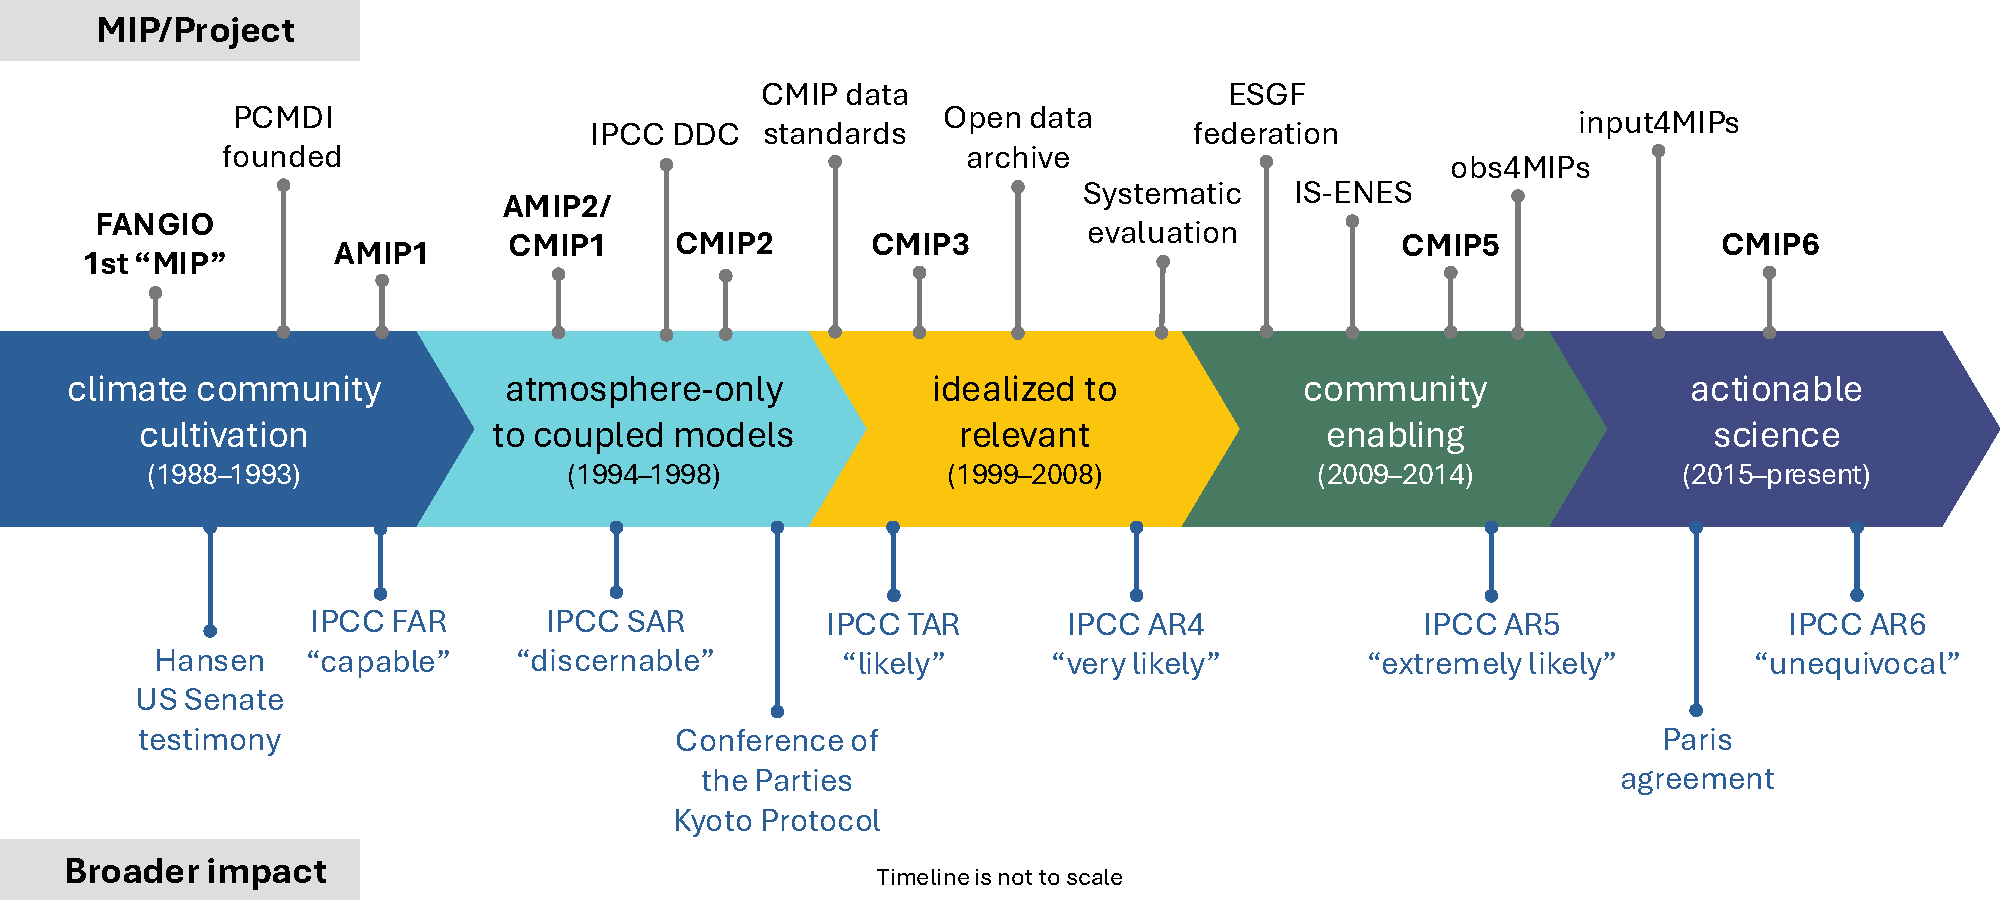
\includegraphics[width=\textwidth]{241126T171500_Fig6.pdf}
    \caption{A time history of MIPs and their broader impact, with particular relevance to the IPCC Assessment Report phases and statements of human influence on the climate (in parentheses, FAR through AR6; see \autoref{sec:amip1And2} through \autoref{sec:cmip6ProjectDesign}).}
    %\cred{ESG I, II, missing, what else?}
    \label{fig:fig6-MIPImpact}
\end{figure*}


An alternative, although similarly imperfect, impact metric is based on data download statistics. Like citation counts, these provide relevant measures of user interest across CMIP phases, across contributing or endorsed participating MIPs, and across their respective experiments. An advantage of download assessment is that it should capture interest outside the academic community, which may be less inclined to record its use of data through peer-reviewed publications. Before CMIP3, however, no data download records are available, which limits a comprehensive assessment. An additional complexity is that direct comparison across phases is impossible due to the marked increase in activities and experiments over time (see \autoref{tab:tab1-MIPsThroughTime}, \autoref{tab:tabAppA1-MIPExperiments}).

Like the literature citations, a clear picture emerges when the download data is assessed comparably across phases (\autoref{fig:fig5-MIPDownloads}). These show an evident repeating dominance of three key experiments, the CMIP/DECK 20C3M/historical (dark orange) and piControl (light orange), and all flavours of the ScenarioMIP experiments (which have been cumulatively pooled, red; CMIP3: 3 SRES; CMIP5: 4 RCPs; and CMIP6: 8 SSPs) dominating downloads. For each of the successive phases, 6 of 12 CMIP3 experiments account for 94.3\% of downloads (top), 10 of 37 CMIP5 experiments account for 90.3\% (middle), and 16 of 322 CMIP6 experiments account for 90.7\% of downloads (bottom). Considering only the top three experiments across phases (with the downloads of all ScenarioMIP experiments pooled), these account for 89\%, 80\%, and 76\% of the total downloads for CMIP3, CMIP5, and CMIP6, respectively. A similar assessment can be made when considering the same download records grouped across activities, with CMIP/DECK and ScenarioMIP again dominating totals (\autoref{fig:figA1-MIPDownloads}).

In an attempt to document the broader climate science impact, chronologically aligned with the MIP phases, \autoref{fig:fig6-MIPImpact} displays an approximate time-history of MIP activities and other milestones noted in earlier sections, along with the IPCC assessment attribution statements and international agreements that were made. For each IPCC assessment, the calibrated language likelihood scale \citep[e.g.,][]{mastrandrea_guidance_2010} assessment of human influence on climate is noted, beginning with ``humankind is \textit{capable} of raising the global-average annual-mean surface-air temperature'' in FAR \citep{ipcc_policymakers_1990} through to the definitive ``It is \textit{unequivocal} that human influence has warmed the atmosphere, ocean and land'' in AR6 \citep{ipcc_summary_2021}.

There is sometimes confusion regarding the relationship between CMIP and the IPCC assessments, with some thinking that CMIP and IPCC are interchangeable or that CMIP is somehow ``run'' by the IPCC. This is, of course, not the case. CMIP (and AMIP before it) was formulated as a scientific research activity whereby the modelling groups performing present-day and future climate simulations could intercompare their results to advance understanding of the climate system and publish their findings in peer-reviewed scientific papers. The IPCC assessments depended directly on the papers emerging from the CMIP phases to formulate periodic updates of the current understanding of climate variability and change. However, as the IPCC assessments grew in importance, the modelling groups participating in CMIP were aware of the IPCC process, which motivated, in part, their participation in CMIP and determined the timelines established for each of the latter CMIP phases (CMIP5, CMIP6). Thus, a symbiotic relationship developed between CMIP and the IPCC assessments \citep{meehl_role_2023}. However, without CMIP, the IPCC assessments could not have been possible. Without the coordinated community climate science efforts embodied by the AMIP and CMIP phases, progress in Earth's climate understanding would not have advanced to our present state of knowledge.

\mycomment{
%%##### COMMENTS %#####
CMIP6 30 data nodes publishing data, 9 reporting download statistics
CMIP5 $\sim$35 data nodes publishing, 7 reporting download statistics (all CMIP6 data nodes)
%#####
}


\section{CMIP phase 6 completion}
\label{sec:CMIP6Completion}

The CMIP6 project is now mostly complete, with nearly all CMIP modelling groups prioritizing ongoing model development over running CMIP6 simulations. Consequently, the growth of the ESGF CMIP6 archive has markedly slowed (see \autoref{fig:fig2-CMIP6DataGrowth}).

CMIP has realized the potential of open-access data, enabling science discovery and reproducibility. It has become a de facto standard and an umbrella project for the distributed special-interest Community MIPs to organize their science and cross-institutional collaborations. More generally, the CMIP-supporting infrastructure is increasingly being relied upon to facilitate and enable coordinated climate science. Any CMIP-contributing modelling group can design an experimental protocol to address some scientific question and, through existing relationships and connections, engage like-minded researchers in collaborating modelling centres to tackle the problem using a multi-model framework \citep[e.g.][]{jones_bringing_2024}.

After nearly all CMIP6 simulation results had been published and the IPCC AR6 had been published, the WGCM and the CMIP and WIP Panels undertook a CMIP6 survey to assess project success and gather community feedback \citep{orourke_cmip6_2024}. For the CMIP-supporting infrastructure, this survey identified some clear priorities, acknowledging CMIP6 progress, but calling for further improvements. In particular, it called for the ``CMIP framework'', including all supporting infrastructure (see \autoref{sec:CMIPSupportingOrgsAndInfra}, and \autoref{sec:CMIP6SupportingProjects}) to be maintained and made available in an ongoing capacity, so that this building infrastructure could continue to serve the growing CMIP contributor and downstream user communities.

An interim phase, CMIP6Plus, was initiated to address this need and expand the now well-established data standardisation requirements, data-sharing culture, and collaborative goodwill proven essential to CMIP's success \citep{mizielinski_cmip6plus_2024}. The project, led by the WIP, has continued to develop the underlying infrastructure responsible for delivering CMIP6, adapting and modularising it to enable ongoing use with limited additional technical investments by contributing modelling groups or MIP leads. The goal has been to establish consistent data requirements and a sound supporting infrastructure serving to minimise data preparation and publication efforts and enhance scientific productivity and impact. This allows several CMIP6 follow-on activities to continue leveraging the infrastructure in the service of climate science research. The project provides ongoing, but limited support for coordinated model experimentation.

Planning for the 7th phase of CMIP (CMIP7) has now begun with an emphasis on broad community consultation \citep{orourke_cmip6_2024}. As discussions continue on the core science foci of CMIP7 \citep[e.g.,][]{dunne_climate_2023,dunne_evolving_2024}, CMIP infrastructure providers are undertaking work \citep[e.g.,][]{kershaw_esgf_2020} to modernise and ready services for a relatively small number of CMIP7 AR7 ``Fast Track'' experiments, which are expected to begin in mid-2025 \citep{dunne_evolving_2024}. At that time, new additions to the CMIP6 data archive will cease, and the next-generation simulations based on the latest model versions, updated forcing datasets (\autoref{sec:CMIP6SupportingProjects-input4MIPs}), and refined experimental protocols may begin to be published.

\mycomment{
%%##### COMMENTS %#####
MIP6Plus: Infrastructure concepts of multiverse/CMIP, planet/project, and continent/usernodes)
%#####
}


\section{CMIP phase 7 planning}
\label{sec:CMIP7Planning}
\cite{mizielinski_cmip6_2025, juckes_baseline_2025}


\section{Summary} %% \conclusions[modified heading if necessary]
\label{sec:Summary}

CMIP6 is the latest in a long history of internationally coordinated and scientifically collaborative climate model-based research projects. CMIP has developed standard approaches to evaluate and intercompare climate models and a standardised vocabulary and infrastructure for defining and delivering data to a broad and expanding community. It has ensured that projections of future climate conditions are based on a robust and consistent framework.

It has now been 35 years since a group of experts with an interest in modelling standards and climate model intercomparison met informally in Boulder, Colorado, a meeting that led to the first MIP, AMIP1 \citep{gates_amip_1991}. Since then, MIPs have captivated and engaged a broad and growing number of researchers who have had a tangible impact in improving our knowledge of Earth's climate system.

CMIP has generated profound scientific insights that define how we understand and address climate change and our ability to quantify and attribute the drivers and responses to the observed climate changes we are experiencing today. It has improved climate prediction, provided quantified insights that guide policy and decision making, informed risk and adaptation strategies and climate change mitigation planning, and improved public awareness and climate education. Its contributions have touched almost every aspect of society and raised awareness of the urgent need for global action on climate change.

Although the project has been a demonstrable success with its focus on the dual goals of facilitating cutting-edge climate research and delivering climate data that enable a broad array of downstream activities, CMIP's growth and broadening community expectations have strained existing resources traditionally devoted to the priorities of modelling centre research staff. There is some concern that the value of CMIP in meeting the climate information needs of those outside the research community is draining research funds that might be used more productively to develop better models and carry out innovative research. This pressure is not new. After CMIP3, there were calls for a reformulation of efforts to centralize resources across contributors to produce very high-resolution, regionally relevant climate predictions \citep{shukla_strategies_2009,shukla_toward_2010}. Somewhat similar calls have been repeated near the end of this most recent CMIP6 phase \citep{jakob_need_2023,stevens_perspective_2024}.

Although modelling groups continue to shoulder most of the responsibility for CMIP, the WCRP created in March 2022 a CMIP International Project Office (CMIP-IPO) funded and hosted by the European Space Agency (ESA, UK) to assist the CMIP Panel and the WIP in coordinating the project. The CMIP-IPO is tasked with supporting the design and development of the upcoming CMIP7 project (see \href{https://wcrp-cmip.org/cmip7}{https://wcrp-cmip.org/cmip7}) and facilitating broad and growing engagement of individuals that might participate in it and benefit from its results. CMIP7 is expected to meet the needs of the IPCC AR7 cycle through a continued federation of activities that will benefit from the lessons learned in CMIP6 \citep{eyring_overview_2016}. Efforts will be made to reduce modelling group burdens by better consulting the broad community, clarifying needs, and apportioning the limited resources to meet them. 

The CMIP project has had a sustained global impact. Its success has depended on the efforts of tenacious individuals or small teams that encouraged and facilitated initial community engagement. These initial steps, coupled with the coordinated efforts within and across modelling groups, the infrastructure providers, and other contributors, led to the broad community collaboration and coordination which resulted in CMIP's ongoing impact. At its core, the project is a fundamental anchor point of international climate research, facilitating the generation of climate simulations of value to research and climate change planning. In return, modelling groups benefit from coordinated, collaborative activities and community evaluation, which feed back on the climate model development process, suggesting that indeed ``intercomparison makes for a better climate model.''


%% Following commands are statements for data sets and/or software code availability corresponding to the manuscript.
%% Use these sections if data sets and/or software code are part of what your research article is based on.

%\codeavailability{TEXT} %% use this section when having only software code available

%\dataavailability{TEXT} %% use this section when having only data sets available

\codedataavailability{
Data and code supporting the figures and tables in this paper are available via GitHub at \url{https://github.com/durack1/CMIPSummary}, or viewed directly at \url{https://nbviewer.org/github/durack1/CMIPSummary/blob/main/figuresAndTables.ipynb}. A persistent Zenodo archive is also available at {https://doi.org/10.5281/zenodo.15321348}.
} %% use this section when having data sets and software code available

\mycomment{OLD TEXT: Data underpinning figures in the paper, in addition to tabulated additional information, can be viewed in a paper-dedicated GitHub repository at \url{https://github.com/durack1/CMIPSummary}, or using NBViewer at \url{https://nbviewer.org/github/durack1/CMIPSummary/blob/main/figuresAndTables.ipynb}. All code and materials are also accessible in a Zenodo archive, accessible at \url{https://doi.org/10.5281/zenodo.15321348}.}

%\sampleavailability{TEXT} %% use this section when having geoscientific samples available

%\videosupplement{TEXT} %% use this section when having video supplements available

\appendix
\section{Defined experiments across MIP phases}  %% Appendix A
%\subsection{}     %% Appendix A1, A2, etc.
\label{sec:secAppA1-MIPExperiments}
There is considerable continuity with experimental protocols across phases. The ``amip'' AGCM experiment is where MIP science began, covering the 1979-1988 period for AMIP1, and 1979-2001 for AMIP2. The concept of a fixed climatological forced ``control'' experiment identified core experiments between CMIP1 and CMIP2, with the present-day control (pdcntrl, $\sim$1995 CMIP1) evolving to include a pre-industrial control (picntrl, $\sim$1850-1860 CMIP2) in subsequent phases. When assessing the ``control'' experiments, the nomenclature changed a little, with picntrl (before CMIP5) and piControl referring to the same experimental protocols, noting differing ``pre-industrial'' climatological fixed forcings were used across phases (see \autoref{sec:CMIP6SupportingProjects-input4MIPs}). Idealized experiments were also incorporated in CMIP2, with the 1\% compounding (1pctCO2) first included and subsequently identified as 1pctto2x and 1pctto4x (before CMIP5), returning to the single 1pctCO2 identity in CMIP5 onward, and with differing simulation lengths across contributing models (2x 70 years, and 4x 140 years). The historical experiment, with transient time-evolving forcings included, was first defined in CMIP3, identified as 20C3M (climate of the twentieth century, $\sim$1860-1999). This is subsequently the historical experiment (CMIP5 and onward) and was extended to include additional forcing coverage (CMIP5: 1850-2011; CMIP6: 1850-2014). For further details and comparisons, see \autoref{tab:tabAppA1-MIPExperiments}, and to visualize the experiment growth over phases, see \autoref{fig:fig1-MIPGrowth}.

\begin{table*}[htp]
	\renewcommand{\arraystretch}{1.5}
	\scriptsize
	\centering
	\caption{MIP Experiments AMIP1 (1991) through CMIP6}
	\resizebox{\textwidth}{!} {
		\begin{tabularx}{0.9\textwidth} {
				| >{\centering\arraybackslash\hsize=.08\hsize}X
				| >{\centering\arraybackslash\hsize=.2\hsize}X
				| >{\centering\arraybackslash\hsize=.46\hsize}X
				| >{\centering\arraybackslash\hsize=.26\hsize}X | }
			\hline
			\textbf{MIP Phase} & \textbf{Citation/Year} & \textbf{Experiment(s)} & \textbf{URL/DOI}\\ \hline
			AMIP1 & \citet{gates_amip_1991} & \textbf{AMIP:} amip & \href{http://doi.org/10.5281/zenodo.12109765}{10.5281/zenodo.12109765}; \url{https://web.archive.org/web/19970524094021/http://www-pcmdi.llnl.gov/amip/}\\ \hline
			AMIP2 & \citet{gleckler_amip_1999} & \textbf{AMIP:} amip & \href{http://doi.org/10.5281/zenodo.12188729}{10.5281/zenodo.12188729}; \url{https://web.archive.org/web/19970524094021/http://www-pcmdi.llnl.gov/amip/}\\ \hline
			CMIP1 & \citet{meehl_global_1995} & \textbf{CMIP:} pdcntrl & \url{https://web.archive.org/web/19970824235843/http://www-pcmdi.llnl.gov/cmip/Cmip.htm}\\ \hline
			CMIP2 & \citet{meehl_intercomparison_1997} & \textbf{CMIP:} pdcntrl, picntrl, 1pctCO2 & \url{https://web.archive.org/web/19970825000210/http://www-pcmdi.llnl.gov/cmip/announ.htm}\\ \hline
			CMIP3 & Doutriaux \& Taylor, 2005; \citet{meehl_wcrp_2007} & \textbf{CMIP:} 1pctto2x, 1pctto4x, 20C3M, amip, pdcntrl, picntrl; \textbf{CFMIP:} 2xco2, slabcntl; \textbf{ScenarioMIP:} commit, SRESA1B, SRESA2, SRESB1 & \url{https://pcmdi.llnl.gov/mips/cmip3/experiment.html\#Experiments}\\ \hline
			CMIP5 & \cite{taylor_cmip5_2011,taylor_overview_2012}; Doutriaux \& Taylor, 2013 & \textbf{CMIP:} 1pctCO2, abrupt4xCO2, amip, historical, piControl; \textbf{C4MIP:} esmControl, esmFdbk1, esmFdbk2, esmFixClim1, esmFixClim2, esmHistorical, esmrcp85; \textbf{CFMIP:} amip4K, amip4xCO2, amipFuture, aqua4K, aqua4xCO2, aquaControl, sst2030 \textbf{DCPP:} decadalXXXX, noVolcXXXX, volcIn2010; \textbf{DAMIP:} historicalExt, historicalGHG, historicalMisc, historicalNat; \textbf{PMIP:} lgm, midHolocene, past1000; \textbf{RFMIP:} sstClim, sstClim4xCO2, sstClimAerosol, sstClimSulfate; \textbf{ScenarioMIP:} rcp26, rcp45, rcp60, rcp85 & \url{https://pcmdi.llnl.gov/mips/cmip5/experiment\_design.html}\\ \hline			
			CMIP6 & \citet{eyring_overview_2016}; \citet{durack_cmip6_2024} & $\sim$190 (2016) to 322 (2024) see CMIP6\_CVs; for MIPs contributing to the phase see \autoref{tab:tab2-CMIP6MIPs} & \href{http://doi.org/10.5281/zenodo.12197150}{10.5281/zenodo.12197150}; \url{https://github.com/WCRP-CMIP/CMIP6\_CVs}; \url{https://wcrp-cmip.github.io/CMIP6\_CVs/docs/CMIP6\_experiment\_id.html}\\
			\hline		
		\end{tabularx}
	} % /resizebox
	\label{tab:tabAppA1-MIPExperiments}
	\footnotesize{Notes: For CMIP3 and CMIP5, no ``Endorsed-MIPs'' were identified, rather experiments were included without recognizing the community that defined these experiments. To attempt to provide connectivity across CMIP phases, CMIP6-era MIP identities (see \autoref{tab:tab2-CMIP6MIPs}, e.g., CFMIP, ScenarioMIP) have been retrofitted back to prior phase experiments which led to corresponding experiments in CMIP6. In CMIP5, NOAA-GFDL submitted GFDL-HIRAM-C180 simulations for the CFMIP-motivated sst2090 and sst2090rcp45 experiments (as these were single model experiments they are not listed above).}
    % Mappings see Taylor google doc XML filename construction https://docs.google.com/document/d/1bUwK6G_fVZO53UjLZbQUOuBP47PsT8lqKKhL1pjRnKg/edit
    %\cred{Numbers are calculated in an Excel spreadsheet for the early text or web-based lists.} 
\end{table*}


\begin{figure*}
    \centering
    \includesvg[width=\textwidth]{250501T214501_FigA1.svg}
    \caption{Recorded downloads across the three phases of CMIP, for which download records are available, following \autoref{fig:fig5-MIPDownloads}. Left the top 6 CMIP3 experiment downloads across the 12 experiments that defined phase \citep{meehl_wcrp_2007}. Middle the CMIP5 downloads for the top 4 MIPs of the 8 that defined the phase \citep[\autoref{tab:tabAppA1-MIPExperiments};][]{taylor_overview_2012}. And right the CMIP6 downloads for the top 4 MIPs of the 22 that defined the phase \cite[[see \autoref{tab:tab2-CMIP6MIPs};][]{eyring_overview_2016}. For CMIP6, almost 45\% of downloads were accounted for by the core CMIP/DECK simulations, and 38\% accounted for in the ScenarioMIP future projection experiments \citep{oneill_scenario_2016}. This pattern of data download priority is mirrored across the prior phases, with CMIP5 (CMIP 61\%, ScenarioMIP 25\%) and a more dominant 20C3M/picntrl demand in CMIP3 (CMIP 64\%, 35\% ScenarioMIP).}
    \label{fig:figA1-MIPDownloads}
    %\cred{Appetite to tabulate these results?}}.
    %\cred{Sandro F., can these numbers, obtained Nov 2024 be relied upon to represent the full 2010-2018 CMIP5 project downloads?}
\end{figure*}



\section{MIP variable request, standard output and data growth}  %% Appendix B
\label{sec:secAppB1-MIPStandardOutput}
The information presented in \autoref{tab:tab1-MIPsThroughTime} row ``Standard output variables/Tables'' was collated from numerous live and archived resources available from 1991 through to the CMIP6 CMOR Table files that are still being used today. The earliest resources were published in written form, the AMIP Newsletters \citep[e.g.,][]{gates_amip_1991}, and subsequently, became available on the PCMDI website for AMIP2, CMIP1 and CMIP2/2+ phases. CMIP3 marked a step change, with the development of the CMOR1 software \citep{taylor_cmor_2006} and CMIP3 Standard Output defined by the more complete CMIP3-CMOR-Tables \citep{doutriaux_cmip3_2005}. CMIP5 continued this trend with CMOR2 \citep{doutriaux_cmor_2011} and the CMIP5-CMOR-Tables \citep{doutriaux_cmip5_2013}. For CMIP6, project expansion to include 22 MIPs and 322 experiments (\autoref{tab:tab2-CMIP6MIPs}, \autoref{tab:tab1-MIPsThroughTime} respectively) required the development of a dedicated CMIP6 Data Request (see \autoref{sec:CMIP6DR}) along with the parallel development of CMOR3 \citep{mauzey_cmor_2024} and the CMIP6-CMOR-Tables \citep{nadeau_cmip6_2017}, themselves built from the CMIP6 Data Request \citep{juckes_cmip6_2020}. For each tabulated value, superscript-identified links provide live connections to these sources, see \autoref{tab:tabAppB1-MIPStandardOutput}.


% Rerun https://github.com/durack1/Duracketal24-CMIP6/blob/main/getVarCounts.py against other table sets to fill in numbers below
\begin{table*}[htp]
	\renewcommand{\arraystretch}{1.5}
	\scriptsize
	\centering
	\caption{MIP variable request and standard output AMIP1 (1991) to CMIP6}
	\resizebox{\textwidth}{!} {
		\begin{tabularx}{0.9\textwidth} {
				| >{\centering\arraybackslash\hsize=.09\hsize}X
				| >{\centering\arraybackslash\hsize=.07\hsize}X
				| >{\centering\arraybackslash\hsize=.07\hsize}X
				| >{\centering\arraybackslash\hsize=.07\hsize}X
				| >{\centering\arraybackslash\hsize=.1\hsize}X
				| >{\centering\arraybackslash\hsize=.6\hsize}X | }
			\hline
			\textbf{Table 1 superscript} & \textbf{MIP Phase} & \textbf{Variable Count} & \textbf{CMOR version} & \textbf{Citation/Year} & \textbf{URL/DOI}\\ \hline
			1 & AMIP1 & 32 & $\sim$ & \citet{gates_amip_1991} & \href{http://doi.org/10.5281/zenodo.12109765}{10.5281/zenodo.12109765}; \url{https://pcmdi.llnl.gov/mips/amip/OUTPUT/WGNEDIAGS/index.html}\\ \hline
			2 & AMIP2 & 114 & $\sim$ & 1998 & \url{https://pcmdi.llnl.gov/mips/amip/OUTPUT/AMIP2/outlist.html}\\ \hline
			3 & CMIP1 & 23 & $\sim$ & 1997 & \url{https://web.archive.org/web/19970824233750/http://www-pcmdi.llnl.gov/cmip/diagsub.html}\\ \hline
			4 & CMIP2 & 28 & $\sim$ & 1997 & \url{https://pcmdi.llnl.gov/mips/cmip2/}\\ \hline
			5 & CMIP3 & 143\textsuperscript{\textdagger} & 1.0 & Doutriaux \& Taylor, 2005 & \href{http://doi.org/10.5281/zenodo.12792173}{10.5281/zenodo.12792173}; \url{https://github.com/PCMDI/cmip3-cmor-tables}\\ \hline
			6 & CMIP5 & 986 & 2.0 & Doutriaux \& Taylor, 2013 & \href{http://doi.org/10.5281/zenodo.12792191}{10.5281/zenodo.12792191}; \url{https://github.com/PCMDI/cmip5-cmor-tables}\\ \hline
			7 & CMIP6 & 2062 & 3.0 & Nadeau et al., 2018; \citep{juckes_cmip6_2020, juckes_baseline_2025} & \href{http://doi.org/10.5281/zenodo.597650}{10.5281/zenodo.597650}; \url{https://github.com/PCMDI/cmip6-cmor-tables}\\ \hline
			\hline
			$\sim$ & CFMIP1 & 149 & 1.0 & $\sim$ & \url{https://github.com/PCMDI/cfmip1-cmor-tables}\\ \hline
			$\sim$ & C-LAMP1 & 88 & 1.0 & $\sim$ & \url{https://github.com/PCMDI/c-lamp1-cmor-tables}\\ \hline
			$\sim$ & IAEMIP1 & 146 & 1.0 & $\sim$ & \url{https://github.com/PCMDI/iaemip1-cmor-tables}\\ \hline
			$\sim$ & CORDEX (CMIP5) & 207 & 2.0 & $\sim$ & \url{https://github.com/PCMDI/cordex-cmor-tables}\\ \hline
			$\sim$ & GEOMIP & 1142 & 2.0 & $\sim$ & \url{https://github.com/PCMDI/geomip-cmor-tables}\\ \hline
			$\sim$ & LUCID & 979 & 2.0 & $\sim$ & \url{https://github.com/PCMDI/lucid-cmor-tables}\\ \hline
			$\sim$ & PMIP3 & 810 & 2.0 & \citet{braconnot_paleoclimate_2011} & \url{https://github.com/PCMDI/pmip3-cmor-tables}\\ \hline
			$\sim$ & CORDEX-CMIP6 & 565 & 3.0 & \citet{gutowski_jr_wcrp_2016} & \url{https://github.com/WCRP-CORDEX/cordex-cmip6-cmor-tables}\\
			\hline
		\end{tabularx}
	} % /resizebox
	\label{tab:tabAppB1-MIPStandardOutput}
	\footnotesize{Notes: {}\textsuperscript{\textdagger}In the CMIP3 phase, the total defined A5 table variables were 4, both adjusted/instantaneous shortwave forcing and its clearsky equivalent. This differs from the 223 identities in the table, which identified similar quantities (either top of atmosphere or tropopause, and variations due to unique forcing, e.g., all greenhouse gases, carbon dioxide only, total sulphate aerosol, direct effect only of sulphate aerosol, indirect effect only of sulphate aerosols, ``black carbon'', ozone, tropospheric ozone only, stratospheric ozone only, vegetation and other land surface changes, all anthropogenic factors, inclusive, volcanic aerosols, solar constant changes, all-natural factors inclusive.}
\end{table*}


\begin{figure*}
    \centering
    \includesvg[width=\textwidth]{250501T214501_FigB1.svg}
    \caption{Data growth across all MIP phases, AMIP1 1989 through CMIP6 today. This figure is a visual representation of tabulated data volumes in \autoref{tab:tab1-MIPsThroughTime}. Note a y-axis log-scale, capturing data growth from gigabytes/10$^9$ bytes for AMIP1 and CMIP1 through to the tens of petabyte/10$^{15}$ bytes scale in CMIP6.}
    \label{fig:figB1-MIPDataGrowth}
\end{figure*}


\section{MIP errata}  %% Appendix C
\label{sec:secAppC1-MIPErrata}
Tabulated entries of CMIP errata based on phase, see \autoref{tab:tabAppC1-MIPErrata}.

\begin{table*}[htp]
	\renewcommand{\arraystretch}{1.5}
	\scriptsize
	\centering
	\caption{MIP Errata CMIP3 (2004) to CMIP6}
	\resizebox{\textwidth}{!} {
		\begin{tabularx}{0.9\textwidth} {
				| >{\centering\arraybackslash\hsize=.1\hsize}X
				| >{\centering\arraybackslash\hsize=.25\hsize}X
				| >{\centering\arraybackslash\hsize=.65\hsize}X | }
			\hline
			\textbf{MIP Phase} & \textbf{Errata count (reporting period)} & \textbf{URL/DOI}\\ \hline
			CMIP3 & 122 (2004-2011) & \url{http://web.archive.org/web/20150906073117/https://esg.llnl.gov:8443/about/errata.do}\\ \hline
			CMIP5 & 84 (2012-2015) & \url{https://pcmdi.llnl.gov/mips/cmip5/errata.html}\\ \hline
			CMIP6 & 462 (2018-2024) & \url{https://errata.ipsl.fr}\\
			\hline
		\end{tabularx}
	} % /resizebox
	\label{tab:tabAppC1-MIPErrata}
	\footnotesize{Notes: All values are tabulated from archived or live webpages as of 28$^{th}$ November, 2024.}
    %\DTMsetstyle{en-GB}\DTMnow
\end{table*}

\mycomment{
%%##### COMMENTS %#####
What do we need DOI'd - can zenodo work?
CMIP2: https://pcmdi.llnl.gov/mips/cmip2/
CMIP3: https://pcmdi.llnl.gov/mips/cmip3/experiment.html
CMIP5: https://pcmdi.llnl.gov/mips/cmip5/requirements.html
standard_output doc - with coverpage (Karl)
ODS2.5: Gleckler et al. 2024 https://docs.google.com/document/d/1bTi5-CKR8xBCA4e3egc4FXJ93LuUfrhyEBHpUCVgZuo/edit
Also Potter et al. 2011 https://doi.org/10.1175/2011BAMS3018.1
%#####
}


\section{\cred{CMIP download statistics}}  %% Appendix D
\label{sec:secAppD1-CMIPDownloads}

\cred{\textbf{Some info about download stats}}
%% Alessandra and Fabrizio have provided details in
% https://docs.google.com/document/d/1xum5wePapEC0m1ER-ind5NtY2zsc4MbiuX5ryYGwXus/edit?tab=t.0

\begin{table*}[htp]
\renewcommand{\arraystretch}{2}
\scriptsize
\centering
\caption{Download statistics, their source, temporal coverage, and web resource (if available)}
\resizebox{\textwidth}{!} {
	\begin{tabularx}{1\textwidth} { 
	  | >{\raggedright\arraybackslash\hsize=.1\hsize}X
	  | >{\centering\arraybackslash\hsize=.15\hsize}X
	  | >{\centering\arraybackslash\hsize=.225\hsize}X
	  | >{\centering\arraybackslash\hsize=.5\hsize}X
    | >{\centering\arraybackslash\hsize=.1\hsize}X }
\hline
\textbf{MIP Phase} & \textbf{Temporal coverage} & \textbf{Source} & \textbf{URL} \\ \hline
CMIP3 & 2004-2008 & PCMDI, LLNL (Archive) & - \\ \hline
CMIP5 & 2012-2017;\newline 2018- & CMCC (Archive);\newline CMCC (Live web) & -\newline\url{https://esgf-ui.cmcc.it/esgf-dashboard-ui/cmip5.html} \\ \hline
CMIP6 & 2018- & CMCC (Live web) & \url{https://esgf-ui.cmcc.it/esgf-dashboard-ui/cmip6.html} \\ \hline
\end{tabularx}
} % /resizebox
\label{tab:secAppD1-CMIP6Downloads}
\footnotesize{}
\end{table*}








\section{\cred{CMIP downstream data services and analysis tools}}  %% Appendix E
\label{sec:secAppE1-CMIPDownstreamServices}

\cred{The sustained CMIP development across multiple phases, along with publicly open data access since CMIP3 \autoref{sec:cmip3}, facilitated the development of numerous downstream tools, and data services which repackage and reformulate CMIP output for science use. In addition, non-ESGF data repositories are also now available, facilitating broad data access. A non-exhaustive list of several examples is included in \autoref{tab:secAppE1-CMIP6DownstreamServices}. In addition to data sources, the stability of the CMIP netCDF data format which was first established in CMIP3 has allowed for the development of numerous analysis packages and evaluation tools to be developed (see also \autoref{sec:CMIP6SupportingProjects-CoordEval}), facilitating reproducible CMIP model analysis and evaluation, numerous examples are listed at \url{https://wcrp-cmip.org/tools}.}

\begin{table*}[htp]
\renewcommand{\arraystretch}{2}
\scriptsize
\centering
\caption{Downstream data services, in addition to the federated ESGF nodes, facilitated by the publicly open data access model, first defined in CMIP3 (non-exhaustive list)}
\resizebox{\textwidth}{!} {
	\begin{tabularx}{0.9\textwidth} { 
	  | >{\raggedright\arraybackslash\hsize=.25\hsize}X
	  | >{\centering\arraybackslash\hsize=.2\hsize}X
	  | >{\centering\arraybackslash\hsize=.3\hsize}X
	  | >{\centering\arraybackslash\hsize=.1\hsize}X
	  | >{\centering\arraybackslash\hsize=.15\hsize}X | }
\hline
\textbf{Project or package} & \textbf{CMIP phase data available} & \textbf{URL} & \textbf{Citation} & \textbf{DOI}\\ \hline
KNMI Climate Explorer & CMIP3, CMIP5, CMIP6, plus others & \url{https://climexp.knmi.nl} & \cite{trouet_knmi_2013} & - \\ \hline
PANGEO & CMIP3, CMIP5, CMIP6 & \url{https://pangeo-data.github.io/pangeo-cmip6-cloud} & \cite{abernathey_cmip6_2020} & - \\ \hline
Copernicus Climate Change Service (C3S) & reformatted CMIP5, CMIP6 & \url{https://cds.climate.copernicus.eu/datasets?q=CMIP} & - & - \\ \hline
IAC ETHZ & CMIP2, CMIP3, CMIP5, CMIP6 & \url{https://data.iac.ethz.ch/atmos} & - & - \\ \hline
IPCC CMIP6 Interactive Atlas & CMIP6 & \url{https://interactive-atlas.ipcc.ch} & \cite{gutierrez_atlas_2021} & 10.1017/ 9781009157896.021 \\ \hline
CORDEX &  Downscaled CMIP5, CMIP6 & \url{https://cordex.org/} & \cite{jones_coordinated_2011,gutowski_jr_wcrp_2016} & - \\ \hline
The U.S. Climate Resilience Toolkit CLIMATE EXPLORER & Downscaled CMIP5 & \url{https://crt-climate-explorer.nemac.org} & - & - \\ \hline
NOAA’s Climate Projection Web Portal & Downscaled CMIP5 and others & \url{https://psl.noaa.gov/ipcc} & - & - \\ \hline
NASA CMIP5: 21st Century Temperature and Precipitation Scenarios & Visualized CMIP5 future scenarios & \url{https://svs.gsfc.nasa.gov/4110} & - & - \\ \hline
World Bank Climate Projections & CMIP5 future scenarios & \url{https://climateknowledgeportal.worldbank.org/cmip5} & - & - \\ \hline
Climate Information & CMIP5, CMIP6, plus others & \url{https://climateinformation.org} & - & - \\ \hline
Microsoft Planetary Computer & CMIP6 downscaled projections, plus others & \url{https://planetarycomputer.microsoft.com} & - & - \\ \hline
\cred{\textbf{Others?}} & - & - & - & - \\ \hline
\end{tabularx}
} % /resizebox
\label{tab:secAppE1-CMIP6DownstreamServices}
\footnotesize{}
\end{table*}









\section{CMIP6 data preparation tools}  %% Appendix F
\label{sec:secAppF1-CMIP6DataPrep}

During MIP phases, several software tools have been developed and updated to meet augmented phase requirements. These tools build on the MIP nomenclature and digital formats that are now standard. Some prominent packages are tabulated below (see \autoref{tab:secAppF1-CMIP6DataPrep}).

\begin{table*}[htp]
\renewcommand{\arraystretch}{2}
\scriptsize
\centering
\caption{Software packages developed to aid MIP dataset production (non-exhaustive list)}
\resizebox{\textwidth}{!} {
	\begin{tabularx}{0.9\textwidth} { 
	  | >{\raggedright\arraybackslash\hsize=.14\hsize}X
	  | >{\centering\arraybackslash\hsize=.2\hsize}X
	  | >{\centering\arraybackslash\hsize=.46\hsize}X
	  | >{\centering\arraybackslash\hsize=.1\hsize}X
	  | >{\centering\arraybackslash\hsize=.1\hsize}X | }
\hline
\textbf{Software name and version} & \textbf{Software Description} & \textbf{URL} & \textbf{Citation} & \textbf{DOI}\\ \hline
CMOR 1.0 & The Climate Model Output Rewriter & \url{https://cmor.llnl.gov/archive/cmor1}; \url{https://github.com/PCMDI/cmor} & \citet{taylor_cmor_2006} & \href{http://doi.org/10.5281/zenodo.12690071}{10.5281/ zenodo.12690071}\\ \hline
CMOR 2.0 & The Climate Model Output Rewriter & \url{https://cmor.llnl.gov}; \url{https://github.com/PCMDI/cmor} & \citet{doutriaux_cmor_2011} & \href{http://doi.org/10.5281/zenodo.12690366}{10.5281/ zenodo.12690366}\\ \hline
CMOR 3.0 & The Climate Model Output Rewriter & \url{https://cmor.llnl.gov}; \url{https://github.com/PCMDI/cmor} & \citet{doutriaux_cmor_2024} & \href{http://doi.org/10.5281/zenodo.592733}{10.5281/ zenodo.592733}\\ \hline
XIOS & Xml IO Server & \url{http://forge.ipsl.jussieu.fr/ioserver/chrome/site/XIOS\_DOC} & &\\ \hline
ECE2CMOR3 & EC-Earth to CMOR & \url{https://github.com/EC-Earth/ece2cmor3}; \url{https://github.com/EC-Earth/cmor-fixer} & & \href{http://doi.org/10.5281/zenodo.1051094}{10.5281/ zenodo.1051094}\\ \hline
CDDS 3.0 & The Climate Data Dissemination System & \url{https://github.com/MetOffice/CDDS}; \url{https://metoffice.github.io/CDDS/} & &\\ \hline
CDO CMOR & Climate Data Operators to CMOR & \url{https://code.mpimet.mpg.de/projects/cdo/wiki/CDO\_CMOR\_Operator} & &\\ \hline
NORESM2CMOR & NorESM to CMOR & \url{https://github.com/NorESMhub/noresm2cmor} & &\\ \hline
CCLM2CMOR & COSMO-CLM to CMOR & \url{https://github.com/C2SM-RCM/CCLM2CMOR} & &\\ \hline
FGOALS-g-cmor & FGOALS-g to CMOR & \url{https://github.com/dongli/FGOALS-g-cmor} & &\\ \hline
PRIMAVERA & HadGEM to CMOR & \url{https://github.com/goord/cmor} & &\\ \hline
E3SM\_To\_CMIP 1.11.3 & DoE-E3SM to CMOR & \url{https://github.com/E3SM-Project/e3sm\_to\_cmip} & Asay-Davis et al. (2025) &\\ \hline
ACCESS MOPPeR 2.0.0a & A Model Output Post-Processor for the ACCESS climate model & \url{https://github.com/ACCESS-NRI/ACCESS-MOPPeR} & &\\ \hline
pymorize 6.9.32 & A Python based Tool to CMORize NetCDF Data & \url{https://pymorize.readthedocs.io} & Gierz, P. et al. (2025) &\\
\hline
py-cordex 0.9.0 & A Python based Tool to create cordex grids and meta data & \url{https://py-cordex.readthedocs.io} & Buntemeyer, L. (2025) & \href{http://doi.org/10.5281/zenodo.5841741}{10.5281/ zenodo.5841741} \\
\hline

\end{tabularx}
} % /resizebox
\label{tab:secAppF1-CMIP6DataPrep}
\footnotesize{}
\end{table*}


\section{Acronyms}  %% Appendix G
\label{sec:secAppF1-Acronyms}

Over the five decades of MIPs, many acronyms and identifiers have been developed and bled into standard nomenclature. Some of these are used repeatedly throughout the text, and we tabulate entries here (see \autoref{tab:tabAppG1-Acronyms}). Additional identifiers used to describe CMIP6 Community MIPs are detailed in \autoref{tab:tab2-CMIP6MIPs}.

% https://www.overleaf.com/learn/latex/Tables
% https://tex.stackexchange.com/questions/26462/make-a-table-span-multiple-pages
% https://tex.stackexchange.com/questions/376790/tabularx-break-long-tables-over-several-pages
% https://www.overleaf.com/latex/examples/a-longtable-example/xxwzfxkxxjmc
% https://www.math.utah.edu/~golden/resources/Granular_Ice_Paper/Copernicus_Latex_Manual.pdf#page=13
\begin{table*}[htp]
\renewcommand{\arraystretch}{2}
\scriptsize
\centering
\caption{Acronyms used in this manuscript}
\resizebox{\textwidth}{!} {
	\begin{tabularx}{1\textwidth} { 
	  | >{\raggedright\arraybackslash\hsize=.09\hsize}X
	  | >{\centering\arraybackslash\hsize=.91\hsize}X | }
\hline
\textbf{Acronym} & \textbf{Expansion and additional information}\\ \hline
20C3M & CMIP 20th Century Climate in Coupled Models pilot project (now known as the CMIP historical experiment)\\ \hline
AGCI & US Aspen Global Change Institute; \url{https://www.agci.org}\\ \hline
AGCM & Atmospheric General Circulation Model\\ \hline
AMIP & Atmospheric Model Intercomparison Project (also AMIP1 and AMIP2)\\ \hline
ANL & US Argonne National Laboratory; \url{https://www.anl.gov}\\ \hline
AOGCM & Atmospheric and Ocean General/Global Circulation Model\\ \hline
AR4 & IPCC Fourth Assessment Report, 2007; \url{https://www.ipcc.ch/report/ar4/wg1}\\ \hline
AR5 & IPCC Fifth Assessment Report, 2013; \url{https://www.ipcc.ch/report/ar5/wg1}\\ \hline
AR6 & IPCC Sixth Assessment Report, 2021; \url{https://www.ipcc.ch/report/ar6/wg1}\\ \hline
BADC/CEDA & UK British Atmospheric Data Centre (now CEDA; \url{https://www.ceda.ac.uk})\\ \hline
C-LAMP & Carbon-Land Model Intercomparison Project; (now ILAMB; \url{https://www.ilamb.org})\\ \hline
C4MIP & Coupled Climate-Carbon Cycle MIP; \url{https://c4mip.net}\\ \hline
CCSM & NCAR Community Climate System Model; \url{https://www.cesm.ucar.edu/models/ccsm}\\ \hline
CEDA & UK Centre for Environmental Data Analysis; \url{https://www.ceda.ac.uk}\\ \hline
CF & NetCDF Climate and Forecast Metadata Conventions; \url{https://cfconventions.org/}\\ \hline
CFMIP & Cloud Feedbacks MIP (Also CFMIP1, CFMIP2, and CFMIP3; \url{https://www.cfmip.org})\\ \hline
CIESIN & US Center for Integrated Earth System Information (Columbia University); \url{https://sedac.ciesin.columbia.edu/ddc/}\\ \hline
CLIVAR & WCRP Climate Variability and Predictability Core Project; \url{https://www.clivar.org}\\ \hline
CMCC & Italian CMCC Foundation (Euro-Mediterranean Center on Climate Change); \url{https://www.cmcc.it}\\ \hline
CMIP & Coupled Model Intercomparison Project (also CMIP1, CMIP2, CMIP2+, CMIP3, CMIP5, and CMIP6)\\ \hline
CMIP-IPO & UK CMIP International Project Office; \url{https://wcrp-cmip.org}\\ \hline
CMOR & PCMDI Climate Model Output Rewriter (also CMOR1, CMOR2, and CMOR3; \url{https://cmor.llnl.gov/})\\ \hline
COARDS & Cooperative Ocean/Atmosphere Research Data Service conventions\\ \hline
CRU & UK University of East Anglia, Climatic Research Unit; \url{https://www.uea.ac.uk/groups-and-centres/climatic-research-unit}\\ \hline
\multicolumn{2}{l}{\textbf{\autoref{tab:tabAppG1-Acronyms} continued overpage..}}\\
\end{tabularx}
} % /resizebox
\label{tab:tabAppG1-Acronyms}
\end{table*}

% Split table over multiple pages
\addtocounter{table}{-1}
\begin{table*}[htp]
\renewcommand{\arraystretch}{2}
\scriptsize
\centering
\caption{Acronyms used in this manuscript (continued)}
\resizebox{\textwidth}{!} {
	\begin{tabularx}{1\textwidth} { 
	  | >{\raggedright\arraybackslash\hsize=.09\hsize}X
	  | >{\centering\arraybackslash\hsize=.91\hsize}X | }
\hline
CV & Controlled Vocabulary\\ \hline
DandA & climate change Detection and Attribution research\\ \hline
DAMIP & Detection and Attribution MIP\\ \hline
DCPP & Decadal Climate Prediction Project (CMIP6 Community MIP, and WCRP ESMO Working Group; \url{https://www.wcrp-climate.org/dcp-overview})\\ \hline
DECK & Diagnostic, Evaluation and Characterisation of Klima (Core CMIP experiment suite)\\ \hline
DoE & US Department of Energy; \url{https://www.energy.gov}\\ \hline
DOI & Digital Object Identifier; \url{https://www.doi.org}\\ \hline
DKRZ & German Climate Computing Center (Deutsches Klimarechenzentrum; \url{https://www.dkrz.de/en})\\ \hline
DLR & German Deutsches Zentrum f{\"u}r Luft- und Raumfahrt, Institut f{\"u}r Physik der Atmosph{\"a}re; \url{https://www.dlr.de/en}\\ \hline
DRS & Data Reference Syntax\\ \hline
ECMWF & European Centre for Medium-range Weather Forecasts; \url{https://www.ecmwf.int}\\ \hline
ESA & European Space Agency; \url{https://www.esa.int}\\ \hline
ESG & US Earth System Grid (also ESG I, ESG II)\\ \hline
ESG-CET & US Earth System Grid Center for Enabling Technologies\\ \hline
ESGF & Earth System Grid Federation; \url{https://esgf.llnl.gov}\\ \hline
ESM & Earth System Model\\ \hline
ESMValTool & A community diagnostic and performance metrics tool for evaluation and analysis of Earth system Models; \url{https://esmvaltool.org}\\ \hline
ESMO & WCRP Earth System Modelling and Observations Core Project; \url{https://www.wcrp-esmo.org}\\ \hline
FANGIO & Feedback ANalysis of GCMs and In Observations project\\ \hline
FAR & IPCC First Assessment Report, 1990; \url{https://www.ipcc.ch/report/ar1/wg1}\\ \hline
FMI & Finnish Meteorological Institute; \url{https://en.ilmatieteenlaitos.fi}\\ \hline
FTP & File Transfer Protocol (the standard protocol used to transfer files from a server to a client on a network; \url{https://en.wikipedia.org/wiki/File_Transfer_Protocol}\\ \hline
GridFTP & Extension of FTP for grid computing; \url{https://www.globus.org/blog/gridftp-a-brief-history-of-fast-file-transfer}\\ \hline
GAIM & Global Analysis Interpretation and Modeling Task Force (IGBP sub-group)\\ \hline
GARP & International Global Atmospheric Research Program (a precursor to the WCRP; 1967-1982)\\ \hline
\multicolumn{2}{l}{\textbf{\autoref{tab:tabAppG1-Acronyms} continued overpage..}}\\
\end{tabularx}
} % /resizebox
\label{tab:tabAppG1-Acronyms}
\end{table*}

% Split table over multiple pages
\addtocounter{table}{-1}
\begin{table*}[htp]
\renewcommand{\arraystretch}{2}
\scriptsize
\centering
\caption{Acronyms used in this manuscript (continued)}
\resizebox{\textwidth}{!} {
	\begin{tabularx}{1\textwidth} { 
	  | >{\raggedright\arraybackslash\hsize=.09\hsize}X
	  | >{\centering\arraybackslash\hsize=.91\hsize}X | }
\hline
GB & Gigabyte (one billion bytes, 10$^{9}$)\\ \hline
GCM & General/Global Circulation Model\\ \hline
GDT & Gregory, Drach, and Tett conventions; \cite[see][]{gregory_gdt_1999}\\ \hline
GS & Google Scholar citation service; \url{https://scholar.google.com}\\ \hline
HTTP & HyperText Transfer Protocol (the default protocol underlying internet transactions; \url{https://httpwg.org/specs}\\ \hline
IAM & Integrated Assessment Model\\ \hline
IAV & Impacts, Adaptation and Vulnerability research\\ \hline
ICRCCM & Intercomparison of Radiation Codes used in Climate Models project\\ \hline
IGBP & International Geosphere-Biosphere Programme (closed in 2015; \url{http://www.igbp.net}\\ \hline
ILAMB & ORNL International Land Model Benchmarking; \url{https://www.ilamb.org}\\ \hline
IPCC & UN Intergovernmental Panel on Climate Change; \url{https://www.ipcc.ch}\\ \hline
IPCC DDC & IPCC Data Distribution Centre; \url{https://www.ipcc-data.org}\\ \hline
IPO & International Project Office (e.g., CMIP-IPO, \url{https://wcrp-cmip.org/cmip-governance/project-office/}\\ \hline
IPSL & French Institut Pierre-Simon Laplace; \url{https://www.ipsl.fr/en/home-en}\\ \hline
IS-ENES & Infrastructure for the European Network for Earth System Modelling; \url{https://is.enes.org}\\ \hline
JSON & JavaScript Object Notation; text-based format for storing and exchanging data, both human-readable and machine-parseable; \url{https://www.json.org}\\ \hline
LANL & US Los Alamos National Laboratory; \url{https://www.lanl.gov}\\ \hline
LBNL & US Lawrence Berkeley National Laboratory; \url{https://www.lbl.gov}\\ \hline
LLNL & US Lawrence Livermore National Laboratory; \url{https://www.llnl.gov}\\ \hline
MIP & Model Intercomparison Project\\ \hline
NASA & US National Aeronautic and Space Administration; \url{https://www.nasa.gov}\\ \hline
NASA-JPL & US NASA Jet Propulsion Laboratory; \url{https://www.jpl.nasa.gov}\\ \hline
NCAR & US National Center for Atmospheric Research; \url{https://ncar.ucar.edu}\\ \hline
NCI & Australian National Computational Infrastructure; \url{https://nci.org.au}\\ \hline
NERSC & US Department of Energy National Energy Research Scientific Computing Center (formerly the National Energy Research Supercomputer Center); \url{https://www.nersc.gov}\\ \hline
\multicolumn{2}{l}{\textbf{\autoref{tab:tabAppG1-Acronyms} continued overpage..}}\\
\end{tabularx}
} % /resizebox
\end{table*}

% Split table over multiple pages
\addtocounter{table}{-1}
\begin{table*}[htp]
\renewcommand{\arraystretch}{2}
\scriptsize
\centering
\caption{Acronyms used in this manuscript (continued)}
\resizebox{\textwidth}{!} {
	\begin{tabularx}{1\textwidth} { 
	  | >{\raggedright\arraybackslash\hsize=.09\hsize}X
	  | >{\centering\arraybackslash\hsize=.91\hsize}X | }
\hline
NOAA & US National Oceanic and Atmospheric Administration; \url{https://www.noaa.gov}\\ \hline
NOAA-NCEP & US NOAA National Centers for Environmental Prediction; \url{https://www.weather.gov/ncep}\\ \hline
NOAA-PMEL & US NOAA Pacific Marine Environmental Laboratory; \url{https://www.pmel.noaa.gov}\\ \hline
OCMIP & Ocean Carbon-Cycle Model Intercomparison Project; \url{https://www.wcrp-climate.org/modelling-wgcm-mip-catalogue/modelling-wgcm-mips-2/267-modelling-wgcm-catalogue-ocmip}\\ \hline
ORNL & US Oak Ridge National Laboratory; \url{https://www.ornl.gov}\\ \hline
PB & Petabyte (one quadrillion bytes, 10$^{15}$)\\ \hline
PMIP & CMIP Paleoclimate MIP (also PMIP1, PMIP2, PMIP3, and PMIP4; \url{https://pmip.lsce.ipsl.fr})\\ \hline
PMP & PCMDI Metrics Package; \url{https://pcmdi.github.io/pcmdi_metrics}\\ \hline
PCMDI & Program for Climate Model Diagnosis and Intercomparison, LLNL; \url{https://pcmdi.llnl.gov}\\ \hline
P-DRS & PCMDI Data Retrieval and Storage software library \citep[digital format;][]{drach_data_1995}\\ \hline
RCP & Representative Concentration Pathways scenarios (Circa CMIP5)\\ \hline
SAR & IPCC Second Assessment Report, 1995; \url{https://www.ipcc.ch/report/ar2/wg1}\\ \hline
SGGCM & WCRP Steering Group on Global Coupled Models (a precursor to WGCM)\\ \hline
SLCF & short-lived climate forcers\\ \hline
SOLR & Apache SOLR, open-source enterprise-search database; \url{https://solr.apache.org}\\ \hline
SPECTRE & Spectral Radiance Experiment\\ \hline
SRES & IPCC Special Report on Emission Scenarios (Circa CMIP3)\\ \hline
SST & Sea Surface Temperature\\ \hline
TAR & IPCC Third Assessment Report, 2001; \url{https://www.ipcc.ch/report/ar3/wg1}\\ \hline
TB & Terabyte (one trillion bytes, 10$^{12}$)\\ \hline
Unidata & US Unidata Program Center (University Corporation of Atmospheric Research); \url{https://www.unidata.ucar.edu}\\ \hline 
WoS & Clarivate Web of Science Core Collection citation service; \url{https://www.webofscience.com/wos/woscc}\\ \hline
WCRP & World Climate Research Programme; \url{https://www.wcrp-climate.org}\\ \hline
WDAC & WCRP Data Advisory Council (2011-2020; \url{https://www.wcrp-climate.org/data-wdac}\\ \hline
WG1 & IPCC Working Group I (the Physical Science Basis); \url{https://www.ipcc.ch/working-group/wg1}\\ \hline
\multicolumn{2}{l}{\textbf{\autoref{tab:tabAppG1-Acronyms} continued overpage..}}\\
\end{tabularx}
} % /resizebox
\end{table*}

% Split table over multiple pages
\addtocounter{table}{-1}
\begin{table*}[htp]
\renewcommand{\arraystretch}{2}
\scriptsize
\centering
\caption{Acronyms used in this manuscript (continued)}
\resizebox{\textwidth}{!} {
	\begin{tabularx}{1\textwidth} { 
	  | >{\raggedright\arraybackslash\hsize=.09\hsize}X
	  | >{\centering\arraybackslash\hsize=.91\hsize}X | }
\hline
WG2 & IPCC Working Group II (Impacts, Adaptation, and Vulnerability); \url{https://www.ipcc.ch/working-group/wg2}\\ \hline
WG3 & IPCC Working Group III (Mitigation of Climate Change); \url{https://www.ipcc.ch/working-group/wg3}\\ \hline
WGCM & WCRP Working Group on Coupled Modelling; \url{https://www.wcrp-climate.org/ipo-esmo-groups/modelling-wgcm}\\ \hline
WGNE & WCRP Working Group on Numerical Experimentation; \url{https://wgne.net}\\ \hline
WIP & WCRP WGCM Infrastructure Panel; \url{https://www.wcrp-climate.org/wgcm-cmip/wip}\\ \hline
WMGHG & well-mixed greenhouse gases\\ \hline
UN & United Nations; \url{https://www.un.org/en}\\ \hline
US & United States\\ \hline
VIACS AB & Vulnerability, Impacts, Adaptation and Climate Services Advisory Board; \url{https://viacsab.gerics.de}\\ \hline
\end{tabularx}
} % /resizebox
\label{tab:tabAppG1-Acronyms}
\footnotesize{}
\end{table*}


\noappendix  %% use this to mark the end of the appendix section. Otherwise, the figures might be numbered incorrectly (e.g., 10 instead of 1).

%% Regarding figures and tables in appendices, the following two options are possible depending on your general handling of figures and tables in the manuscript environment:

%% Option 1: If you sorted all figures and tables into the text sections, please also sort the appendix figures and appendix tables into the respective appendix sections.
%% They will be correctly named automatically.

%% Option 2: If you put all figures after the reference list, please insert appendix tables and figures after the normal ones.
%% To rename them correctly to A1, A2, etc., please add the following commands in front of them:

\appendixfigures  %% needs to be added in front of appendix figures

\appendixtables  %% needs to be added in front of the appendix tables

%% Please add \clearpage between each table and/or figure. Further guidelines on figures and tables can be found below.



\authorcontribution{P.J.D. outlined the content, completed the initial outline, and shared responsibility for writing the manuscript. K.E.T. assisted in expanding the outline and shared responsibility for writing the manuscript. P.J.G. provided useful feedback on early drafts, which reformulated the outline. G.A.M provided useful context and feedback on \autoref{sec:cmip6InContext} and \autoref{sec:cmip6ProjectDesign}. B.N.L. provided useful context and feedback on \autoref{sec:CFConventions}, \autoref{sec:earthSystemGridFederation}, and \autoref{sec:ModelDocumentation}. C.C. provided useful context and feedback on \autoref{sec:cmip6InContext}. R.J.S. provided useful context and feedback on \autoref{sec:cmip6InContext}. G.L., A.B-N, and S.D. provided useful context and feedback on \autoref{sec:CMIPDataReplication} and \autoref{sec:CMIPErrata}. M.S. provided useful context and feedback on \autoref{sec:IPCC-DDC} and \autoref{sec:DataCitation}. J.G. provided useful context and feedback on \autoref{sec:CFConventions}. M.J. provided useful context and feedback on \autoref{sec:CMIP6DR}. I.T.F. provided useful context and feedback on \autoref{sec:CMIPSupportingOrgsAndInfra}, \autoref{sec:earthSystemGridFederation}, and \autoref{sec:CMIPDataReplication}. All authors contributed to the final version of the manuscript.} %% This section is mandatory
\mycomment{
%%##### COMMENTS %#####
Bryan edits - https://github.com/durack1/CMIPSummary/commit/9a00c06a5adb299cd9aa1295c976773a2b7c0c2c
%#####
}


\competinginterests{All authors declare no competing or conflicting interests. M.S. is a Topic Editor for Geoscientific Model Development.} %% this section is mandatory even if you declare that no competing interests are present

\disclaimer{The views and opinions expressed in this document do not necessarily state or reflect those of the United States Government, the Department of Energy (DoE), or Lawrence Livermore National Laboratory (LLNL). They shall not be used for advertising or product endorsement purposes.} %% optional section

\begin{acknowledgements}

This article is dedicated to W. Lawrence ``Larry'' Gates, the first PCMDI Director, whose vision, leadership, and skill in building community engagement and consensus garnered acceptance for open and systematic climate model analysis and led to the transformative impact of CMIP.

We acknowledge all past and present members of the WGCM Infrastructure Panel (WIP), CMIP Panel, and Earth System Grid Federation (ESGF) and their precedent organizations. Without the collective efforts of these teams, the progress that CMIP embodies would not have been possible. The authors listed in this article represent a tiny subset of the project contributors over time.

We acknowledge all MIP contributing modelling groups, the World Climate Research Programme's (WCRP) Working Group on Coupled Modelling (WGCM) and its WGCM Infrastructure (WIP), and the CMIP Panels for their leadership in defining and delivering multiple CMIP and preceding AMIP phases. The simulation contributions, which now embody petabytes of the latest generation of historical and future climate data, are the tangible substance of the CMIP project across phases.

We acknowledge the Program for Climate Model Diagnosis and Intercomparison (PCMDI, US), the Centre for Environmental Data Analysis (CEDA, UK), the Infrastructure for the European Network for Earth System Modelling (IS-ENES), the German Climate Computing Centre (DKRZ, Germany), the Institute Pierre-Simon Laplace (IPSL, France), Centro Euro-Mediterraneo sui Cambiamenti Climatici (CMCC, Italy), the Earth System Grid Federation (ESGF) and Earth System Grid (ESG) contributing organizations and many other infrastructure providers for developing the ecosystem that delivered MIP data across multiple phases.

We gratefully acknowledge Vaishali Naik (NOAA Geophysical Fluid Dynamics Laboratory, Princeton, USA) for helping us better understand the climate forcing experience of modelling groups through the CMIP3, and CMIP5 phases.

\cred{\textbf{We gratefully acknowledge Bjorn Stevens (MPI-M, Hamburg, Germany), Rasmus Benestad (Meteorologisk Institutt, Norway), Cath Senior (University of Leeds, UK), Juan Antonio Anel (Universidade de Vigo, Ourense, Spain), Annalisa Cherchi (CNR-ISAC, Italy), Benjamin D. Santer (Formerly PCMDI, Livermore, USA), and an anonymous reviewer for formal feedback. The authors would also like to thank Krishna AchutaRao (IITM, New Delhi, India), John T. Mitchell (Formerly MOHC, Exeter, UK), and Gavin Schmidt (NASA-GISS, New York, USA) for additional feedback on numerous manuscript drafts. All reviewer feedback strongly improved the manuscript}}

We thank numerous colleagues, collaborators, and past AMIP, CMIP, and ESGF contributors for their valuable input and feedback.

The work of P.J.D., K.E.T., P.J.G., C.C., S.K.A., D.C.B, J.L., C.F.M., J.P. and G.L.P. from Lawrence Livermore National Laboratory (LLNL) is supported by the Regional and Global Model Analysis (RGMA) program area under the Earth and Environmental System Modeling (EESM) program within the Earth and Environmental Systems Sciences Division (EESSD) of the United States Department of Energy’s (DoE) Office of Science (OSTI). This work was performed under the auspices of the US DoE by LLNL under contract DE-AC52-07NA27344. LLNL IM Release: LLNL-JRNL-871359.

The work of G.A.M. is supported by the Regional and Global Model Analysis (RGMA) program area under the Earth and Environmental System Modeling Program (EESM) of the US Department of Energy's Office of Biological and Environmental Research (BER) under Award Number DE-SC0022070. This work was also supported by the National Center for Atmospheric Research, a major facility sponsored by the National Science Foundation (NSF) under Cooperative Agreement No. 1852977.

V.E’s work is supported by the European Research Council (ERC) Synergy Grant ‘Understanding and Modeling the Earth System with Machine Learning’ (USMILE) under the Horizon 2020 Research and Innovation programme (grant agreement no. 855187) and the Deutsche Forschungsgemeinschaft (DFG, German Research Foundation) through the Gottfried Wilhelm Leibniz Prize awarded to V.E. (reference no. EY 22/2-1).

D.E. and E.O's work at the CMIP-IPO is hosted by the European Space Agency, with staff provided on contract by HE Space Operations Ltd.


%We acknowledge three anonymous reviewers for helpful feedback on the initial draft, which strongly improved the manuscript.
\end{acknowledgements}


%% REFERENCES

%% The reference list is compiled as follows:

%\begin{thebibliography}{}
%\bibitem[AUTHOR(YEAR)]{LABEL1}
%REFERENCE 1
%\end{thebibliography}
\bibliographystyle{copernicus}
\bibliography{250823a}

%% Since the Copernicus LaTeX package includes the BibTeX style file copernicus.bst,
%% authors experienced with BibTeX only have to include the following two lines:
%%
%% \bibliographystyle{copernicus}
%% \bibliography{example.bib}
%%
%% URLs and DOIs can be entered in your BibTeX file as:
%%
%% URL = {http://www.xyz.org/~jones/idx_g.htm}
%% DOI = {10.5194/xyz}


%% LITERATURE CITATIONS
%%
%% command                        & example result
%% \citet{jones90}|               & Jones et al. (1990)
%% \citep{jones90}|               & (Jones et al., 1990)
%% \citep{jones90,jones93}|       & (Jones et al., 1990, 1993)
%% \citep[p.~32]{jones90}|        & (Jones et al., 1990, p.~32)
%% \citep[e.g.,][]{jones90}|      & (e.g., Jones et al., 1990)
%% \citep[e.g.,][p.~32]{jones90}| & (e.g., Jones et al., 1990, p.~32)
%% \citeauthor{jones90}|          & Jones et al.
%% \citeyear{jones90}|            & 1990



%% FIGURES

%% When figures and tables are placed at the end of the MS (article in one-column style), please add \clearpage
%% between the bibliography and first table and/or figure and between each table and/or figure.

% The figure files should be labelled correctly with Arabic numerals (e.g., fig01.jpg, fig02.png).


%% ONE-COLUMN FIGURES

%%f
%\begin{figure}[t]
%\includegraphics[width=8.3cm]{FILE NAME}
%\caption{TEXT}
%\end{figure}
%
%%% TWO-COLUMN FIGURES
%
%%f
%\begin{figure*}[t]
%\includegraphics[width=12cm]{FILE NAME}
%\caption{TEXT}
%\end{figure*}
%
%
%%% TABLES
%%%
%%% The different columns must be separated with a & command and should
%%% end with \\ to identify the column brake.
%
%%% ONE-COLUMN TABLE
%
%%t
%\begin{table}[t]
%\caption{TEXT}
%\begin{tabular}{column = lcr}
%\tophline
%
%\middlehline
%
%\bottomhline
%\end{tabular}
%\belowtable{} % Table Footnotes
%\end{table}
%
%%% TWO-COLUMN TABLE
%
%%t
%\begin{table*}[t]
%\caption{TEXT}
%\begin{tabular}{column = lcr}
%\tophline
%
%\middlehline
%
%\bottomhline
%\end{tabular}
%\belowtable{} % Table Footnotes
%\end{table*}
%
%%% LANDSCAPE TABLE
%
%%t
%\begin{sidewaystable*}[t]
%\caption{TEXT}
%\begin{tabular}{column = lcr}
%\tophline
%
%\middlehline
%
%\bottomhline
%\end{tabular}
%\belowtable{} % Table Footnotes
%\end{sidewaystable*}
%
%
%%% MATHEMATICAL EXPRESSIONS
%
%%% All papers typeset by Copernicus Publications follow the math typesetting regulations
%%% given by the IUPAC Green Book (IUPAC: Quantities, Units, and Symbols in Physical Chemistry,
%%% 2nd Edn., Blackwell Science, available at: http://old.iupac.org/publications/books/gbook/green_book_2ed.pdf, 1993).
%%%
%%% Physical quantities/variables are typeset in italic font (t for time, T for Temperature)
%%% Indices which are not defined are typeset in italic font (x, y, z, a, b, c)
%%% Items/objects which are defined are typeset in roman font (Car A, Car B)
%%% Descriptions/specifications which are defined by itself are typeset in Roman font (abs, rel, ref, tot, net, ice)
%%% Abbreviations from 2 letters are typeset in roman font (RH, LAI)
%%% Vectors are identified in bold italic font using \vec{x}
%%% Matrices are identified in bold roman font
%%% Multiplication signs are typeset using the LaTeX commands \times (for vector products, grids, and exponential notations) or \cdot
%%% The character * should not be applied as a multiplication sign
%
%
%%% EQUATIONS
%
%%% Single-row equation
%
%\begin{equation}
%
%\end{equation}
%
%%% Multiline equation
%
%\begin{align}
%& 3 + 5 = 8\\
%& 3 + 5 = 8\\
%& 3 + 5 = 8
%\end{align}
%
%
%%% MATRICES
%
%\begin{matrix}
%x & y & z\\
%x & y & z\\
%x & y & z\\
%\end{matrix}
%
%
%%% ALGORITHM
%
%\begin{algorithm}
%\caption{...}
%\label{a1}
%\begin{algorithmic}
%...
%\end{algorithmic}
%\end{algorithm}
%
%
%%% CHEMICAL FORMULAS AND REACTIONS
%
%%% For formulas embedded in the text, please use \chem{}
%
%%% The reaction environment creates labels, including the letter R, such as (R1), (R2), etc.
%
%\begin{reaction}
%%% \rightarrow should be used for normal (one-way) chemical reactions
%%% \rightleftharpoons should be used for equilibria
%%% \leftrightarrow should be used for resonance structures
%\end{reaction}
%
%
%%% PHYSICAL UNITS
%%%
%%% Please use \unit{} and apply the exponential notation


\end{document}
